% !TeX program = xelatex
% 第二十章 重积分
\chapter{重积分}

定积分解决的是一维连续量求和的问题．解决多维连续量求和的问题，便是本章要讲的重积分．

有定积分概念为基础，重积分的概念是不难理解的．例如，求非均匀棒的质量引导到定积分概念，求非均匀薄板或非均匀空间物体的质量就引导到重积分的概念．重要的问题是重积分的计算．定积分计算的关键是牛顿-莱布尼茨公式，它使得定积分的计算有了快速可行的统一方法．重积分的计算是逐次地化为定积分来计算的，它的难点是确定积分限，这一点请读者特别注意．

\section{重积分的概念}\label{sec:20-1}

先回忆定积分的概念．函数 $f(x)$ 在区间 $[a,b]$ 上的定积分 $\displaystyle\int_{a}^{b}f(x)\,\mathrm{d}x$ 定义为黎曼和的极限：
\[
\int_{a}^{b}f(x)\,\mathrm{d}x=\lim_{\lambda\to 0}\sum_{i=1}^{n}f(\xi_{i})\Delta x_{i}.
\]
详细地说，函数 $f(x)$ 定义在 $[a,b]$ 上，对 $[a,b]$ 的任意分法：
\[
a=x_{0}<x_{1}<\cdots<x_{n}=b,
\]
它将 $[a,b]$ 分为 $n$ 个小区间 $[x_{i-1},x_{i}]$ $(i=1,2,\cdots,n)$，每个小区间 $[x_{i-1},x_{i}]$ 的长度是 $\Delta x_{i}=x_{i}-x_{i-1}$．在每个小区间 $[x_{i-1},x_{i}]$ 上任取一点 $\xi_{i}$，作和式
\[
\sum_{i=1}^{n}f(\xi_{i})\Delta x_{i}.
\]
如果当小区间长度最大者 $\lambda=\max\limits_{1\leqslant i\leqslant n}\left\{\Delta x_{i}\right\}$ 趋于零时，极限
\[
\lim_{\lambda\to 0}\sum_{i=1}^{n}f(\xi_{i})\Delta x_{i}
\]
存在，则称此极限值为 $f(x)$ 在 $[a,b]$ 的定积分，记为 $\displaystyle\int_{a}^{b}f(x)\,\mathrm{d}x$．

定积分最典型的一个物理背景是求非均匀细棒的质量．如果 $\rho(x)$ 是直线上端点坐标为 $a$，$b$ 的非均匀细棒在 $x$ 点的线密度，且 $\rho(x)$ 在 $[a,b]$ 连续，那么细棒的质量为 $\displaystyle\int_{a}^{b}\rho(x)\,\mathrm{d}x$．这是因为 $\rho(\xi_{i})\Delta x_{i}$ 近似于棒位于 $[x_{i-1},x_{i}]$ 一段的质量，从而
\[
\sum_{i=1}^{n}\rho(\xi_{i})\Delta x_{i}
\]
就是整个细棒质量的近似值．当 $\lambda\to 0$ 时，它的极限便是细棒的质量．

我们现在要把定积分的概念推广到高维．我们主要考虑二维的情形．二维的情形清楚了，三维乃至一般的 $n$ 维也就不难理解．二维的积分叫做\emph{二重积分}．二重积分最典型的物理背景是求非均匀薄板的质量．设给定一个平面区域 $D$，它代表一块薄板，其上定义了一个面密度函数 $\rho(x,y)$，它的意义同一维的线密度相似．任给包含 $(x,y)$ 的小块区域 $\Delta\sigma$，其面积也用 $\Delta\sigma$ 表示，又设 $\Delta\sigma$ 的质量为 $\Delta m$，则
\[
\rho(x,y)=\lim\frac{\Delta m}{\Delta\sigma},
\]
其中极限过程是 $\Delta\sigma$ 收缩到点 $(x,y)$．因此，$\rho(x,y)$ 表示薄板在 $(x,y)$ 附近单位面积的质量．现在的问题是要求 $D$ 的质量 $M$．为此，给 $D$ 一个分法，即把 $D$ 分成任意 $n$ 块小区域
\[
\Delta\sigma_{1},\Delta\sigma_{2},\cdots,\Delta\sigma_{n},
\]
其中 $\Delta\sigma_{i}$ 既代表小区域本身，也代表小区域的面积．这样在 $\Delta\sigma_{i}$ 中取 $(\xi_{i},\eta_{i})\in\Delta\sigma_{i}$，则 $\rho(\xi_{i},\eta_{i})\Delta\sigma_{i}$ 便近似于 $\Delta\sigma_{i}$ 的质量 $\Delta M_{i}$，即 $\Delta M_{i}\approx\rho(\xi_{i},\eta_{i})\Delta\sigma_{i}$．加起来，和便是 $D$ 的质量 $M$ 的近似，即
\[
M\approx\sum_{i=1}^{n}\rho(\xi_{i},\eta_{i})\Delta\sigma_{i}.
\]
当分法越来越细时，和的极限便等于质量
\[
M=\lim\sum_{i=1}^{n}\rho(\xi_{i},\eta_{i})\Delta\sigma_{i},
\]
而右边的极限也就称为 $\rho(x,y)$ 在 $D$ 的积分
\[
\iint_{D}\rho(x,y)\,\mathrm{d}\sigma=\lim_{\lambda\to 0}\sum_{i=1}^{n}\rho(\xi_{i},\eta_{i})\Delta\sigma_{i}.
\]
当然，类似的实际问题是很多的．

我们要像定积分那样，给出二重积分的一般性定义．设函数 $f(x,y)$ 定义在平面区域 $D$ 上，针对上述过程，要给出一般的二重积分定义，我们遇到了两个问题．

第一，什么叫 $D$ 的任意分法？在一维的区间 $[a,b]$ 上，由于直线是有顺序的，因此从 $a$ 到 $b$ 中任意插入 $n-1$ 个分点
\[
a=x_{0}<x_{1}<\cdots<x_{n-1}<x_{n}=b,
\]
便构成了 $[a,b]$ 的任意一个分法，每个小区间自然就有长度 $\Delta x_{i}=x_{i}-x_{i-1}$．而在区域 $D$ 中就不能依靠插入若干个分点来得到 $D$ 的分法了，通常可以用两束曲线把 $D$ 分成若干个小区域 $\Delta\sigma_{i}$（见图~\ref{fig:20-1}）．这里，重要的是 $\Delta\sigma_{i}$ 要有面积（或称可求面积）．然则何谓平面图形（区域）的面积？是否一切平面图形都有面积（都可求面积）？

\begin{figure}[htbp]
\centering
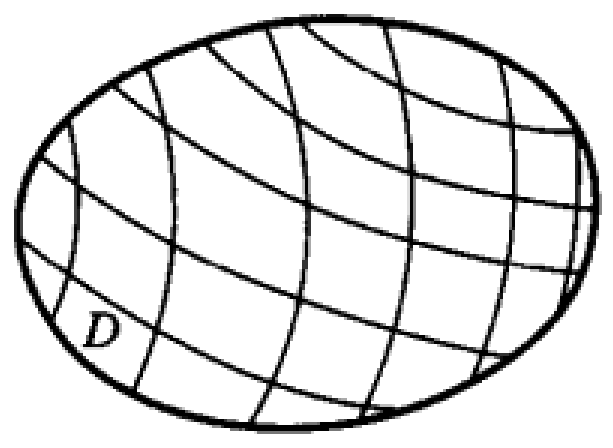
\includegraphics[width=0.32\textwidth]{work/figures/fig20-1}\caption{\relax}\label{fig:20-1}
\end{figure}

为了说清这个问题，我们先考虑平面上的多边形，平面上的多边形是指边界为有限条直线所围成的平面图形，它是有确定的面积的．对于一般的平面图形 $D$，我们自然想到用多边形去逼近它，这种逼近通常有两种，一种是外包的，一种是内含的．称多边形 $P_{1}$ 为 $D$ 的\emph{外包多边形}，如果对任意 $x\in D$，都有 $x\in P_{1}$；称多边形 $P_{2}$ 为 $D$ 的\emph{内含多边形}，如果对任意 $x\in P_{2}$，都有 $x\in D$（见图~\ref{fig:20-2}），这时 $P_{1}$，$P_{2}$ 都有面积，分别记为 $\left|P_{1}\right|$，$\left|P_{2}\right|$．显然，$D$ 要有面积，它必须是所有外包多边形面积的下确界
\[
\inf\left\{\,\left|P_{1}\right|\;\middle|\;P_{1}\ \text{为}\ D\ \text{的外包多边形}\,\right\},
\]
\begin{figure}[htbp]
\centering
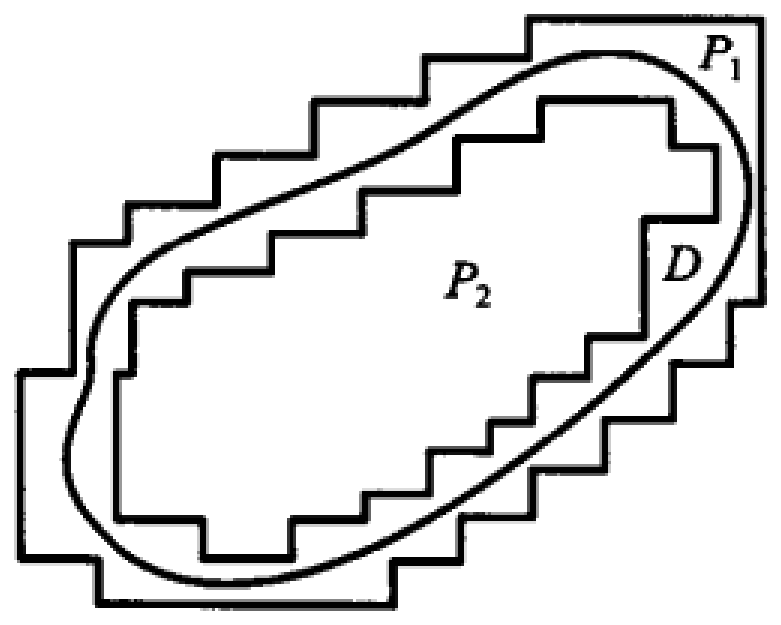
\includegraphics[width=0.34\textwidth]{work/figures/fig20-2}\caption{\relax}\label{fig:20-2}
\end{figure}
同时它也必须是所有内含多边形面积的上确界
\[
\sup\left\{\,\left|P_{2}\right|\;\middle|\;P_{2}\ \text{为}\ D\ \text{的内含多边形}\,\right\}.
\]
因此，$D$ 有面积当且仅当上述下确界等于上确界，即
\[
\inf\left\{\,\left|P_{1}\right|\;\middle|\;P_{1}\ \text{为}\ D\ \text{的外包多边形}\,\right\}
=\sup\left\{\,\left|P_{2}\right|\;\middle|\;P_{2}\ \text{为}\ D\ \text{的内含多边形}\,\right\},
\]
而且面积就等于这个上、下确界的公共值．

在定积分应用中，我们曾经介绍过如何求平面图形的面积．在这里需要指出的是，用定积分求出的面积同上述定义的面积是一致的．事实上，设 $f(x)\geqslant 0$ 在 $[a,b]$ 可积，则 $\displaystyle\int_{a}^{b}f(x)\,\mathrm{d}x$ 的几何意义是以 $f(x)$ 为顶的曲边梯形的面积．这时，$f(x)$ 的任一达布下和都是 $D$ 的一个内含多边形面积，$f(x)$ 的任一达布上和都是 $D$ 的一个外包多边形的面积．而达布下和的上确界则是 $f(x)$ 在 $[a,b]$ 的下积分 $\underline{I}$，达布上和的下确界是 $f(x)$ 在 $[a,b]$ 的上积分 $\overline{I}$．我们证明过，$f(x)$ 在 $[a,b]$ 可积，当且仅当上积分等于下积分：$\overline{I}=\underline{I}$，而且这公共值就等于 $f(x)$ 在 $[a,b]$ 的积分值．可见，这两个前后讲的面积概念实质上是一致的．

在定积分应用中，我们计算过用参数方程给出的曲线所包围的图形的面积．因此，我们知道，由逐段光滑曲线围成的平面图形是有面积的．

是否存在没有面积的平面图形呢？当然有，不可积函数的曲线构成的曲边梯形必然是没有面积的．例如，狄利克雷函数
\[
D(x)=\begin{cases}
1, & x\ \text{为有理数},\\
0, & x\ \text{为无理数},
\end{cases}
\]
则以它为顶的在 $[0,1]$ 上的曲边梯形
\[
D=\left\{(x,y)\mid 0\leqslant x\leqslant 1,0\leqslant y\leqslant D(x)\right\}
\]
就是没有面积的，因为它的外包多边形面积的下确界为 $1$，而内含多边形面积的上确界为 $0$．显然，$D$ 不是用逐段光滑曲线围成的平面图形．

在下面讨论二重积分时，总假定 $D$ 用逐段光滑曲线围成，因而是有面积的．

很容易把上述可求面积的概念推广到三维空间，建立可求体积的空间图形的概念．类似的讨论推广到一般的 $n$ 维空间也就没有任何困难了．

第二，什么叫 $D$ 的分法越来越细？对应于一维的 $\lambda=\max\limits_{1\leqslant i\leqslant n}\left\{\Delta x_{i}\right\}\to 0$，自然会认为可取 $\Delta\sigma_{i}$ 面积的最大者趋向于 $0$，但这实际上是不正确的．因为平面上一个图形 $\Delta\sigma_{i}$，无论它的面积多么小，都可能有其上的两点，它们的距离很大．这样，在求薄板质量的问题中，$f(\xi_{i},\eta_{i})\Delta\sigma_{i}$ 未必是 $\Delta\sigma_{i}$ 质量的近似值．为了保证 $\Delta\sigma_{i}$ 中任意两点的距离任意小，我们引入平面集合 $\bm{S}$ 的\emph{直径}的概念，称 $\bm{S}$ 中所有两点间的距离的上确界为 $\bm{S}$ 的直径，记为 $d(\bm{S})$，即
\[
d(\bm{S})=\sup\left\{r(P_{1},P_{2})\mid P_{1}\in\bm{S},P_{2}\in\bm{S}\right\},
\]
其中 $r(P_{1},P_{2})$ 表示 $P_{1}$ 与 $P_{2}$ 两点间的距离．有了集合直径的概念后，便可以令
\[
d=\max\left(d_{1},d_{2},\cdots,d_{n}\right),
\]
其中 $d_{i}=d(\Delta\sigma_{i})$ 是 $\Delta\sigma_{i}$ 的直径，则 $d\to 0$ 便描述了 $D$ 的分法越来越细，而这些显然都可以完全一样地推广到三维空间．

现在我们可以叙述二重积分的定义了．

\begin{definition}\label{def:20-1}
设 $D$ 是平面上可求面积的有界闭区域，$f(x,y)$ 定义在 $D$ 上，用任意曲线网将 $D$ 分成有限个可求面积的区域 $\Delta\sigma_{1},\Delta\sigma_{2},\cdots,\Delta\sigma_{n}$（称为 $D$ 的一个\emph{分法}），任取 $(\xi_{i},\eta_{i})\in\Delta\sigma_{i}$，$\Delta\sigma_{i}$ 既表示小块平面区域，也表示这小块区域的面积．作和
\[
\sigma=\sum_{i=1}^{n}f(\xi_{i},\eta_{i})\Delta\sigma_{i}.
\]
记 $d_{i}$ 为 $\Delta\sigma_{i}$ 的直径，$\lambda=\max\limits_{1\leqslant i\leqslant n}\left\{d_{i}\right\}$．如果当 $\lambda\to 0$ 时，$\sigma$ 的极限存在，则称 $f(x,y)$ 在 $D$ \emph{可积}，并称极限值为 $f(x,y)$ 在 $D$ 的\emph{二重积分}，记为
\[
\iint\limits_{D}f(P)\,\mathrm{d}\sigma\quad\text{或}\quad\iint\limits_{D}f(x,y)\,\mathrm{d}x\mathrm{d}y.
\]
也就是说，
\[
\iint_{D}f(x,y)\,\mathrm{d}x\mathrm{d}y=\iint_{D}f(P)\,\mathrm{d}\sigma=\lim_{\lambda\to 0}\sum_{i=1}^{n}f(\xi_{i},\eta_{i})\Delta\sigma_{i}.
\]
\end{definition}

和一元定积分的符号相类似，符号 $\displaystyle\iint_{D}f(P)\,\mathrm{d}\sigma$ 表示函数 $f(P)$ 与平面面积微元 $\mathrm{d}\sigma$ 乘积的``连续和''．而符号 $\displaystyle\iint_{D}f(x,y)\,\mathrm{d}x\mathrm{d}y$ 则侧重指出函数的积分变量是 $x$ 与 $y$，但也同时表示函数 $f(x,y)$ 与用平行于坐标轴的直线来作区域分法时的面积微元 $\mathrm{d}x\,\mathrm{d}y$ 的乘积之``连续和''（见图~\ref{fig:20-3}），以后将看到，与定积分不同的是，在变量代换时，他们不能看作 $x$，$y$ 微分的乘积．

\begin{figure}[htbp]
\centering
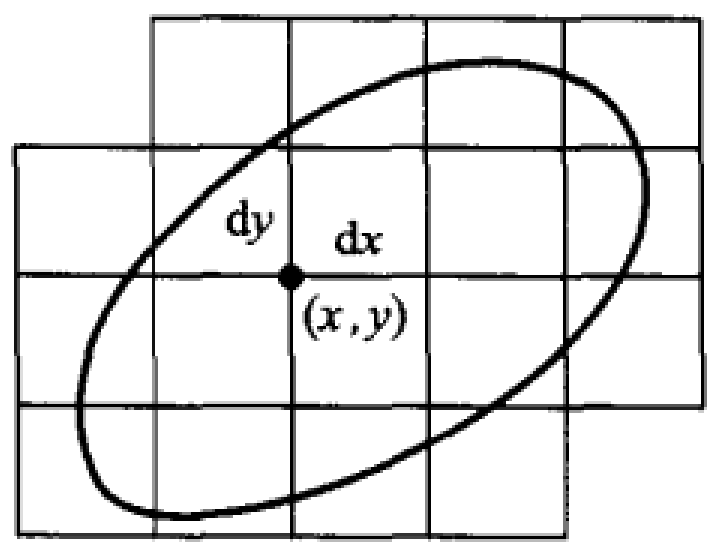
\includegraphics[width=0.32\textwidth]{work/figures/fig20-3}\caption{\relax}\label{fig:20-3}
\end{figure}

另外，值得说明的是，$\lambda$ 是依赖于 $D$ 的分法的．而和式 $\sigma$ 不仅依赖于 $D$ 的分法，而且还依赖于 $(\xi_{i},\eta_{i})\in\Delta\sigma_{i}$ 的取法．因此，所谓和式 $\sigma$ 的极限，严格地说应该用 $\varepsilon$-$\delta$ 语言来刻画．也就是说，若存在某定数 $I$，对任意给定的 $\varepsilon>0$，存在 $\delta>0$，使得对 $D$ 的任意分法 $T=\left\{\Delta\sigma_{i}\mid i=1,2,\cdots,n\right\}$，任意 $(\xi_{i},\eta_{i})\in\Delta\sigma_{i}$，只要 $\lambda=\max\limits_{1\leqslant i\leqslant n}\left\{d(\Delta\sigma_{i})\right\}<\delta$，就有
\[
\left|\sum_{i=1}^{n}f(\xi_{i},\eta_{i})\Delta\sigma_{i}-I\right|<\varepsilon,
\]
则称 $I$ 为函数 $f(x,y)$ 在 $D$ 的二重积分，记为
\[
I=\iint\limits_{D}f(x,y)\,\mathrm{d}x\mathrm{d}y.
\]

下面给出二重积分的几何解释．为简单起见，设 $D=[a,b]\times[c,d]$ 是一矩形区域，$f(x,y)\geqslant 0$ 在 $D$ 连续．这时，$z=f(x,y)$ 表示一曲面，而以 $D$ 为底，以曲面 $z=f(x,y)$ 为顶便构成一曲顶柱体．对于 $D$ 的任意分法（例如由平行于坐标轴的直线网给出）$\Delta\sigma_{i}$，$i=1,2,\cdots,n$，以及任取的 $(\xi_{i},\eta_{i})\in\Delta\sigma_{i}$，$f(\xi_{i},\eta_{i})\Delta\sigma_{i}$ 表示以 $\Delta\sigma_{i}$ 为底、以 $f(\xi_{i},\eta_{i})$ 为高的平顶柱体的体积，它是以 $\Delta\sigma_{i}$ 为底，以 $z=f(x,y)$ 为顶的曲顶柱体体积的近似，因此
\[
\sigma=\sum_{i=1}^{n}f(\xi_{i},\eta_{i})\Delta\sigma_{i}
\]
是整个 $D$ 上曲顶柱体体积的近似．当 $\lambda\to 0$ 时，这个和的极限便是 $D$ 上曲顶柱体的体积，而它也同时是 $f(x,y)$ 在 $D$ 的二重积分．故
\[
\iint_{D}f(x,y)\,\mathrm{d}x\mathrm{d}y=\lim_{\lambda\to 0}\sum_{i=1}^{n}f(\xi_{i},\eta_{i})\Delta\sigma_{i}
\]
的几何意义便是以 $D$ 为底，以 $z=f(x,y)$ 为顶的曲顶柱体的体积（图~\ref{fig:20-4}）．

\begin{figure}[htbp]
\centering
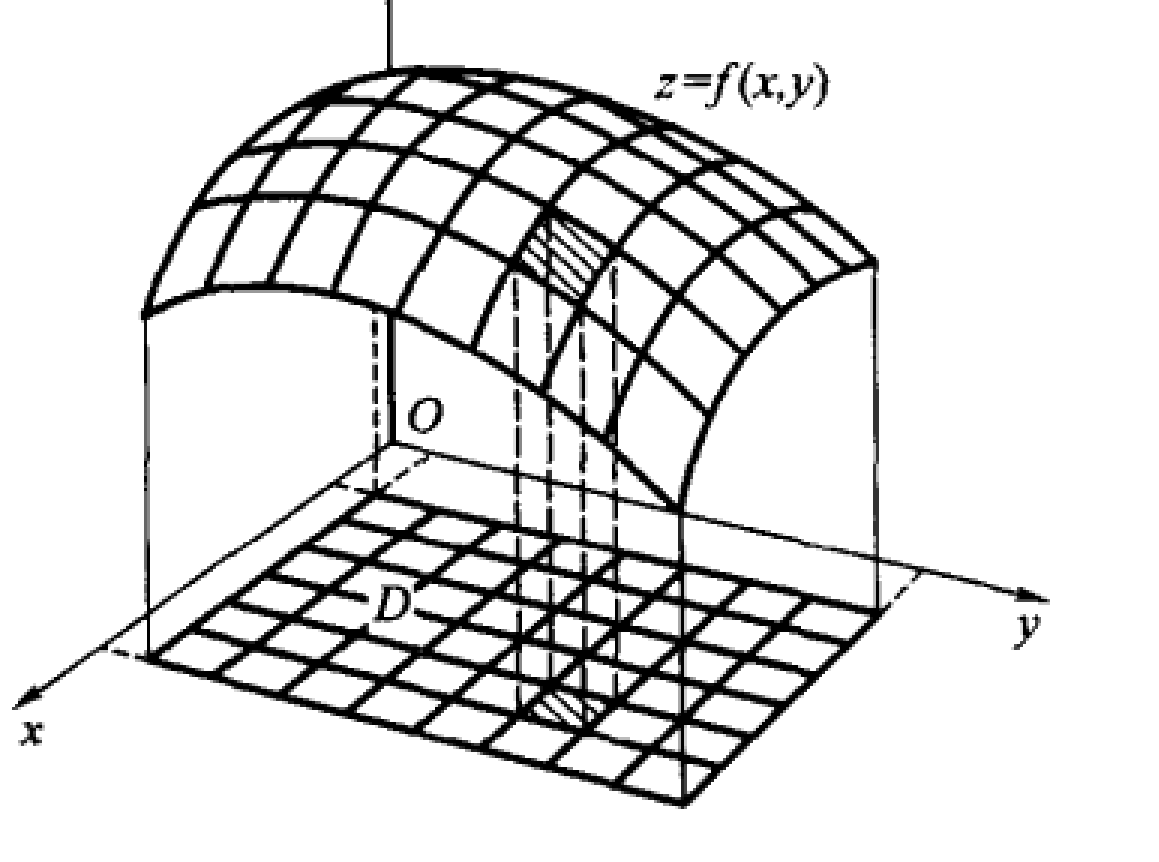
\includegraphics[width=0.42\textwidth]{work/figures/fig20-4}\caption{\relax}\label{fig:20-4}
\end{figure}

当 $D$ 不是矩形而是一般的区域时，$f(x,y)$ 在 $D$ 上的积分的几何解释仍然是以 $D$ 为底，以 $z=f(x,y)$ 为顶，由过 $D$ 的边界平行于 $z$ 轴的直线围成的曲顶柱体的体积，当然这时要假定 $f(x,y)\geqslant 0$（图~\ref{fig:20-5}）．

\begin{figure}[htbp]
\centering
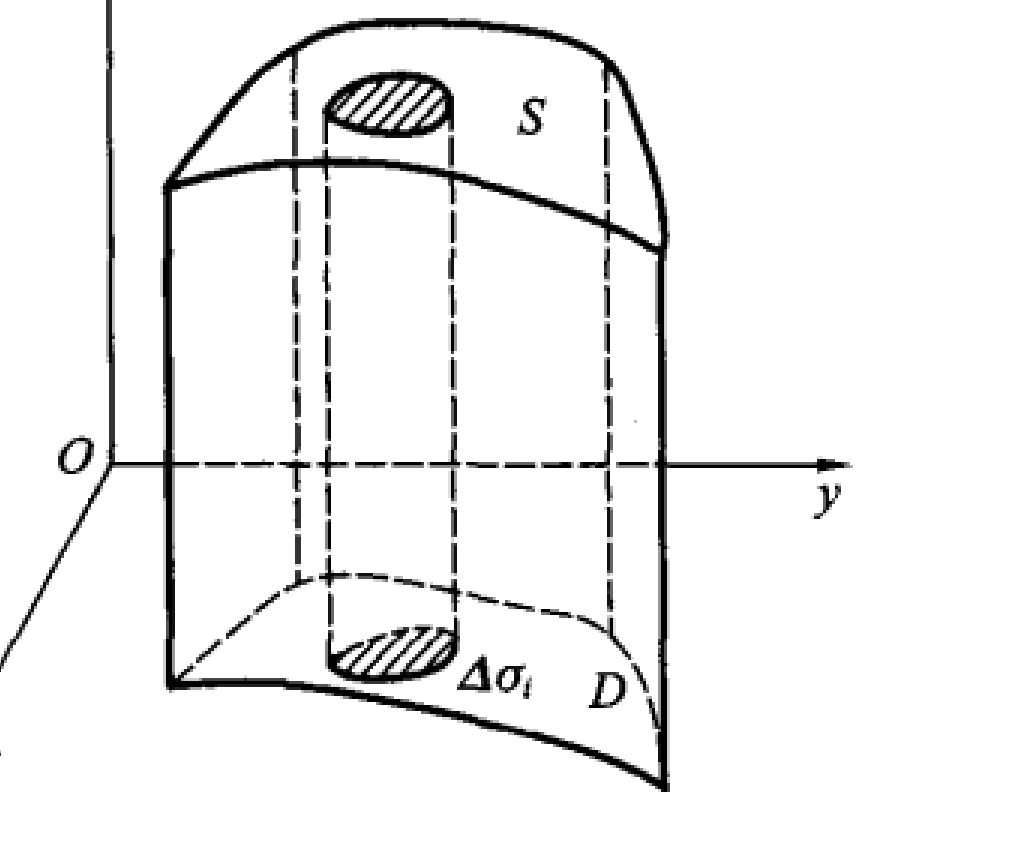
\includegraphics[width=0.40\textwidth]{work/figures/fig20-5}\caption{\relax}\label{fig:20-5}
\end{figure}

当 $f(x,y)$ 可正可负时，积分是相应的曲顶或曲底柱体的体积的代数和，这和一元函数定积分的情形是类似的．

可以完全仿照一元定积分建立二重积分的可积性理论．由此可以证明，逐段光滑曲线围成的有界闭区域 $D$ 上的连续函数在 $D$ 是可积的．还可进一步证明，若 $f$ 是有界闭区域 $D$ 上的有界函数，它只在 $D$ 内的有限段光滑曲线上间断，而在 $D$ 的其余地方均连续，则 $f$ 在 $D$ 可积．

不难由定义和可积性理论证明下面的二重积分基本性质．我们把证明留给读者作为习题．

\begin{ziti}
\item 若 $f(P)$ 在 $D$ 可积，$k$ 为常数，则 $kf(P)$ 也在 $D$ 可积，且
\[
\iint_{D}kf(P)\,\mathrm{d}\sigma=k\iint_{D}f(P)\,\mathrm{d}\sigma.
\]
\item 若 $f(P)$，$g(P)$ 都在 $D$ 可积，则 $f(P)\pm g(P)$，$f(P)g(P)$ 也在 $D$ 可积，并且
\[
\iint_{D}\left[f(P)\pm g(P)\right]\mathrm{d}\sigma=\iint_{D}f(P)\,\mathrm{d}\sigma\pm\iint_{D}g(P)\,\mathrm{d}\sigma.
\]
\item （可加性）若 $D$ 由 $D_{1}$，$D_{2}$ 组成：$D=D_{1}\cup D_{2}$，且 $D_{1}$，$D_{2}$ 除边界外不相交，则 $f(P)$ 在 $D$ 可积的充要条件是 $f(P)$ 在 $D_{1}$，$D_{2}$ 均可积，且
\[
\iint_{D}f(P)\,\mathrm{d}\sigma=\iint_{D_{1}}f(P)\,\mathrm{d}\sigma+\iint_{D_{2}}f(P)\,\mathrm{d}\sigma.
\]
\item （单调性）若 $f$ 与 $g$ 都在 $D$ 可积，且在 $D$ 的每点 $P$ 都有 $f(P)\leqslant g(P)$，则
\[
\iint_{D}f(P)\,\mathrm{d}\sigma\leqslant\iint_{D}g(P)\,\mathrm{d}\sigma.
\]
\item 若 $f(P)$ 在 $D$ 可积，则 $\left|f(P)\right|$ 也在 $D$ 可积，并且
\[
\left|\iint\limits_{D}f(P)\,\mathrm{d}\sigma\right|\leqslant\iint\limits_{D}\left|f(P)\right|\mathrm{d}\sigma.
\]
\item （积分中值定理）设 $D$ 是有界闭区域（因而是连通的），$f(P)$ 在 $D$ 上连续，则存在 $P_{0}\in D$，使得
\[
\iint_{D}f(P)\,\mathrm{d}\sigma=f(P_{0})\left|D\right|,
\]
其中 $\left|D\right|$ 表示 $D$ 的面积．
\end{ziti}

很容易把上述讨论推广到高维，建议读者写出三重积分
\[
\iiint\limits_{V}f(P)\,\mathrm{d}V\quad\text{或}\quad\iiint\limits_{V}f(x,y,z)\,\mathrm{d}x\mathrm{d}y\mathrm{d}z
\]
的定义，其中 $V$ 是三维空间中可求体积的有界闭区域．由于四维空间无法用图形画出来，故三重积分的几何解释——四维空间曲顶柱体的体积，就不如二重积分那么直观了．

\begin{xiti}
\item 证明性质（4），性质（6）．
\item 证明有界闭区域上的连续函数必可积．
\item 设 $\Omega$ 是可度量的平面图形或空间立体，$f$，$g$ 在 $\Omega$ 上连续，证明：
\begin{ziti}
\item 若在 $\Omega$ 上 $f(P)\geqslant 0$，且 $f(P)\not\equiv 0$，则 $\displaystyle\int_{\Omega}f(P)\,\mathrm{d}\Omega>0$；
\item 若在 $\Omega$ 的任何部分区域 $\Omega'\subset\Omega$ 上，有
\[
\int_{\Omega'}f(P)\,\mathrm{d}\Omega=\int_{\Omega'}g(P)\,\mathrm{d}\Omega,
\]
则在 $\Omega$ 上有 $f(P)\equiv g(P)$．
\end{ziti}
\item 设 $f(x)$ 在 $[a,b]$ 可积，$g(y)$ 在 $[c,d]$ 可积，则 $f(x)g(y)$ 在矩形区域 $D=[a,b]\times[c,d]$ 上可积，且
\[
\iint_{D}f(x)g(y)\,\mathrm{d}x\mathrm{d}y=\int_{a}^{b}f(x)\,\mathrm{d}x\int_{c}^{d}g(y)\,\mathrm{d}y.
\]
\item 若 $\left|f(x,y)\right|$ 在 $D$ 上可积，那么 $f(x,y)$ 在 $D$ 上是否可积？考察函数
\[
f(x,y)=\begin{cases}
1, & \text{若}\ x,y\ \text{都是有理数},\\
-1, & \text{若}\ x,y\ \text{至少有一个是无理数}
\end{cases}
\]
在 $[0,1]\times[0,1]$ 上的积分．
\item 设 $D=[0,1]\times[0,1]$，
\[
f(x,y)=\begin{cases}
1, & x\ \text{是有理数},\\
0, & x\ \text{是无理数},
\end{cases}
\]
证明 $f(x,y)$ 在 $D$ 上不可积．
\end{xiti}

\section{重积分化累次积分}\label{sec:20-2}

\subsection{二重积分化累次积分}

我们已经知道二重积分的几何解释是以 $z=f(x,y)$ 为顶，以 $D$ 为底的曲顶柱体的体积．先看 $D$ 为矩形 $[a,b]\times[c,d]$ 的情形．在含参变量积分的讨论中，我们已知 $\displaystyle\int_{c}^{d}f(x_{0},y)\,\mathrm{d}y$ 的几何意义是用垂直于 $x$ 轴的平面 $x=x_{0}$ 去截曲顶柱体，得一曲边梯形，曲顶为 $z=f(x_{0},y)$，$c\leqslant y\leqslant d$．该曲边梯形的面积便是
\[
A(x_{0})=\int_{c}^{d}f(x_{0},y)\,\mathrm{d}y.
\]
由 $x_{0}\in[a,b]$ 的任意性，知曲顶柱体的平行截面面积为 $A(x)$ $(a\leqslant x\leqslant b)$，因此它的体积是
\[
\iint_{D}f(x,y)\,\mathrm{d}x\mathrm{d}y=\int_{a}^{b}A(x)\,\mathrm{d}x=\int_{a}^{b}\mathrm{d}x\int_{c}^{d}f(x,y)\,\mathrm{d}y.
\]
类似地可以得到
\[
\iint_{D}f(x,y)\,\mathrm{d}x\mathrm{d}y=\int_{c}^{d}\mathrm{d}y\int_{a}^{b}f(x,y)\,\mathrm{d}x.
\]
一般地我们有下述定理．

\begin{theorem}\label{thm:20-1}
若 $f(x,y)$ 在矩形区域 $D=[a,b]\times[c,d]$ 上可积，并且对 $[a,b]$ 上的任何 $x$，含参变量积分
\[
A(x)=\int_{c}^{d}f(x,y)\,\mathrm{d}y
\]
存在，则
\[
\iint_{D}f(x,y)\,\mathrm{d}x\mathrm{d}y=\int_{a}^{b}\mathrm{d}x\int_{c}^{d}f(x,y)\,\mathrm{d}y.
\]
\end{theorem}

\begin{proof}
用平行于坐标轴的直线网
\[
a=x_{0}<x_{1}<\cdots<x_{n}=b,\qquad c=y_{0}<y_{1}<\cdots<y_{m}=d
\]
将 $D$ 分为若干个小矩形 $\Delta\sigma_{ij}=[x_{i-1},x_{i}]\times[y_{j-1},y_{j}]$．记 $f(x,y)$ 在 $\Delta\sigma_{ij}$ 的上、下确界分别为 $M_{ij}$ 和 $m_{ij}$．任取 $\xi_{i}\in[x_{i-1},x_{i}]$，则
\[
m_{ij}\Delta y_{j}\leqslant\int_{y_{j-1}}^{y_{j}}f(\xi_{i},y)\,\mathrm{d}y\leqslant M_{ij}\Delta y_{j},\quad i=1,2,\cdots,n,\ j=1,2,\cdots,m.
\]
对 $j$ 求和，得
\[
\sum_{j=1}^{m}m_{ij}\Delta y_{j}\leqslant\int_{c}^{d}f(\xi_{i},y)\,\mathrm{d}y=A(\xi_{i})\leqslant\sum_{j=1}^{m}M_{ij}\Delta y_{j},\quad i=1,2,\cdots,n.
\]
乘以 $\Delta x_{i}$ 后再对 $i$ 求和得
\[
\sum_{i=1}^{n}\sum_{j=1}^{m}m_{ij}\Delta x_{i}\Delta y_{j}\leqslant\sum_{i=1}^{n}A(\xi_{i})\Delta x_{i}\leqslant\sum_{i=1}^{n}\sum_{j=1}^{m}M_{ij}\Delta x_{i}\Delta y_{j}.
\]
当 $\lambda=\max\limits_{\begin{subarray}{c}1\leqslant i\leqslant n\\ 1\leqslant j\leqslant m\end{subarray}}\left\{\Delta\sigma_{ij}\ \text{的直径}\right\}\to 0$ 时，$\lambda'=\max\limits_{1\leqslant i\leqslant n}\left\{\Delta x_{i}\right\}\to 0$．由 $f(x,y)$ 在 $D$ 上可积知，上式左、右两端当 $\lambda\to 0$ 时有公共极限值 $\displaystyle\iint_{D}f(x,y)\,\mathrm{d}x\mathrm{d}y$，因此
\[
\lim_{\lambda'\to 0}\sum_{i=1}^{n}A(\xi_{i})\Delta x_{i}=\iint_{D}f(x,y)\,\mathrm{d}x\mathrm{d}y.
\]
由定积分定义即得
\[
\int_{a}^{b}A(x)\,\mathrm{d}x=\iint_{D}f(x,y)\,\mathrm{d}x\mathrm{d}y.
\]
把 $A(x)$ 的表达式代进去，便得
\[
\iint_{D}f(x,y)\,\mathrm{d}x\mathrm{d}y=\int_{a}^{b}\mathrm{d}x\int_{c}^{d}f(x,y)\,\mathrm{d}y.
\]
定理~\ref{thm:20-1}证完．
\end{proof}

当 $f(x,y)$ 取形式 $f_{1}(x)f_{2}(y)$ 时，定理~\ref{thm:20-1}的结论变成
\[
\iint_{D}f_{1}(x)f_{2}(y)\,\mathrm{d}x\mathrm{d}y=\int_{a}^{b}f_{1}(x)\,\mathrm{d}x\int_{c}^{d}f_{2}(y)\,\mathrm{d}y,
\]
这是§\ref{sec:20-1} 习题 4 曾经要读者证明的．

\begin{corollary}\label{cor:20-2-1}
设 $f(x,y)$ 在 $D=[a,b]\times[c,d]$ 上连续，则
\[
\iint_{D}f(x,y)\,\mathrm{d}x\mathrm{d}y=\int_{a}^{b}\mathrm{d}x\int_{c}^{d}f(x,y)\,\mathrm{d}y=\int_{c}^{d}\mathrm{d}y\int_{a}^{b}f(x,y)\,\mathrm{d}x.
\]
\end{corollary}

\begin{proof}
$f(x,y)$ 在 $D$ 上连续故可积，而且含参变量积分
\[
\int_{c}^{d}f(x,y)\,\mathrm{d}y\quad\text{和}\quad\int_{a}^{b}f(x,y)\,\mathrm{d}x
\]
都存在，由定理~\ref{thm:20-1}立得结论成立．
\end{proof}

定理~\ref{thm:20-1} 告诉我们在定理的条件下，二重积分可以化为累次积分来计算．而推论~\ref{cor:20-2-1} 告诉我们，当 $f$ 连续时，两个累次积分可以任意交换次序，或说累次积分与次序无关．

定理~\ref{thm:20-1}和推论~\ref{cor:20-2-1}揭示了重积分与累次积分的联系，二重积分的两个符号中，$\displaystyle\iint_{D}f(x,y)\,\mathrm{d}x\mathrm{d}y$ 较 $\displaystyle\iint_{D}f(P)\,\mathrm{d}\sigma$ 更好地反映出这一点．

\begin{example}\label{ex:20-2-1}
计算 $\displaystyle\iint_{D}x(x-y)^{2}\,\mathrm{d}x\mathrm{d}y$，其中 $D=[0,1]\times[0,1]$．
\end{example}

\begin{proof}[解]
\[
\begin{aligned}
\iint_{D}x(x-y)^{2}\,\mathrm{d}x\mathrm{d}y&=\int_{0}^{1}x\,\mathrm{d}x\int_{0}^{1}(x-y)^{2}\,\mathrm{d}y\\
&=\int_{0}^{1}-\frac{1}{3}x(x-y)^{3}\bigg|_{0}^{1}\,\mathrm{d}x=\frac{1}{3}\int_{0}^{1}x\left[x^{3}-(x-1)^{3}\right]\mathrm{d}x\\
&=\frac{1}{3}\int_{0}^{1}x(3x^{2}-3x+1)\,\mathrm{d}x=\frac{1}{3}\left[\frac{3}{4}x^{4}-x^{3}+\frac{1}{2}x^{2}\right]\bigg|_{0}^{1}\\
&=\frac{1}{12}.
\end{aligned}
\]
\end{proof}

下面要把定理~\ref{thm:20-1} 的矩形区域推广到一般的非矩形区域．我们先讨论简单区域．所谓\emph{简单区域} $D$ 是指区域的边界与平行于某一坐标轴（$x$ 轴或 $y$ 轴）的直线相交至多两点，或有部分边界是平行于坐标轴的．如图~\ref{fig:20-6} 和图~\ref{fig:20-7} 所示．对于简单区域 $D$，它至少可表为下列情形之一
\begin{equation}\label{eq:20-2-1}
D=\left\{(x,y)\mid y_{1}(x)\leqslant y\leqslant y_{2}(x),a\leqslant x\leqslant b\right\},
\tag{1}
\end{equation}
\begin{equation}\label{eq:20-2-2}
D=\left\{(x,y)\mid x_{1}(y)\leqslant x\leqslant x_{2}(y),c\leqslant y\leqslant d\right\}.
\tag{2}
\end{equation}

\begin{figure}[htbp]
\centering
\begin{tikzpicture}[scale=0.85,baseline=(current bounding box.center)]
  \fill[gray!12] (0.6,0.3) .. controls (1.2,1.6) and (2.6,1.9) .. (3.3,1.2)
    .. controls (3.6,0.5) and (2.6,0.1) .. (1.6,0.15) .. controls (1.0,0.18) .. (0.6,0.3);
  \draw[{-Latex}] (0,0) -- (4.2,0) node[below left] {$x$};
  \draw[{-Latex}] (0,0) -- (0,2.3) node[below left] {$y$};
  \draw (0.6,0.3) .. controls (1.2,1.6) and (2.6,1.9) .. (3.3,1.2);
  \draw (3.3,1.2) .. controls (3.6,0.5) and (2.6,0.1) .. (1.6,0.15) .. controls (1.0,0.18) .. (0.6,0.3);
  \draw[dashed] (1.9,0) -- (1.9,1.62);
  \node at (1.9,1.75) {$y_{2}(x)$};
  \node at (1.75,-0.28) {$y_{1}(x)$};
  \node at (0.55,-0.28) {$a$};
  \node at (3.35,-0.28) {$b$};
  \draw (1.9,0.18) -- (1.9,0.6);
\end{tikzpicture}\caption{\relax}\label{fig:20-6}
\end{figure}

\begin{figure}[htbp]
\centering
\begin{tikzpicture}[scale=0.85,baseline=(current bounding box.center)]
  \fill[gray!12] (0.6,0.3) .. controls (1.2,1.6) and (2.6,1.9) .. (3.3,1.2)
    .. controls (3.6,0.5) and (2.6,0.1) .. (1.6,0.15) .. controls (1.0,0.18) .. (0.6,0.3);
  \draw[{-Latex}] (0,0) -- (4.2,0) node[below left] {$x$};
  \draw[{-Latex}] (0,0) -- (0,2.3) node[below left] {$y$};
  \draw (0.6,0.3) .. controls (1.2,1.6) and (2.6,1.9) .. (3.3,1.2);
  \draw (3.3,1.2) .. controls (3.6,0.5) and (2.6,0.1) .. (1.6,0.15) .. controls (1.0,0.18) .. (0.6,0.3);
  \draw[dashed] (0,1.1) -- (3.45,1.1);
  \node[left] at (0,1.1) {\small $c$};
  \node[right] at (3.55,1.1) {\small $x_{2}(y)$};
  \node[left] at (0.45,1.1) {\small $x_{1}(y)$};
\end{tikzpicture}\caption{\relax}\label{fig:20-7}
\end{figure}

\begin{theorem}\label{thm:20-2}
设 $D$ 由\eqref{eq:20-2-1}式给出，$y_{1}(x)$，$y_{2}(x)$ 在 $[a,b]$ 上连续，$f(x,y)$ 在 $D$ 上连续，则
\[
\iint_{D}f(x,y)\,\mathrm{d}x\mathrm{d}y=\int_{a}^{b}\mathrm{d}x\int_{y_{1}(x)}^{y_{2}(x)}f(x,y)\,\mathrm{d}y.
\]
\end{theorem}

\begin{proof}
$y_{1}(x)$，$y_{2}(x)$ 在 $[a,b]$ 上连续，故 $y_{1}(x)$ 在 $[a,b]$ 上有最小值 $c$，$y_{2}(x)$ 在 $[a,b]$ 有最大值 $d$，故 $D\subset[a,b]\times[c,d]$．构造 $D$ 上的延拓函数 $\tilde{f}$
\[
\tilde{f}(x,y)=\begin{cases}
f(x,y), & (x,y)\in D,\\
0, & (x,y)\notin D.
\end{cases}
\]
由二重积分的性质（3）知 $\tilde{f}$ 在 $[a,b]\times[c,d]$ 可积，且
\[
\begin{aligned}
\iint\limits_{D}f(x,y)\,\mathrm{d}x\mathrm{d}y&=\iint\limits_{[a,b]\times[c,d]}\tilde{f}(x,y)\,\mathrm{d}x\mathrm{d}y
=\int_{a}^{b}\mathrm{d}x\int_{c}^{d}\tilde{f}(x,y)\,\mathrm{d}y\\
&=\int_{a}^{b}\mathrm{d}x\left[\int_{c}^{y_{1}(x)}\tilde{f}(x,y)\,\mathrm{d}y+\int_{y_{1}(x)}^{y_{2}(x)}\tilde{f}(x,y)\,\mathrm{d}y+\int_{y_{2}(x)}^{d}\tilde{f}(x,y)\,\mathrm{d}y\right]\\
&=\int_{a}^{b}\mathrm{d}x\int_{y_{1}(x)}^{y_{2}(x)}f(x,y)\,\mathrm{d}y.
\end{aligned}
\]
定理~\ref{thm:20-2}证完．
\end{proof}

同理，若 $D$ 由\eqref{eq:20-2-2}式给出，$x_{1}(y)$ 和 $x_{2}(y)$ 在 $[c,d]$ 上连续，$f(x,y)$ 在 $D$ 上连续，则
\[
\iint_{D}f(x,y)\,\mathrm{d}x\mathrm{d}y=\int_{c}^{d}\mathrm{d}y\int_{x_{1}(y)}^{x_{2}(y)}f(x,y)\,\mathrm{d}x.
\]
若 $D$ 既能用\eqref{eq:20-2-1}表示又能用\eqref{eq:20-2-2}表示，且 $x_{1}(y)$，$x_{2}(y)$，$y_{1}(x)$，$y_{2}(x)$ 均连续，$f$ 在 $D$ 上连续，则
\[
\iint_{D}f(x,y)\,\mathrm{d}x\mathrm{d}y=\int_{a}^{b}\mathrm{d}x\int_{y_{1}(x)}^{y_{2}(x)}f(x,y)\,\mathrm{d}y=\int_{c}^{d}\mathrm{d}y\int_{x_{1}(y)}^{x_{2}(y)}f(x,y)\,\mathrm{d}x.
\]

从上面二重积分化累次积分的公式可知，如果是先对 $y$ 积分，则 $y$ 的积分限一般是 $x$ 的函数，而最后积分的 $x$ 的积分限只能是常数；同理如果先对 $x$ 积分，则 $x$ 的积分限一般是 $y$ 的函数，而最后积分的 $y$ 的积分限只能是常数．

\begin{example}\label{ex:20-2-2}
求 $\displaystyle\iint_{D}\sqrt{4x^{2}-y^{2}}\,\mathrm{d}x\,\mathrm{d}y$，其中 $D$ 由 $y=0$，$x=1$，$y=x$ 围成．
\end{example}

\begin{proof}[解]
作出 $D$ 的图形．

\begin{figure}[htbp]
\centering
\begin{tikzpicture}[scale=1.15,baseline=(current bounding box.center)]
  \fill[gray!12] (0,0) -- (1,0) -- (1,1) -- cycle;
  \draw[{-Latex}] (-0.3,0) -- (1.6,0) node[below left] {$x$};
  \draw[{-Latex}] (0,-0.3) -- (0,1.6) node[below left] {$y$};
  \draw (0,0) -- (1,1) node[above right] {\small $y=x$};
  \draw (1,0) -- (1,1) node[above right] {\small $x=1$};
  \node at (0.65,0.22) {$D$};
  \node[below] at (1,0) {$1$};
\end{tikzpicture}\caption{\relax}\label{fig:20-8}
\end{figure}

用平行于 $y$ 轴的直线去截 $D$，则对每一 $x\in[0,1]$，有 $0\leqslant y\leqslant x$，故 $D$ 可表示为：$0\leqslant y\leqslant x$，$0\leqslant x\leqslant 1$．因此
\[
\iint_{D}\sqrt{4x^{2}-y^{2}}\,\mathrm{d}x\mathrm{d}y=\int_{0}^{1}\mathrm{d}x\int_{0}^{x}\sqrt{4x^{2}-y^{2}}\,\mathrm{d}y.
\]
对内层定积分作变量代换 $y=2x\sin t$，则
\[
\begin{aligned}
\iint\limits_{D}\sqrt{4x^{2}-y^{2}}\,\mathrm{d}x\mathrm{d}y&=\int_{0}^{1}\mathrm{d}x\int_{0}^{\frac{\pi}{6}}2x\cos t\cdot 2x\cos t\,\mathrm{d}t\\
&=4\int_{0}^{1}x^{2}\,\mathrm{d}x\int_{0}^{\frac{\pi}{6}}\cos^{2}t\,\mathrm{d}t\\
&=\frac{4}{3}x^{3}\bigg|_{0}^{1}\int_{0}^{\frac{\pi}{6}}\frac{1+\cos 2t}{2}\,\mathrm{d}t\\
&=\frac{4}{3}\left[\frac{1}{2}t+\frac{1}{4}\sin 2t\right]\bigg|_{0}^{\frac{\pi}{6}}=\frac{1}{3}\left[\frac{\pi}{3}+\frac{\sqrt{3}}{2}\right].
\end{aligned}
\]
\end{proof}

\begin{example}\label{ex:20-2-3}
求由 $z=xy$，$z=x+y$，$x+y=1$，$x=0$，$y=0$ 围成的区域的体积．
\end{example}

\begin{proof}[解]
空间区域如图~\ref{fig:20-9} 所示，它在 $Oxy$ 面上的投影 $D$ 由 $x+y=1$，$x=0$，$y=0$ 所围成（图~\ref{fig:20-10}）．用平行于 $y$ 轴的直线去截 $D$，则对每一 $x\in[0,1]$，有 $0\leqslant y\leqslant 1-x$．因此 $D$ 可表示为
\[
0\leqslant y\leqslant 1-x,\quad 0\leqslant x\leqslant 1.
\]

\begin{figure}[htbp]
\centering
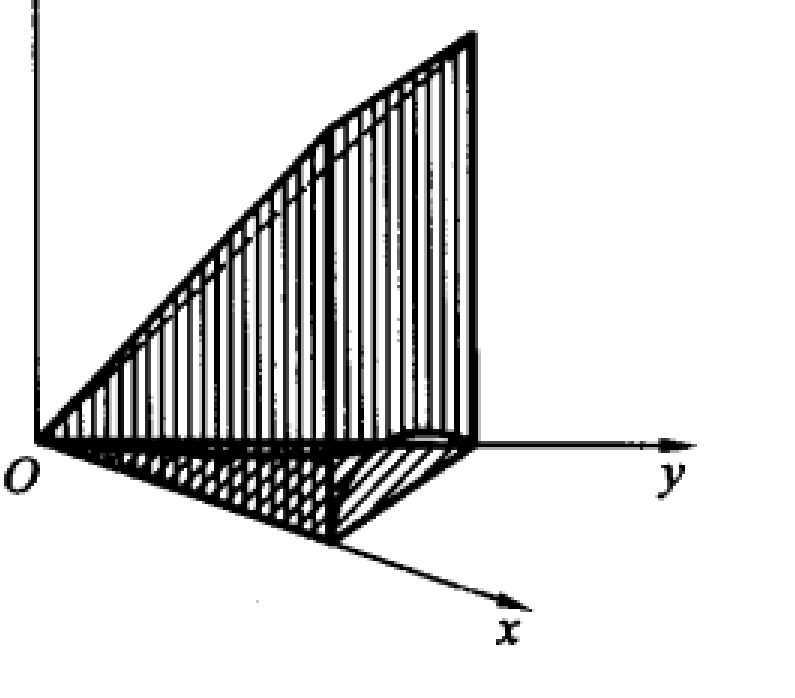
\includegraphics[width=0.34\textwidth]{work/figures/fig20-9}\caption{\relax}\label{fig:20-9}
\end{figure}

\begin{figure}[htbp]
\centering
\begin{tikzpicture}[scale=1.15,baseline=(current bounding box.center)]
  \fill[gray!12] (0,0) -- (1.3,0) -- (0,1.3) -- cycle;
  \draw[{-Latex}] (-0.3,0) -- (1.8,0) node[below left] {$x$};
  \draw[{-Latex}] (0,-0.3) -- (0,1.8) node[below left] {$y$};
  \draw (1.3,0) -- (0,1.3) node[above left] {\small $x+y=1$};
  \node at (0.4,0.35) {$D$};
  \node[below] at (1.3,0) {$1$};
  \node[left] at (0,1.3) {$1$};
\end{tikzpicture}\caption{\relax}\label{fig:20-10}
\end{figure}

故体积 $V$ 为
\[
\begin{aligned}
V&=\iint\limits_{D}\left[(x+y)-xy\right]\mathrm{d}x\mathrm{d}y\\
&=\int_{0}^{1}\mathrm{d}x\int_{0}^{1-x}(x+y-xy)\,\mathrm{d}y\\
&=\int_{0}^{1}\left[xy+\frac{(1-x)}{2}y^{2}\right]\bigg|_{0}^{1-x}\,\mathrm{d}x\\
&=\int_{0}^{1}\left[x(1-x)+\frac{1}{2}(1-x)^{3}\right]\mathrm{d}x\\
&=\left[\frac{1}{2}x^{2}-\frac{1}{3}x^{3}-\frac{1}{8}(1-x)^{4}\right]\bigg|_{0}^{1}=\frac{7}{24}.
\end{aligned}
\]
\end{proof}

\begin{example}\label{ex:20-2-4}
用两种不同的顺序将二重积分
\[
I=\iint\limits_{D}f(x,y)\,\mathrm{d}x\mathrm{d}y
\]
化为累次积分，其中 $D$ 由 $y=0$，$y=x^{3}$，$x+y=2$ 围成．
\end{example}

\begin{proof}[解]
作图．

两曲线 $y=x^{3}$ 和 $x+y=2$ 的交点为 $(1,1)$．

考虑先对 $y$ 积分．用平行于 $y$ 轴的直线去截 $D$，当 $x\in[0,1]$ 时有 $0\leqslant y\leqslant x^{3}$；当 $x\in[1,2]$ 时有 $0\leqslant y\leqslant 2-x$．这样 $D$ 可分为两部分 $D_{1}$ 和 $D_{2}$，其中
\[
\begin{aligned}
&D_{1}:\ 0\leqslant y\leqslant x^{3},\ 0\leqslant x\leqslant 1,\\
&D_{2}:\ 0\leqslant y\leqslant 2-x,\ 1\leqslant x\leqslant 2.
\end{aligned}
\]

\begin{figure}[htbp]
\centering
\begin{tikzpicture}[scale=1.0,baseline=(current bounding box.center)]
  \fill[gray!12] (0,0) plot[smooth,domain=0:1] (\x,\x*\x*\x) -- (2,0) -- cycle;
  \draw[{-Latex}] (-0.3,0) -- (2.5,0) node[below left] {$x$};
  \draw[{-Latex}] (0,-0.3) -- (0,2.5) node[below left] {$y$};
  \draw[smooth,domain=0:1.15] plot (\x,{\x*\x*\x}) node[right] {\small $y=x^{3}$};
  \draw (1,1) -- (2,0) node[below right] {\small $x+y=2$};
  \node at (0.85,0.35) {$D$};
  \node[below] at (1,0) {$1$};
  \node[below] at (2,0) {$2$};
  \node[left] at (0,1) {$1$};
  \draw[dashed] (1,0) -- (1,1);
\end{tikzpicture}\caption{\relax}\label{fig:20-11}
\end{figure}

因此
\[
\begin{aligned}
\iint_{D}f(x,y)\,\mathrm{d}x\mathrm{d}y&=\int_{0}^{1}\mathrm{d}x\int_{0}^{x^{3}}f(x,y)\,\mathrm{d}y+\\
&\quad \int_{1}^{2}\mathrm{d}x\int_{0}^{2-x}f(x,y)\,\mathrm{d}y.
\end{aligned}
\]
再考虑先对 $x$ 积分．用平行于 $x$ 轴的直线去截 $D$，则对每一 $y\in[0,1]$，有 $y^{\frac{1}{3}}\leqslant x\leqslant 2-y$，故 $D$ 又可表为
\[
D:\ y^{\frac{1}{3}}\leqslant x\leqslant 2-y,\ 0\leqslant y\leqslant 1.
\]
因此
\[
\iint_{D}f(x,y)\,\mathrm{d}x\mathrm{d}y=\int_{0}^{1}\mathrm{d}y\int_{y^{\frac{1}{3}}}^{2-y}f(x,y)\,\mathrm{d}x.
\]
\end{proof}

\begin{example}\label{ex:20-2-5}
计算积分
\[
I=\int_{0}^{1}\mathrm{d}x\int_{x}^{\sqrt{x}}\frac{\sin y}{y}\,\mathrm{d}y.
\]
\end{example}

\begin{proof}[解]
这个累次积分是先对 $y$ 积分，再对 $x$ 积分．而 $\dfrac{\sin y}{y}$ 的原函数不能用初等函数表示．因此按上述顺序进行累次积分是行不通的．为此考虑改变积分的顺序．

根据积分限知，将上述积分表为二重积分时，积分区域 $D$ 为 $x\leqslant y\leqslant\sqrt{x}$，$0\leqslant x\leqslant 1$．即 $D$ 由曲线 $y=x$，$y=\sqrt{x}$，$x=0$ 和 $x=1$ 围成．作出 $D$ 的图形如图~\ref{fig:20-12}．用平行于 $x$ 轴的直线去截 $D$，对每一 $y\in[0,1]$，有 $y^{2}\leqslant x\leqslant y$，于是有
\[
\begin{aligned}
I&=\int_{0}^{1}\mathrm{d}x\int_{x}^{\sqrt{x}}\frac{\sin y}{y}\,\mathrm{d}y=\int_{0}^{1}\mathrm{d}y\int_{y^{2}}^{y}\frac{\sin y}{y}\,\mathrm{d}x\\
&=\int_{0}^{1}\frac{\sin y}{y}(y-y^{2})\,\mathrm{d}y=\int_{0}^{1}\sin y\,\mathrm{d}y-\int_{0}^{1}y\sin y\,\mathrm{d}y\\
&=-\cos y\left|_{0}^{1}-(-\cos y+\sin y)\right|_{0}^{1}=1-\sin 1.
\end{aligned}
\]

\begin{figure}[htbp]
\centering
\begin{tikzpicture}[scale=1.3,baseline=(current bounding box.center)]
  \fill[gray!12] (0,0) plot[smooth,domain=0:1] (\x,{sqrt(\x)}) -- (1,1) plot[smooth,domain=1:0] (\x,\x) -- cycle;
  \draw[{-Latex}] (-0.2,0) -- (1.5,0) node[below left] {$x$};
  \draw[{-Latex}] (0,-0.2) -- (0,1.5) node[below left] {$y$};
  \draw[smooth,domain=0:1] plot (\x,{sqrt(\x)}) node[above right] {\small $y=\sqrt{x}$};
  \draw (0,0) -- (1,1) node[below right] {\small $y=x$};
  \node at (0.55,0.6) {$D$};
  \node[below] at (1,0) {$1$};
  \node[left] at (0,1) {$1$};
  \draw[dashed] (1,1) -- (1,0);
  \draw[dashed] (1,1) -- (0,1);
\end{tikzpicture}\caption{\relax}\label{fig:20-12}
\end{figure}

从此例可见，将二重积分化为累次积分时，积分次序对计算是有影响的，选择得不好，可能使计算很繁，甚至积不出来．顺便指出，对上述累次积分除了用改变积分次序的方法进行计算外，还可用分部积分方法进行计算．记
\[
A(x)=\int_{x}^{\sqrt{x}}\frac{\sin y}{y}\,\mathrm{d}y,
\]
则由分部积分得
\[
\begin{aligned}
I&=\int_{0}^{1}A(x)\,\mathrm{d}x=xA(x)\bigg|_{0}^{1}-\int_{0}^{1}xA'(x)\,\mathrm{d}x\\
&=A(1)-\int_{0}^{1}x\left(\frac{\sin\sqrt{x}}{\sqrt{x}}\frac{1}{2\sqrt{x}}-\frac{\sin x}{x}\right)\mathrm{d}x\\
&=-\int_{0}^{1}\frac{1}{2}\sin\sqrt{x}\,\mathrm{d}x+\int_{0}^{1}\sin x\,\mathrm{d}x,
\end{aligned}
\]
在第一项中令 $\sqrt{x}=t$，得
\[
I=-\int_{0}^{1}t\sin t\,\mathrm{d}t+\int_{0}^{1}\sin x\,\mathrm{d}x=1-\sin 1.
\]
\end{proof}

将二重积分化为累次积分，其中最基本的步骤就是根据二重积分的积分域 $D$ 确定累次积分的积分限．这是初学者感到不易掌握和容易出错的地方．作出 $D$ 的图形可以给我们提供非常直观的认识，减少出错率，因此切不可忽视作图．定积分限的方法必须很好地掌握，它是计算重积分最基础的内容．

如果区域 $D$ 能分解成有限个没有公共内点的简单区域的并，则对每个简单区域应用上述积分公式，我们便能计算很多较复杂区域的二重积分．

\subsection{三重积分化累次积分}

对于三重积分
\[
\iiint_{V}f(x,y,z)\,\mathrm{d}x\mathrm{d}y\mathrm{d}z,
\]
其计算也是化为累次积分来计算．下面我们不加证明地给出化累次积分的公式，其中出现的积分都假定是存在的．

（1）$V$ 是长方体 $[a,b]\times[c,d]\times[e,f]$，则有公式
\[
\iiint_{V}f(x,y,z)\,\mathrm{d}x\mathrm{d}y\mathrm{d}z=\int_{a}^{b}\mathrm{d}x\int_{c}^{d}\mathrm{d}y\int_{e}^{f}f(x,y,z)\,\mathrm{d}z.
\]
它完全可以类似于定理~\ref{thm:20-1}一样加以证明．把后面两个累次积分写成重积分，便得
\[
\iiint_{V}f(x,y,z)\,\mathrm{d}x\mathrm{d}y\mathrm{d}z=\int_{a}^{b}\mathrm{d}x\iint_{[c,d]\times[e,f]}f(x,y,z)\,\mathrm{d}y\mathrm{d}z,
\]
这可以看作，对每个固定的 $x$，先对截面积分，然后对 $x$ 按 $a$ 到 $b$ 积分，便得在整个立体 $V$ 的积分．

公式也可以写成
\[
\iiint_{V}f(x,y,z)\,\mathrm{d}x\mathrm{d}y\mathrm{d}z=\iint_{[a,b]\times[c,d]}\mathrm{d}x\mathrm{d}y\int_{e}^{f}f(x,y,z)\,\mathrm{d}z,
\]
这可以看作，在 $[a,b]\times[c,d]$ 中固定的一点 $(x,y)$，先对 $z$ 从 $e$ 到 $f$ 积分，然后再对 $(x,y)$ 在整个 $[a,b]\times[c,d]$ 积分，便得在整个立体 $V$ 的积分．

\begin{figure}[htbp]
\centering
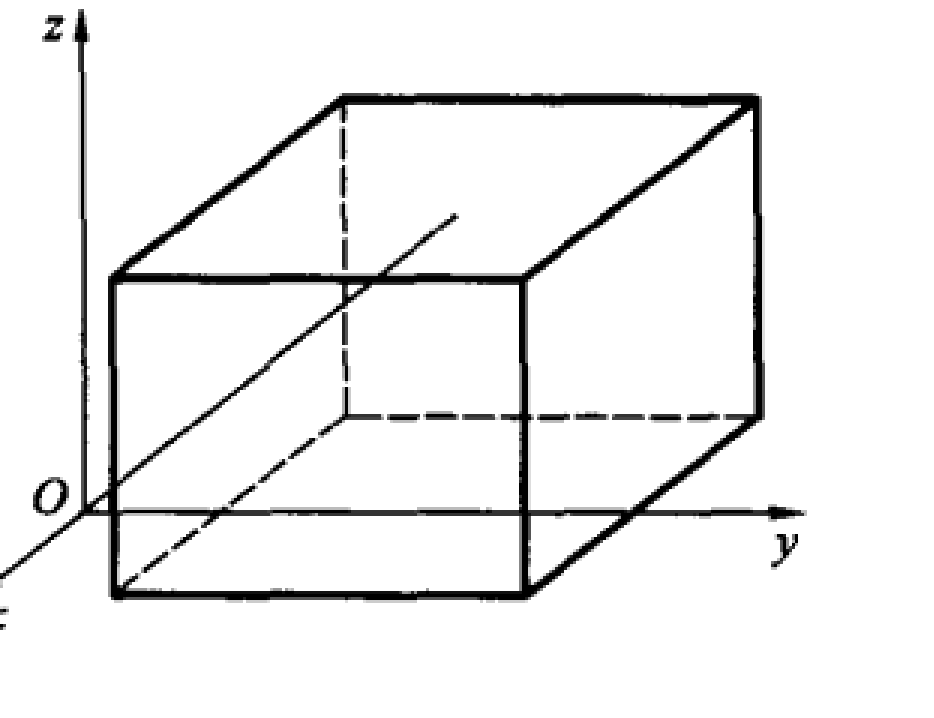
\includegraphics[width=0.32\textwidth]{work/figures/fig20-13}\caption{\relax}\label{fig:20-13}
\end{figure}

（2）设空间立体界于平面 $z=e$ 和 $z=f$ 之间，对每一 $z\in[e,f]$，用平行于 $Oxy$ 面的平面 $z=z$ 去截立体 $V$ 得一平面图形 $D_{z}$（见图~\ref{fig:20-14}），则有
\[
\iiint_{V}f(x,y,z)\,\mathrm{d}x\mathrm{d}y\mathrm{d}z=\int_{e}^{f}\mathrm{d}z\iint_{D_{z}}f(x,y,z)\,\mathrm{d}x\mathrm{d}y.
\]
其中 $\displaystyle\iint_{D_{z}}f(x,y,z)\,\mathrm{d}x\,\mathrm{d}y$ 是展布在平面图形 $D_{z}$ 上的二重积分，$z$ 相对固定不变．一般来说当 $z$ 在 $[e,f]$ 上变动时，所得到的平面图形 $D_{z}$ 是不同的，即 $D_{z}$ 是依赖于 $z$ 的．若 $D_{z}$ 可表示为 $x_{1}(y,z)\leqslant x\leqslant x_{2}(y,z)$，$y_{1}(z)\leqslant y\leqslant y_{2}(z)$（见图~\ref{fig:20-15}），则
\[
\begin{aligned}
\iiint_{V}f(x,y,z)\,\mathrm{d}x\mathrm{d}y\mathrm{d}z&=\int_{e}^{f}\mathrm{d}z\iint_{D_{z}}f(x,y,z)\,\mathrm{d}x\mathrm{d}y\\
&=\int_{e}^{f}\mathrm{d}z\int_{y_{1}(z)}^{y_{2}(z)}\mathrm{d}y\int_{x_{1}(y,z)}^{x_{2}(y,z)}f(x,y,z)\,\mathrm{d}x.
\end{aligned}
\]

\begin{figure}[htbp]
\centering
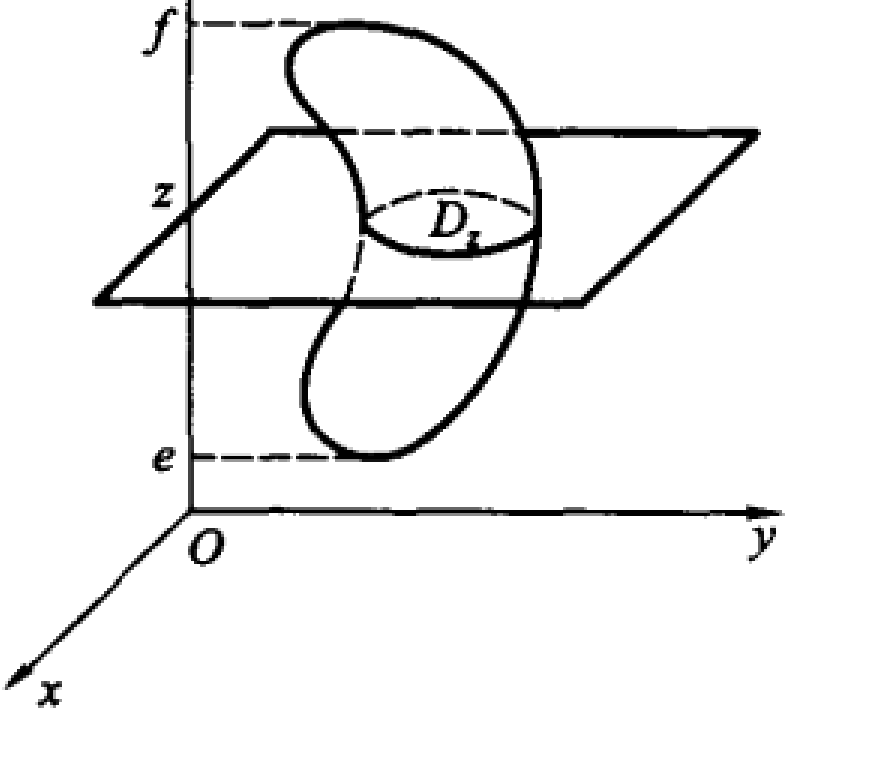
\includegraphics[width=0.32\textwidth]{work/figures/fig20-14}\caption{\relax}\label{fig:20-14}
\end{figure}

\begin{figure}[htbp]
\centering
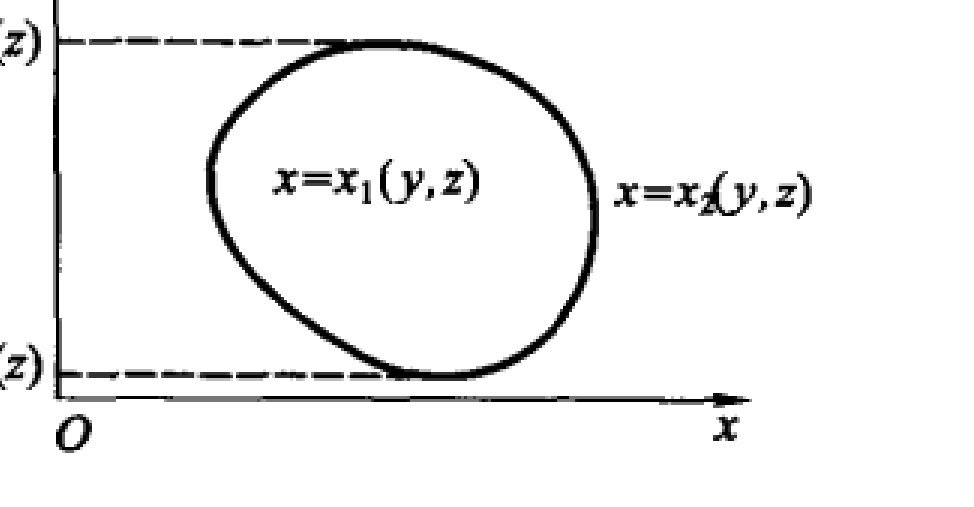
\includegraphics[width=0.34\textwidth]{work/figures/fig20-15}\caption{\relax}\label{fig:20-15}
\end{figure}

通常，先积分者，其积分限是后积分变量的函数，而最后积分者，其积分限只能是常数．

（3）设空间立体 $V$ 在 $Oxy$ 面上的投影 $D$ 是平面上的简单区域．平行于 $z$ 轴且通过 $D$ 的内点的直线与 $V$ 的边界相交至多两点（图~\ref{fig:20-16}）．记下面一点所在的边界曲面为 $z_{1}(x,y)$，上面一点所在的边界曲面为 $z_{2}(x,y)$，则有公式
\[
\iiint_{V}f(x,y,z)\,\mathrm{d}x\mathrm{d}y\mathrm{d}z=\iint_{D}\mathrm{d}x\mathrm{d}y\int_{z_{1}(x,y)}^{z_{2}(x,y)}f(x,y,z)\,\mathrm{d}z.
\]

\begin{figure}[htbp]
\centering
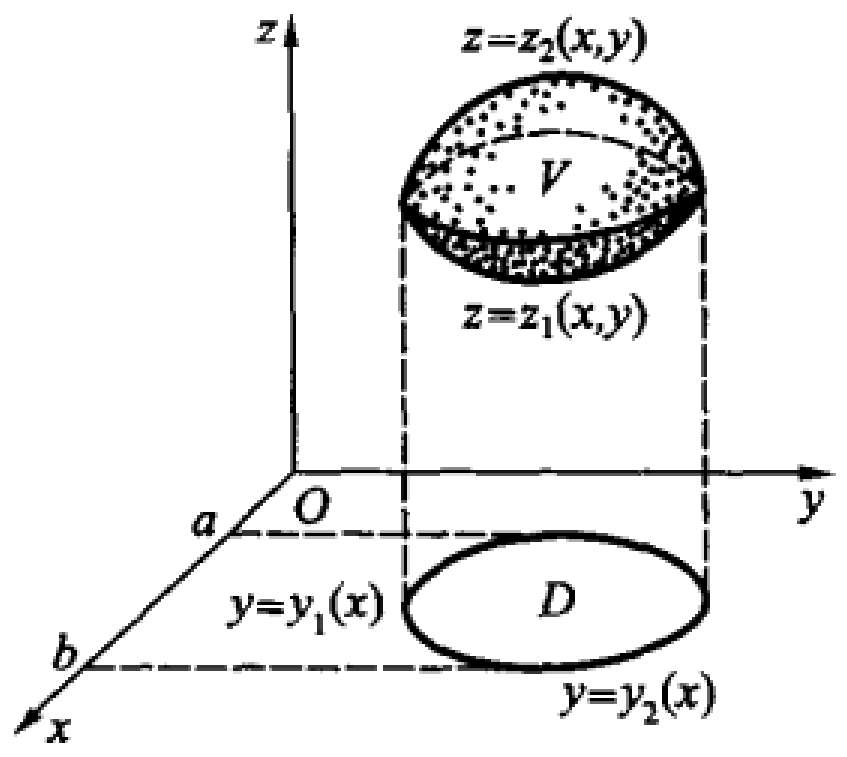
\includegraphics[width=0.32\textwidth]{work/figures/fig20-16}\caption{\relax}\label{fig:20-16}
\end{figure}

又若 $D$ 可表为 $y_{1}(x)\leqslant y\leqslant y_{2}(x)$，$a\leqslant x\leqslant b$，则有
\[
\iiint_{V}f(x,y,z)\,\mathrm{d}x\mathrm{d}y\mathrm{d}z=\int_{a}^{b}\mathrm{d}x\int_{y_{1}(x)}^{y_{2}(x)}\mathrm{d}y\int_{z_{1}(x,y)}^{z_{2}(x,y)}f(x,y,z)\,\mathrm{d}z.
\]

\begin{example}\label{ex:20-2-6}
计算
\[
I=\iiint_{V}\frac{\mathrm{d}x\mathrm{d}y\mathrm{d}z}{(1+x+y+z)^{3}},
\]
其中 $V$ 由 $x=0$，$y=0$，$z=0$，$x+y+z=1$ 围成．
\end{example}

\begin{proof}[解]
区域 $V$ 如图~\ref{fig:20-17}，$V$ 在 $Oxy$ 平面的投影由 $x=0$，$y=0$，$x+y=1$ 围成，这时区域 $V$ 的底为 $z=0$，顶为 $z=1-x-y$．因此
\[
\begin{aligned}
I&=\iint_{D}\mathrm{d}x\mathrm{d}y\int_{0}^{1-x-y}\frac{\mathrm{d}z}{(1+x+y+z)^{3}}\\
&=\int_{0}^{1}\mathrm{d}x\int_{0}^{1-x}\mathrm{d}y\int_{0}^{1-x-y}\frac{\mathrm{d}z}{(1+x+y+z)^{3}}\\
&=\int_{0}^{1}\mathrm{d}x\int_{0}^{1-x}\frac{-1}{2(1+x+y+z)^{2}}\bigg|_{0}^{1-x-y}\,\mathrm{d}y\\
&=\int_{0}^{1}\mathrm{d}x\int_{0}^{1-x}\frac{1}{2}\left[\frac{1}{(1+x+y)^{2}}-\frac{1}{4}\right]\mathrm{d}y\\
&=\frac{1}{2}\int_{0}^{1}\left[-\frac{1}{(1+x+y)}-\frac{y}{4}\right]\bigg|_{0}^{1-x}\,\mathrm{d}x\\
&=\frac{1}{2}\int_{0}^{1}\left(\frac{1}{x+1}-\frac{3-x}{4}\right)\mathrm{d}x\\
&=\frac{1}{2}\left[\ln(1+x)\big|_{0}^{1}+\frac{(3-x)^{2}}{8}\bigg|_{0}^{1}\right]=\frac{1}{2}\left(\ln 2-\frac{5}{8}\right).
\end{aligned}
\]
\end{proof}

\begin{figure}[htbp]
\centering
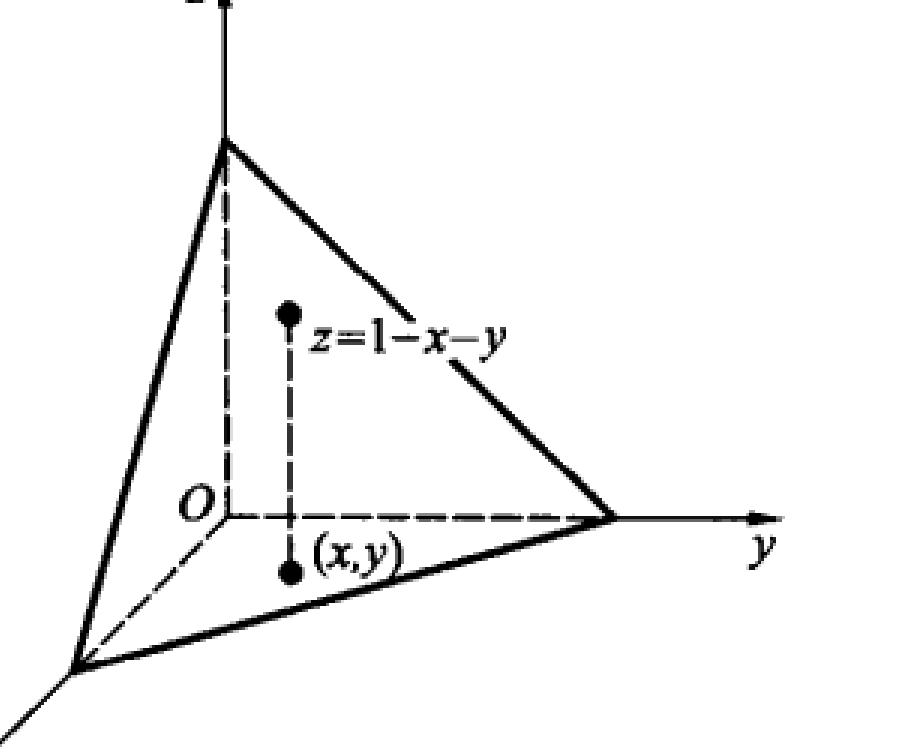
\includegraphics[width=0.32\textwidth]{work/figures/fig20-17}\caption{\relax}\label{fig:20-17}
\end{figure}

\begin{example}\label{ex:20-2-7}
求 $\displaystyle I=\iiint_{V}(x^{2}+y^{2}+z^{2})\,\mathrm{d}x\,\mathrm{d}y\,\mathrm{d}z$，其中 $V$ 是椭球体
\[
\frac{x^{2}}{a^{2}}+\frac{y^{2}}{b^{2}}+\frac{z^{2}}{c^{2}}\leqslant 1.
\]
\end{example}

\begin{proof}[解]
作图．

\begin{figure}[htbp]
\centering
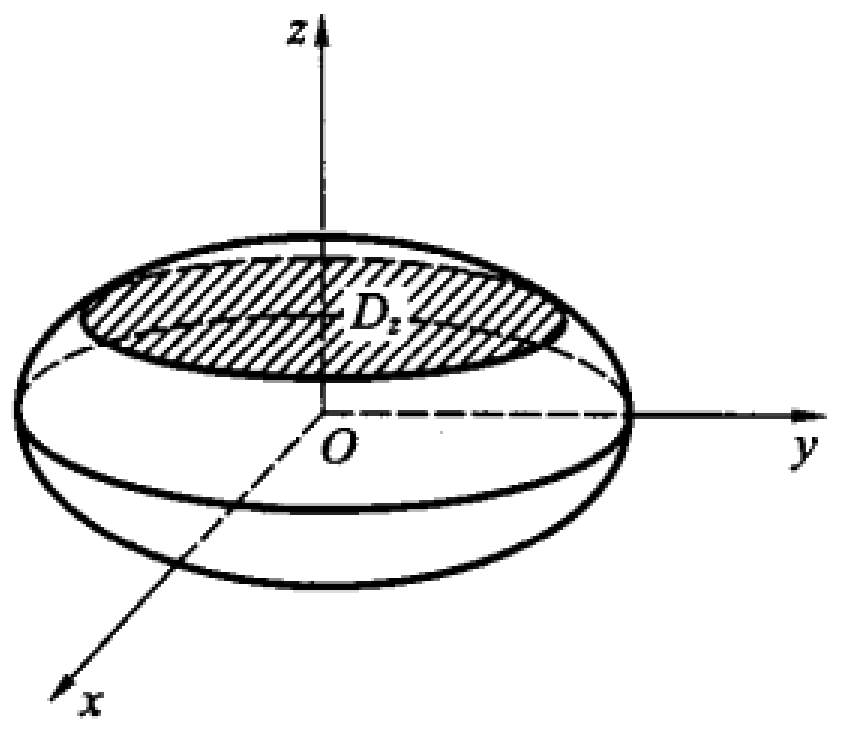
\includegraphics[width=0.32\textwidth]{work/figures/fig20-18}\caption{\relax}\label{fig:20-18}
\end{figure}

显然，对于每一 $z\in[-c,c]$，用平行于 $Oxy$ 面的平面 $z=z$ 去截椭球体，得一椭圆面 $D_{z}$：
\[
\frac{x^{2}}{a^{2}\left(1-\dfrac{z^{2}}{c^{2}}\right)}+\frac{y^{2}}{b^{2}\left(1-\dfrac{z^{2}}{c^{2}}\right)}\leqslant 1,
\]
它的面积为
\[
\pi\sqrt{a^{2}\left(1-\frac{z^{2}}{c^{2}}\right)}\cdot\sqrt{b^{2}\left(1-\frac{z^{2}}{c^{2}}\right)}=\pi ab\left(1-\frac{z^{2}}{c^{2}}\right).
\]
显然
\[
I=\iiint\limits_{V}x^{2}\,\mathrm{d}x\mathrm{d}y\mathrm{d}z+\iiint\limits_{V}y^{2}\,\mathrm{d}x\mathrm{d}y\mathrm{d}z+\iiint\limits_{V}z^{2}\,\mathrm{d}x\mathrm{d}y\mathrm{d}z.
\]
由前面的公式有
\[
\iiint_{V}z^{2}\,\mathrm{d}x\mathrm{d}y\mathrm{d}z=\int_{-c}^{c}z^{2}\,\mathrm{d}z\iint_{D_{z}}\mathrm{d}x\mathrm{d}y.
\]
根据二重积分的几何意义知，$\displaystyle\iint_{D_{z}}\mathrm{d}x\,\mathrm{d}y=D_{z}$ 的面积．因此
\[
\begin{aligned}
\iiint_{V}z^{2}\,\mathrm{d}x\mathrm{d}y\mathrm{d}z&=\int_{-c}^{c}z^{2}\pi ab\left(1-\frac{z^{2}}{c^{2}}\right)\mathrm{d}z\\
&=2\pi ab\int_{0}^{c}\left(z^{2}-\frac{1}{c^{2}}z^{4}\right)\mathrm{d}z=\frac{4}{15}\pi abc^{3}.
\end{aligned}
\]
由椭球体的对称性易见
\[
\iiint_{V}x^{2}\,\mathrm{d}x\mathrm{d}y\mathrm{d}z=\frac{4}{15}\pi a^{3}bc;\qquad
\iiint_{V}y^{2}\,\mathrm{d}x\mathrm{d}y\mathrm{d}z=\frac{4}{15}\pi ab^{3}c.
\]
于是
\[
I=\iiint\limits_{V}(x^{2}+y^{2}+z^{2})\,\mathrm{d}x\mathrm{d}y\mathrm{d}z=\frac{4}{15}\pi abc(a^{2}+b^{2}+c^{2}).
\]
\end{proof}

在上例的求解过程中，我们用到了以下一些技巧，使计算大大简化了．

（1）利用积分域的对称性和被积函数的对称性，只需计算三项积分中的一项．

（2）我们选择了最后对 $z$ 积分，即
\[
\iiint_{V}z^{2}\,\mathrm{d}x\mathrm{d}y\mathrm{d}z=\int_{-c}^{c}z^{2}\,\mathrm{d}z\iint_{D_{z}}\mathrm{d}x\mathrm{d}y,
\]
是因为一方面被积函数仅是 $z$ 的函数而不依赖于 $x$ 和 $y$，另一方面 $\displaystyle\iint_{D_{z}}\mathrm{d}x\,\mathrm{d}y$ 的值可利用二重积分的几何意义直接得到．

总之在求重积分时，应同时兼顾到积分域和被积函数的特点，合理地选择积分次序，尽可能简化计算．

\begin{xiti}
\item 计算下列二重积分：
\begin{ziti}
\item $\displaystyle\iint_{D}(y-2x)\,\mathrm{d}x\mathrm{d}y$，$\quad D=[3,5]\times[1,2]$；
\item $\displaystyle\iint_{D}\cos(x+y)\,\mathrm{d}x\,\mathrm{d}y$，$\quad D=\left[0,\dfrac{\pi}{2}\right]\times[0,\pi]$；
\item $\displaystyle\iint_{D}xy\mathrm{e}^{x^{2}+y^{2}}\,\mathrm{d}x\mathrm{d}y$，$D=[a,b]\times[c,d]$；
\item $\displaystyle\iint_{D}\frac{x}{1+xy}\,\mathrm{d}x\,\mathrm{d}y$，$\quad D=[0,1]\times[0,1]$．
\end{ziti}
\item 将二重积分 $\displaystyle\iint_{D}f(x,y)\,\mathrm{d}x\,\mathrm{d}y$ 化为不同顺序的累次积分：
\begin{ziti}
\item $D$ 由 $x$ 轴与 $x^{2}+y^{2}=r^{2}$ $(y>0)$ 所围成；
\item $D$ 由 $y=x$，$x=2$ 及 $y=\dfrac{1}{x}$ $(x>0)$ 所围成；
\item $D$ 由 $y=x^{3}$，$y=2x^{3}$，$y=1$ 和 $y=2$ 围成；
\item $D=\left\{(x,y)\mid \left|x\right|+\left|y\right|\leqslant 1\right\}$．
\end{ziti}
\item 改变下列累次积分的次序：
\begin{ziti}
\item $\displaystyle\int_{0}^{2}\mathrm{d}y\int_{y^{2}}^{3y}f(x,y)\,\mathrm{d}x$；
\item $\displaystyle\int_{1}^{2}\mathrm{d}x\int_{\sqrt{x}}^{2}f(x,y)\,\mathrm{d}y$；
\item $\displaystyle\int_{0}^{1}\mathrm{d}x\int_{0}^{x^{2}}f(x,y)\,\mathrm{d}y+\int_{1}^{3}\mathrm{d}x\int_{0}^{\frac{1}{2}(3-x)}f(x,y)\,\mathrm{d}y$．
\end{ziti}
\item 设 $f(x,y)$ 在所积分的区域 $D$ 上连续，证明
\[
\int_{a}^{b}\mathrm{d}x\int_{a}^{x}f(x,y)\,\mathrm{d}y=\int_{a}^{b}\mathrm{d}y\int_{y}^{b}f(x,y)\,\mathrm{d}x.
\]
\item 计算下列二重积分：
\begin{ziti}
\item $\displaystyle\iint_{D}x^{m}y^{k}\,\mathrm{d}x\,\mathrm{d}y$ $(m,k>0)$，$D$ 是由 $y=\sqrt{2px}$ $(p>0)$，$y=0$，$x=\dfrac{p}{2}$ 围成的区域；
\item $\displaystyle\iint_{D}x\,\mathrm{d}x\,\mathrm{d}y$，$D$ 是由 $y=0$，$y=\sin x^{2}$，$x=0$ 和 $x=\sqrt{\pi}$ 围成的区域；
\item $\displaystyle\iint_{D}\sqrt{x}\,\mathrm{d}x\,\mathrm{d}y$，$D$：$x^{2}+y^{2}\leqslant x$；
\item $\displaystyle\iint_{D}\left|xy\right|\,\mathrm{d}x\,\mathrm{d}y$，$D$：$x^{2}+y^{2}\leqslant a^{2}$；
\item $\displaystyle\iint_{D}(x+y)\,\mathrm{d}x\mathrm{d}y$，$D$ 由 $y=\mathrm{e}^{x}$，$y=1$，$x=0$，$x=1$ 所围成；
\item $\displaystyle\iint_{D}x^{2}y^{2}\,\mathrm{d}x\mathrm{d}y$，$D$ 由 $x=y^{2}$，$x=0$，$x=2$，$y=2+x$ 所围成；
\item $\displaystyle\iint_{D}\mathrm{e}^{x+y}\,\mathrm{d}x\mathrm{d}y$，$D$ 是以 $(2,2)$，$(2,3)$ 和 $(3,1)$ 为顶点的三角形；
\item $\displaystyle\iint_{D}\sin nx\,\mathrm{d}x\,\mathrm{d}y$，$D$ 由 $\sqrt{y}=x$，$y=4x$ 和 $y=4$ 所围成．
\end{ziti}
\item 求下列二重积分：
\begin{ziti}
\item $\displaystyle I=\int_{0}^{1}\mathrm{d}x\int_{x}^{1}\mathrm{e}^{-y^{2}}\,\mathrm{d}y$；
\item $\displaystyle I=\int_{0}^{1}\mathrm{d}x\int_{x}^{1}x^{2}\mathrm{e}^{-y^{2}}\,\mathrm{d}y$；
\item $\displaystyle I=\int_{0}^{\sqrt{\frac{\pi}{2}}}\mathrm{d}y\int_{y}^{\sqrt{\frac{\pi}{2}}}y^{2}\sin x^{2}\,\mathrm{d}x$．
\end{ziti}
\item 设 $y$ 轴将平面有界区域 $D$ 分成对称的两部分 $D_{1}$ 和 $D_{2}$，证明：
\begin{ziti}
\item 若 $f(x,y)$ 关于 $x$ 为奇函数，即 $f(-x,y)=-f(x,y)$，则
\[
\iint_{D}f(x,y)\,\mathrm{d}x\mathrm{d}y=0;
\]
\item 若 $f(x,y)$ 关于 $x$ 为偶函数，即 $f(-x,y)=f(x,y)$，则
\[
\iint_{D}f(x,y)\,\mathrm{d}x\mathrm{d}y=2\iint_{D_{1}}f(x,y)\,\mathrm{d}x\mathrm{d}y=2\iint_{D_{2}}f(x,y)\,\mathrm{d}x\mathrm{d}y.
\]
\end{ziti}
\item 计算下列三重积分：
\begin{ziti}
\item $\displaystyle\iiint_{V}(x+y+z)\,\mathrm{d}x\,\mathrm{d}y\,\mathrm{d}z$，$V$：$x^{2}+y^{2}+z^{2}\leqslant a^{2}$；
\item $\displaystyle\iiint_{V}z\,\mathrm{d}x\,\mathrm{d}y\,\mathrm{d}z$，$V$ 由曲面 $z=x^{2}+y^{2}$，$z=1$，$z=2$ 所围成；
\item $\displaystyle\iiint_{V}(1+x^{4})\,\mathrm{d}x\mathrm{d}y\mathrm{d}z$，$V$ 由曲面 $x^{2}=z^{2}+y^{2}$，$x=2$，$x=4$ 所围成；
\item $\displaystyle\iiint_{V}x^{3}yz\,\mathrm{d}x\,\mathrm{d}y\,\mathrm{d}z$，$V$ 是由曲面 $x^{2}+y^{2}+z^{2}=1$，$x=0$，$y=0$，$z=0$ 围成的位于第一卦限的有界区域；
\item $\displaystyle\iiint_{V}xy^{2}z^{3}\,\mathrm{d}x\mathrm{d}y\mathrm{d}z$，$V$ 由曲面 $z=xy$，$y=x$，$z=0$，$x=1$ 所围成；
\item $\displaystyle\iiint_{V}y\cos(x+z)\,\mathrm{d}x\,\mathrm{d}y\,\mathrm{d}z$，$V$ 是由 $y=\sqrt{x}$，$y=0$，$z=0$ 及 $x+z=\dfrac{\pi}{2}$ 所围成．
\end{ziti}
\item 改变下列累次积分的次序：
\begin{ziti}
\item $\displaystyle\int_{0}^{1}\mathrm{d}x\int_{0}^{1-x}\mathrm{d}y\int_{0}^{x+y}f(x,y,z)\,\mathrm{d}z$；
\item $\displaystyle\int_{0}^{1}\mathrm{d}x\int_{0}^{1}\mathrm{d}y\int_{0}^{x^{2}+y^{2}}f(x,y,z)\,\mathrm{d}z$；
\item $\displaystyle\int_{1}^{2}\mathrm{d}x\int_{0}^{1}\mathrm{d}y\int_{1-x-y}^{0}f(x,y,z)\,\mathrm{d}z$；
\item $\displaystyle\int_{-1}^{1}\mathrm{d}x\int_{-\sqrt{1-x^{2}}}^{\sqrt{1-x^{2}}}\mathrm{d}y\int_{\sqrt{x^{2}+y^{2}}}^{1}f(x,y,z)\,\mathrm{d}z$．
\end{ziti}
\item 求下列立体之体积：
\begin{ziti}
\item $V$ 由 $x^{2}+y^{2}+z^{2}\leqslant r^{2}$，$x^{2}+y^{2}+z^{2}\leqslant 2rz$ 所确定；
\item $V$ 由 $z\geqslant x^{2}+y^{2}$，$y\geqslant x^{2}$，$z\leqslant 2$ 所确定；
\item $V$ 是由坐标平面及 $x=2$，$y=3$，$x+y+z=4$ 所围成的角柱体．
\end{ziti}
\end{xiti}

\section{重积分的变量代换}\label{sec:20-3}

我们已经知道，变量代换即积分换元在定积分计算中占有重要的地位．定积分的变量代换公式说，若 $f(x)$ 在 $[a,b]$ 连续，变量代换 $x=\varphi(t)$ 在 $\alpha\leqslant t\leqslant\beta$ 可微，$\varphi(\alpha)=a$，$\varphi(\beta)=b$，则
\[
\int_{a}^{b}f(x)\,\mathrm{d}x=\int_{\alpha}^{\beta}f(\varphi(t))\varphi'(t)\,\mathrm{d}t.
\]
公式证明用的是微积分基本定理．设 $F(x)$ 是 $f(x)$ 的原函数，则 $F(\varphi(t))$ 是 $f(\varphi(t))\varphi'(t)$ 的原函数，因此
\[
\begin{aligned}
\int_{a}^{b}f(x)\,\mathrm{d}x&=F(b)-F(a)=F(\varphi(\beta))-F(\varphi(\alpha))\\
&=\int_{\alpha}^{\beta}f(\varphi(t))\varphi'(t)\,\mathrm{d}t.
\end{aligned}
\]
我们本节的目的，是把上述定积分的变量代换公式推广到重积分，其重要性读者以后将会看到．这是由于在重积分计算中，变量代换不仅有可能使被积函数简化，还可以使积分区域变得规则很多，从而使化累次积分变得容易而把积分计算出来．

然而重积分的变量代换公式应是什么样的？其证明又用什么方法？显然，到现在为止，在重积分中还没有微积分基本定理可以应用．因此只能回到积分的定义来考虑．下面主要以二重积分为例进行讨论．

\subsection{二重积分的变量代换}

考虑计算二重积分
\begin{equation}\label{eq:20-3-1}
\iint_{D}f(x,y)\,\mathrm{d}x\mathrm{d}y,
\tag{1}
\end{equation}
其中 $f(x,y)$ 在 $D$ 连续．而为了简单起见，设 $D$ 是由逐段光滑的简单闭曲线围成的．作变量代换
\begin{equation}\label{eq:20-3-2}
\begin{cases}
x=\varphi(u,v),\\
y=\psi(u,v),
\end{cases}
\tag{2}
\end{equation}
我们把它看作一个由平面 $Ouv$ 到平面 $Oxy$ 的映射 $T$．$T$ 通过\eqref{eq:20-3-2}的变换，把 $Ouv$ 平面的区域 $\Delta$ 映射成 $Oxy$ 平面的区域 $D$，即 $T$：$\Delta\to D$（图~\ref{fig:20-19}）．

\begin{figure}[htbp]
\centering
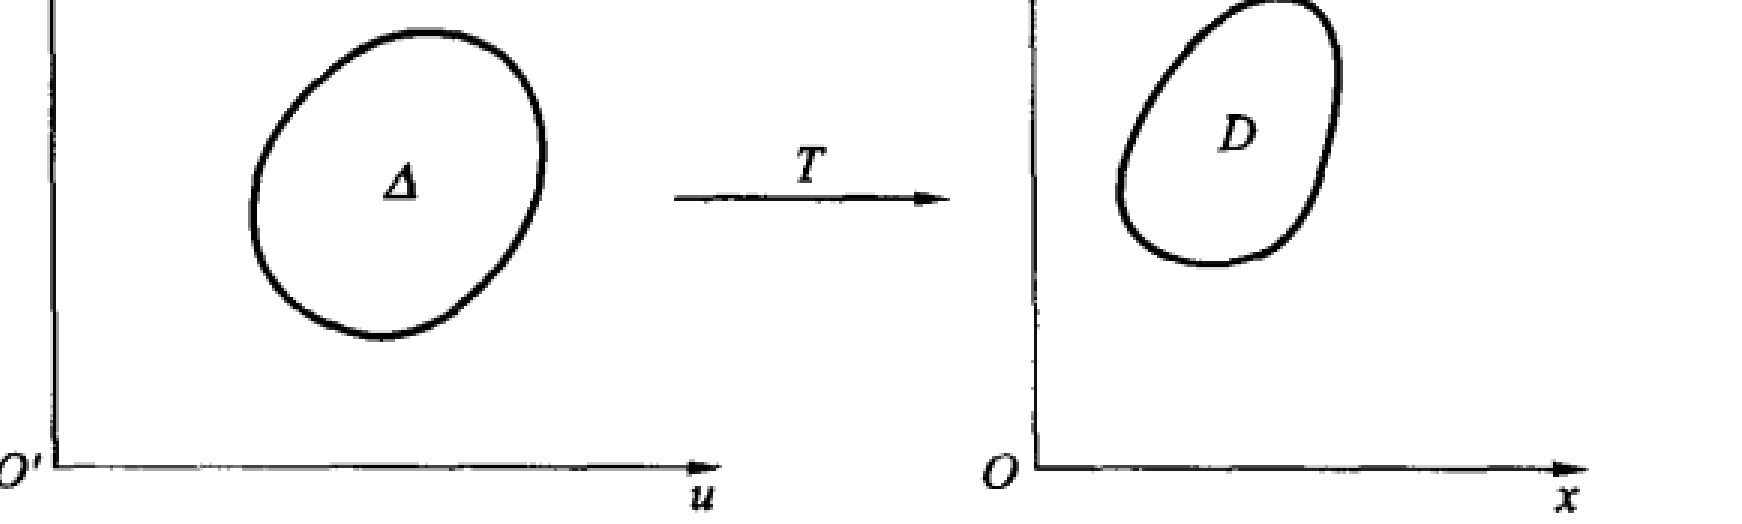
\includegraphics[width=0.72\textwidth]{work/figures/fig20-19}\caption{\relax}\label{fig:20-19}
\end{figure}

假设 $\varphi$，$\psi$ 在 $\Delta$ 有连续的二阶偏导数．显然，重积分换元公式不可能是把\eqref{eq:20-3-2}代入\eqref{eq:20-3-1}得到，因为若把 $\mathrm{d}x$，$\mathrm{d}y$ 看作微分的话，我们根本就不知道
\[
\iint\limits_{\Delta}f\left(\varphi(u,v),\psi(u,v)\right)\left(\frac{\partial\varphi}{\partial u}\mathrm{d}u+\frac{\partial\varphi}{\partial v}\mathrm{d}v\right)\left(\frac{\partial\psi}{\partial u}\mathrm{d}u+\frac{\partial\psi}{\partial v}\mathrm{d}v\right)
\]
表示什么？实际上当时用\eqref{eq:20-3-1}表示重积分，完全是一个记号，并说明没有理由把 $\mathrm{d}x\mathrm{d}y$ 看作是微分的乘积．

下面进一步，假设变换的函数行列式不取零值，即
\[
J(u,v)=\frac{\partial(x,y)}{\partial(u,v)}=\begin{vmatrix}
\dfrac{\partial\varphi}{\partial u} & \dfrac{\partial\varphi}{\partial v}\\[8pt]
\dfrac{\partial\psi}{\partial u} & \dfrac{\partial\psi}{\partial v}
\end{vmatrix}
\]
在 $\Delta$ 内没有零点．由于所有偏导数在 $\Delta$ 连续，因此 $\dfrac{\partial(x,y)}{\partial(u,v)}$ 恒为正或恒为负．

这时 $T\colon\Delta\to D$ 把 $\Delta$ 的内点映为 $D$ 的内点，并且是一一对应的，同时把 $\Delta$ 的边界点映为 $D$ 的边界点．这时，二重积分的变量代换公式是
\[
\iint\limits_{D}f(x,y)\,\mathrm{d}x\mathrm{d}y=\iint\limits_{\Delta}f\left(\varphi(u,v),\psi(u,v)\right)\left|J(u,v)\right|\,\mathrm{d}u\mathrm{d}v.
\]

为证明此公式，先证明下面的引理．

\begin{lemma}\label{lem:20-3-1}
设 $\sigma$ 是 $\Delta$ 内的一个正方形，左下方顶点为 $(u_{0},v_{0})$，边长为 $h$（图~\ref{fig:20-20}），经 $T$ 映为 $D$ 内的一个曲边四边形，记为 $S$，则 $S$ 的面积
\begin{equation}\label{eq:20-3-3}
\left|S\right|=\iint\limits_{\sigma}\left|J(u,v)\right|\,\mathrm{d}u\mathrm{d}v.
\tag{3}
\end{equation}
\end{lemma}

\begin{figure}[htbp]
\centering
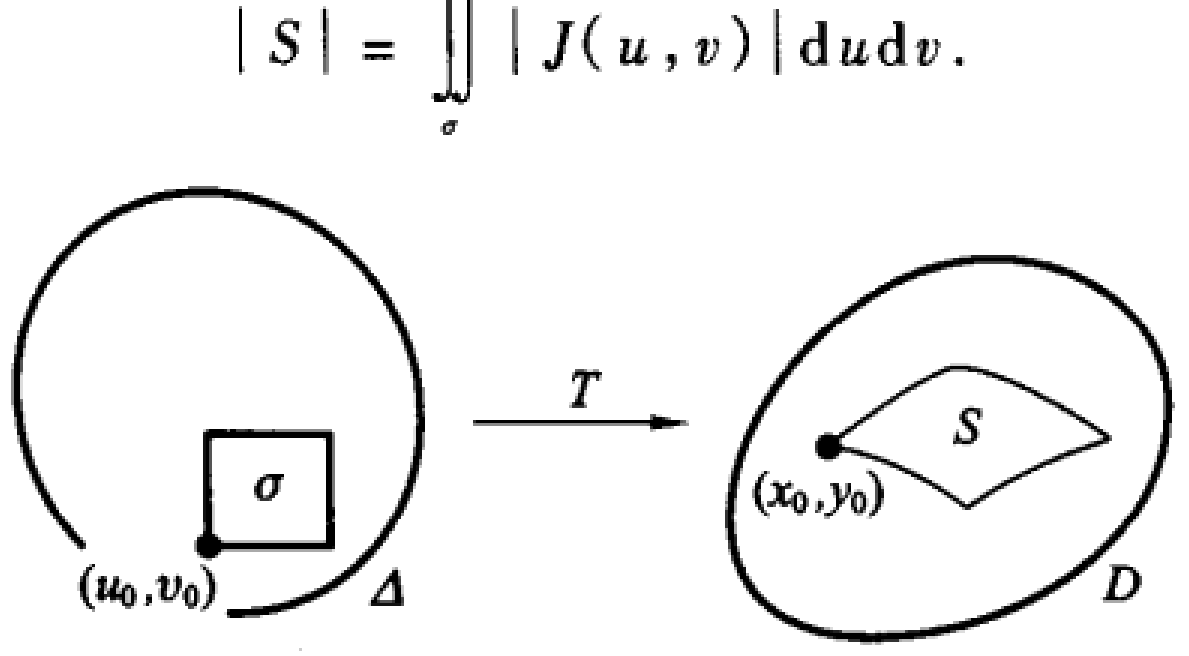
\includegraphics[width=0.55\textwidth]{work/figures/fig20-20}\caption{\relax}\label{fig:20-20}
\end{figure}

\begin{proof}
先设 $J(u,v)>0$．记 $\sigma$ 的边界为 $L$，$S$ 的边界为 $\mathcal{L}$．这时 $\mathcal{L}$ 可以分成四段，第一段的参数方程为
\[
\begin{cases}
x=\varphi(u,v_{0}),\\
y=\psi(u,v_{0}),
\end{cases}
\quad u_{0}\leqslant u\leqslant u_{0}+h,
\]
而第二段的参数方程为
\[
\begin{cases}
x=\varphi(u_{0}+h,v),\\
y=\psi(u_{0}+h,v),
\end{cases}
\quad v_{0}\leqslant v\leqslant v_{0}+h,
\]
其余两段可类似地写出．显然，$\mathcal{L}$ 在每段都是光滑的，因而是逐段光滑的．回忆定积分应用时讲授过的（第八章§2），如果简单逐段光滑闭曲线用参数方程给出，那么它所包围的面积为
\[
\left|S\right|=\frac{1}{2}\int_{\mathcal{L}}x\,\mathrm{d}y-y\,\mathrm{d}x,
\]
其中 $\mathcal{L}$ 的方向取正向．我们先按 $\mathcal{L}$ 是正向进行计算．把 $\mathcal{L}$ 四段的参数方程代入上式，得
\[
\begin{aligned}
2\left|S\right|&=\int_{u_{0}}^{u_{0}+h}\left[\varphi(u,v_{0})\frac{\partial\psi(u,v_{0})}{\partial u}-\psi(u,v_{0})\frac{\partial\varphi(u,v_{0})}{\partial u}\right]\mathrm{d}u+\\
&\ \int_{v_{0}}^{v_{0}+h}\left[\varphi(u_{0}+h,v)\frac{\partial\psi(u_{0}+h,v)}{\partial v}-\right.\\
&\ \left.\psi(u_{0}+h,v)\frac{\partial\varphi(u_{0}+h,v)}{\partial v}\right]\mathrm{d}v+\\
&\ \int_{u_{0}+h}^{u_{0}}\left[\varphi(u,v_{0}+h)\frac{\partial\psi(u,v_{0}+h)}{\partial u}-\right.\\
&\ \left.\psi(u,v_{0}+h)\frac{\partial\varphi(u,v_{0}+h)}{\partial u}\right]\mathrm{d}u+\\
&\ \int_{v_{0}+h}^{v_{0}}\left[\varphi(u_{0},v)\frac{\partial\psi(u_{0},v)}{\partial v}-\psi(u_{0},v)\frac{\partial\varphi(u_{0},v)}{\partial v}\right]\mathrm{d}v.
\end{aligned}
\]
把上面积分内的八项两两配对，并应用微积分基本定理，例如第一个积分的第一项与第三个积分的第一项相加，得
\[
\begin{aligned}
&-\int_{u_{0}}^{u_{0}+h}\left[\varphi(u,v_{0}+h)\frac{\partial\psi(u,v_{0}+h)}{\partial u}-\varphi(u,v_{0})\frac{\partial\psi(u,v_{0})}{\partial u}\right]\mathrm{d}u\\
=&-\int_{u_{0}}^{u_{0}+h}\mathrm{d}u\int_{v_{0}}^{v_{0}+h}\left[\frac{\partial\varphi(u,v)}{\partial v}\frac{\partial\psi(u,v)}{\partial u}+\varphi(u,v)\frac{\partial^{2}\psi(u,v)}{\partial v\partial u}\right]\mathrm{d}v\\
=&-\iint\limits_{\sigma}\left[\frac{\partial\varphi}{\partial v}\frac{\partial\psi}{\partial u}+\varphi\frac{\partial^{2}\psi}{\partial v\partial u}\right]\mathrm{d}u\mathrm{d}v,
\end{aligned}
\]
其中最后一个等式是根据重积分与累次积分的关系得到的．对其余六项同样处理，得
\[
\begin{aligned}
2\left|S\right|&=-\iint\limits_{\sigma}\left[\frac{\partial\varphi}{\partial v}\frac{\partial\psi}{\partial u}+\varphi\frac{\partial^{2}\psi}{\partial v\partial u}\right]\mathrm{d}u\mathrm{d}v+\iint\limits_{\sigma}\left[\frac{\partial\psi}{\partial v}\frac{\partial\varphi}{\partial u}+\psi\frac{\partial^{2}\varphi}{\partial v\partial u}\right]\mathrm{d}u\mathrm{d}v+\\
&\ \iint\limits_{\sigma}\left[\frac{\partial\varphi}{\partial u}\frac{\partial\psi}{\partial v}+\varphi\frac{\partial^{2}\psi}{\partial u\partial v}\right]\mathrm{d}u\mathrm{d}v-\iint\limits_{\sigma}\left[\frac{\partial\psi}{\partial u}\frac{\partial\varphi}{\partial v}+\psi\frac{\partial^{2}\varphi}{\partial u\partial v}\right]\mathrm{d}u\mathrm{d}v\\
&=2\iint\limits_{\sigma}\left|\begin{matrix}\dfrac{\partial\varphi}{\partial u}&\dfrac{\partial\varphi}{\partial v}\\[6pt]
\dfrac{\partial\psi}{\partial u}&\dfrac{\partial\psi}{\partial v}\end{matrix}\right|\mathrm{d}u\mathrm{d}v=2\iint\limits_{\sigma}J(u,v)\,\mathrm{d}u\mathrm{d}v.
\end{aligned}
\]
这时，由 $J(u,v)>0$，知上式右边取正值，与左边的面积连正负号都一致．这说明当初取 $\mathcal{L}$ 是正向的假定是正确的．当 $J(u,v)<0$ 时，作类似的计算，得
\[
2\left|S\right|=-\iint\limits_{\sigma}J(u,v)\,\mathrm{d}u\mathrm{d}v.
\]
总之我们得到了
\[
\left|S\right|=\iint\limits_{\sigma}\left|J(u,v)\right|\,\mathrm{d}u\mathrm{d}v
\]
的结论，这就完成了引理的证明．
\end{proof}

应用积分中值定理，知存在 $(\overline{u},\overline{v})\in\sigma$，使得
\begin{equation}\label{eq:20-3-4}
\left|S\right|=\left|J(\overline{u},\overline{v})\right|\left|\sigma\right|.
\tag{4}
\end{equation}
这个公式，我们是对 $\sigma$ 为正方形时证明的．实际上，当 $\sigma$ 是由逐段光滑闭曲线围成时，公式仍然正确．我们现在先承认这一点，读者以后学了格林公式之后便能更清楚地理解．

由公式\eqref{eq:20-3-4}，可以得到函数行列式的几何解释．事实上，在\eqref{eq:20-3-4}中令 $\sigma$ 的直径趋向于零，从而使 $\sigma$ 收缩为一点 $(u_{0},v_{0})$，由 $J(u,v)$ 的连续性，知
\[
\left|J(u_{0},v_{0})\right|=\lim_{d(\sigma)\to 0}\frac{\left|S\right|}{\left|\sigma\right|},
\]
也就是说，$J(u_{0},v_{0})$ 的绝对值，表示包含 $(u_{0},v_{0})$ 的简单闭曲线 $L$ 所包围的面积 $\left|\sigma\right|$，同 $L$ 在映射 $T$ 下的像 $\mathcal{L}$ 所包围的面积 $\left|S\right|$ 的比的极限，或简单说成是映射 $T$ 在 $(u_{0},v_{0})$ 的面积变化率．为解释其正负号的含义，回忆引~\ref{lem:20-3-1} 证明的过程，我们计算 $\left|\sigma\right|$ 与 $\left|S\right|$ 时，积分的顺序都是按 $L$ 与 $\mathcal{L}$ 的正向进行的，这时假定 $J(u,v)$ 为正，算出来的结果连正负号都是对的．因此，$J(u_{0},v_{0})>0$，表示在 $(u_{0},v_{0})$ 附近包含 $(u_{0},v_{0})$ 的闭曲线 $L$，在映射 $T$ 下的像 $\mathcal{L}$，它们是同向的（即 $L$ 取正向，$\mathcal{L}$ 也取正向；$L$ 取反向，$\mathcal{L}$ 也取反向）．而 $J(u_{0},v_{0})<0$ 则表示 $L$ 与 $\mathcal{L}$ 的方向是相反的（即若 $L$ 取正向，则 $\mathcal{L}$ 取反向；若 $L$ 取反向，则 $\mathcal{L}$ 取正向）．在这个意义下，把 $J(u,v)$ 看成微商概念在二维平面间的映射的推广是合理的．

现在，我们可以来证明二重积分的变量代换公式了．

\begin{theorem}\label{thm:20-3}
设变换 $T$：
\[
\begin{cases}
x=\varphi(u,v),\\
y=\psi(u,v)
\end{cases}
\]
把 $Ouv$ 平面上由逐段光滑的闭曲线围成的区域 $\Delta$ 一一地映射为 $Oxy$ 平面的区域 $D$，且 $\varphi$，$\psi$ 在 $\Delta$ 有二阶连续偏导数，
\[
J(u,v)=\frac{\partial(x,y)}{\partial(u,v)}\neq 0\quad\text{当}\ (u,v)\in\Delta,
\]
而 $f(x,y)$ 是定义在 $D$ 上的连续函数，则
\[
\iint_{D}f(x,y)\,\mathrm{d}x\mathrm{d}y=\iint_{\Delta}f\left(\varphi(u,v),\psi(u,v)\right)\left|J(u,v)\right|\,\mathrm{d}u\mathrm{d}v.
\]
\end{theorem}

\begin{proof}
用间隔为 $h$ 的平行于坐标轴的直线网，作 $\Delta$ 的一个分法：$\Delta\sigma_{1}$，$\Delta\sigma_{2}$，$\cdots$，$\Delta\sigma_{n}$，则通过映射 $T$ 便对应于 $D$ 的一个分法：$\Delta S_{1}$，$\Delta S_{2}$，$\cdots$，$\Delta S_{n}$．由公式\eqref{eq:20-3-4}知，存在 $(\bar{u}_{i},\bar{v}_{i})\in\Delta\sigma_{i}$，使得
\[
\left|\Delta S_{i}\right|=\left|J(\bar{u}_{i},\bar{v}_{i})\right|\left|\Delta\sigma_{i}\right|.
\]
记
\[
\begin{cases}
\bar{x}_{i}=\varphi(\bar{u}_{i},\bar{v}_{i}),\\
\bar{y}_{i}=\psi(\bar{u}_{i},\bar{v}_{i}),
\end{cases}
\]
显然 $(\bar{x}_{i},\bar{y}_{i})\in\Delta S_{i}$．作黎曼和
\[
\begin{aligned}
\sum_{i=1}^{n}f(\bar{x}_{i},\bar{y}_{i})\left|\Delta S_{i}\right|&=\sum_{i=1}^{n}f\left(\varphi(\bar{u}_{i},\bar{v}_{i}),\psi(\bar{u}_{i},\bar{v}_{i})\right)\left|\Delta S_{i}\right|\\
&=\sum_{i=1}^{n}f\left(\varphi(\bar{u}_{i},\bar{v}_{i}),\psi(\bar{u}_{i},\bar{v}_{i})\right)\left|J(\bar{u}_{i},\bar{v}_{i})\right|\left|\Delta\sigma_{i}\right|.
\end{aligned}
\]

\begin{figure}[htbp]
\centering
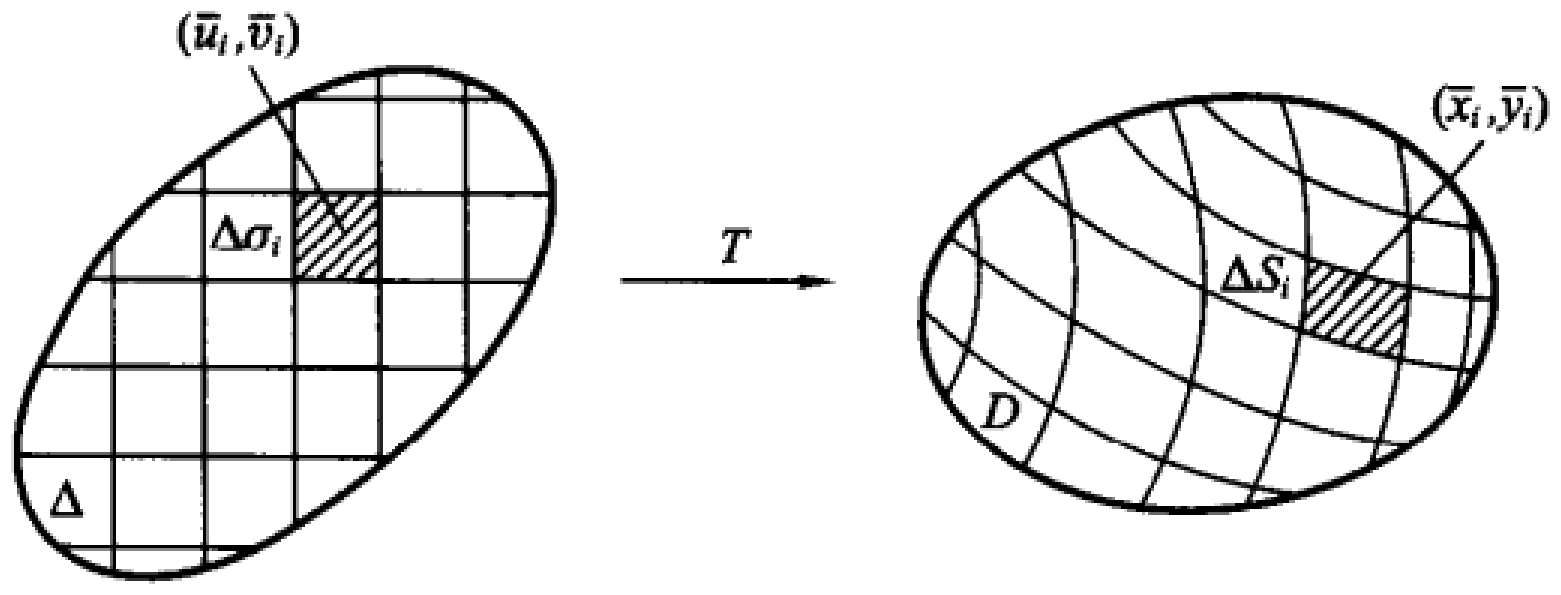
\includegraphics[width=0.68\textwidth]{work/figures/fig20-21}\caption{\relax}\label{fig:20-21}
\end{figure}

令 $h\to 0$，这时 $\lambda=\max\left(d(\Delta S_{i})\right)\to 0$，在上式两边取极限，便得
\[
\iint_{D}f(x,y)\,\mathrm{d}x\mathrm{d}y=\iint_{\Delta}f\left(\varphi(u,v),\psi(u,v)\right)\left|J(u,v)\right|\,\mathrm{d}u\mathrm{d}v.
\]
定理~\ref{thm:20-3}证完．
\end{proof}

从微元的观点来看，这公式是比较容易理解的．事实上，公式可以写成
\[
\iint_{D}f(x,y)\,\mathrm{d}S=\iint_{\Delta}f\left(\varphi(u,v),\psi(u,v)\right)\left|J(u,v)\right|\,\mathrm{d}\sigma.
\]
用平行于坐标轴的直线网作 $\Delta$ 的分法，相应地得到 $D$ 的用曲线网作成的分法，这时 $D$ 上的面积微元 $\mathrm{d}S$ 与 $\Delta$ 的面积微元 $\mathrm{d}\sigma$ 之间，按引理~\ref{lem:20-3-1}，有下列的关系
\begin{equation}\label{eq:20-3-5}
\mathrm{d}S=\left|J(u,v)\right|\mathrm{d}\sigma,
\tag{5}
\end{equation}
因此，相应地两边对 $f(P)$ 积分便得上述的换元公式．在这意义下，符号
\[
\iint_{D}f(P)\,\mathrm{d}S=\iint_{\Delta}f\left(\varphi(Q),\psi(Q)\right)\left|J(Q)\right|\,\mathrm{d}\sigma
\]
更能反映出变量代换中函数行列式是面积元之比的直观意义，但缺点是看不到积分变量，故通常还是写作
\[
\iint_{D}f(x,y)\,\mathrm{d}x\mathrm{d}y=\iint_{\Delta}f\left(\varphi(u,v),\psi(u,v)\right)\left|J(u,v)\right|\,\mathrm{d}u\mathrm{d}v,
\]
只要读者把
\[
\mathrm{d}x\mathrm{d}y=\left|J(u,v)\right|\mathrm{d}u\mathrm{d}v
\]
理解为\eqref{eq:20-3-5}的一种写法即可．

\begin{example}\label{ex:20-3-1}
计算二重积分
\[
\iint\limits_{D}xy\,\mathrm{d}x\mathrm{d}y,
\]
其中 $D$ 是由抛物线 $y^{2}=x$，$y^{2}=4x$，$x^{2}=y$，$x^{2}=4y$ 所围成的区域．
\end{example}

\begin{proof}[解]
画出 $D$ 的图形，根据 $D$ 的特点，作变换

\begin{figure}[htbp]
\centering
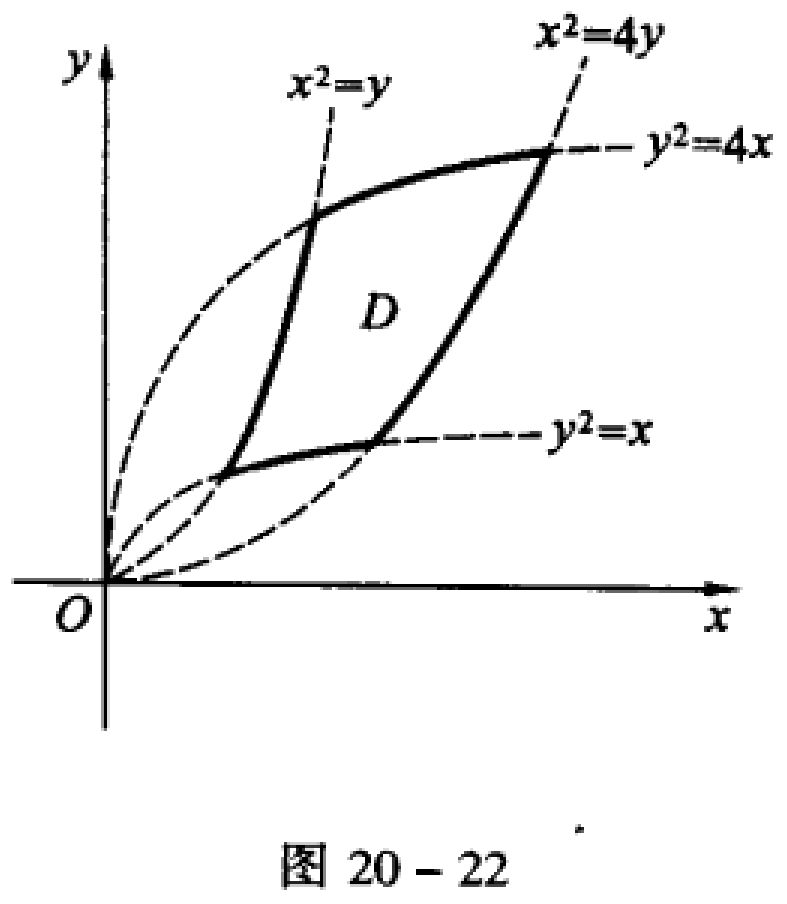
\includegraphics[width=0.30\textwidth]{work/figures/fig20-22}\caption{\relax}\label{fig:20-22}
\end{figure}
\[
T^{-1}:\quad u=\frac{y^{2}}{x},\quad v=\frac{x^{2}}{y},
\]
它把 $D$ 一一地映为正方形区域 $\Delta$：$1\leqslant u\leqslant 4$，$1\leqslant v\leqslant 4$．

计算
\[
\frac{\partial(u,v)}{\partial(x,y)}=\begin{vmatrix}
-\dfrac{y^{2}}{x^{2}} & \dfrac{2y}{x}\\[8pt]
\dfrac{2x}{y} & -\dfrac{x^{2}}{y^{2}}
\end{vmatrix}=-3.
\]
由于

\begin{figure}[htbp]
\centering
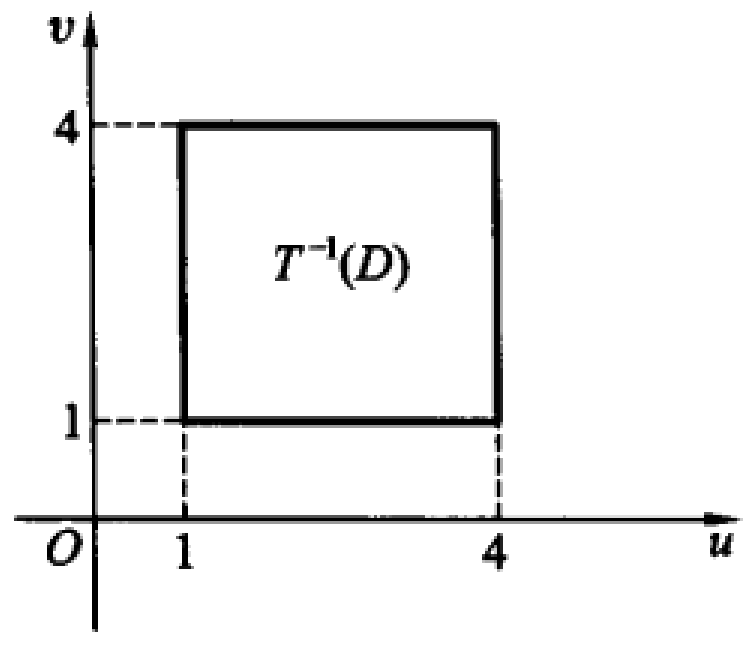
\includegraphics[width=0.28\textwidth]{work/figures/fig20-23}\caption{\relax}\label{fig:20-23}
\end{figure}
\[
\frac{\partial(x,y)}{\partial(u,v)}\cdot\frac{\partial(u,v)}{\partial(x,y)}=1,
\]
知
\[
\left|J(u,v)\right|=\left|\frac{\partial(x,y)}{\partial(u,v)}\right|=\frac{1}{3}.
\]
而
\[
uv=\frac{y^{2}}{x}\cdot\frac{x^{2}}{y}=xy,
\]
因此
\[
\iint_{D}xy\,\mathrm{d}x\mathrm{d}y=\iint_{\Delta}uv\cdot\frac{1}{3}\,\mathrm{d}u\mathrm{d}v=\frac{1}{3}\int_{1}^{4}u\,\mathrm{d}u\int_{1}^{4}v\,\mathrm{d}v=\frac{75}{4}.
\]
\end{proof}

平面变量代换中最重要的一种是\emph{极坐标变换}：
\[
\begin{cases}
x=r\cos\theta,\\
y=r\sin\theta.
\end{cases}
\]
变换的函数行列式为
\[
\frac{\partial(x,y)}{\partial(r,\theta)}=\begin{vmatrix}
\cos\theta & -r\sin\theta\\
\sin\theta & r\cos\theta
\end{vmatrix}=r.
\]
这个变换使 $Oxy$ 平面以原点为心的圆变为 $Or\theta$ 平面的直线 $r=$ 常数，把 $Oxy$ 平面的射线变为 $Or\theta$ 平面的另一束直线 $\theta=$ 常数．因此，极坐标变换对 $D$ 为由圆周与射线围成的区域时比较有效．由于这时 $r$，$\theta$ 的几何意义比较明显，我们有时很容易便写出 $Or\theta$ 平面区域的积分限，而无需把 $\Delta$ 画出来．

\begin{example}\label{ex:20-3-2}
计算
\[
\iint_{D}\mathrm{e}^{-x^{2}-y^{2}}\,\mathrm{d}x\mathrm{d}y,
\]
其中 $D$ 由 $x$，$y$ 正半轴与单位圆周及半径为 $2$ 的同心圆围成．
\end{example}

\begin{proof}[解]
作极坐标变换
\[
\begin{cases}
x=r\cos\theta,\\
y=r\sin\theta.
\end{cases}
\]
从 $r$，$\theta$ 的几何意义立刻看出，对应于 $D$ 的 $r$，$\theta$ 为

\begin{figure}[htbp]
\centering
\begin{tikzpicture}[scale=1.15,baseline=(current bounding box.center)]
  \fill[gray!12] (0.85,0) arc (0:90:0.85) -- (0,2) arc (90:0:2) -- cycle;
  \draw[{-Latex}] (-0.25,0) -- (2.5,0) node[below left] {$x$};
  \draw[{-Latex}] (0,-0.25) -- (0,2.5) node[below left] {$y$};
  \draw (0.85,0) arc (0:90:0.85);
  \draw (2,0) arc (0:90:2);
  \node at (1.25,0.95) {$D$};
  \node[below] at (0.85,0) {$1$};
  \node[below] at (2,0) {$2$};
\end{tikzpicture}\caption{\relax}\label{fig:20-24}
\end{figure}
\[
1\leqslant r\leqslant 2,\quad 0\leqslant\theta\leqslant\frac{\pi}{2}.
\]
因此
\[
\begin{aligned}
\iint_{D}\mathrm{e}^{-x^{2}-y^{2}}\,\mathrm{d}x\mathrm{d}y&=\int_{0}^{\frac{\pi}{2}}\mathrm{d}\theta\int_{1}^{2}\mathrm{e}^{-r^{2}}r\,\mathrm{d}r\\
&=\frac{\pi}{2}\int_{1}^{2}r\mathrm{e}^{-r^{2}}\,\mathrm{d}r=-\frac{\pi}{4}\mathrm{e}^{-r^{2}}\bigg|_{1}^{2}=\frac{\pi}{4}\left(\mathrm{e}^{-1}-\mathrm{e}^{-4}\right).
\end{aligned}
\]
\end{proof}

回忆定理~\ref{thm:20-3} 的证明，对极坐标变换来说，在公式
\begin{equation}\label{eq:20-3-6}
\iint\limits_{D}f(x,y)\,\mathrm{d}x\mathrm{d}y=\iint\limits_{\Delta}f\left(r\cos\theta,r\sin\theta\right)r\,\mathrm{d}r\mathrm{d}\theta
\tag{6}
\end{equation}
的证明中，对 $D$ 实际上是用 $\theta=$ 常数与 $r=$ 常数的两束曲线作分法（图~\ref{fig:20-25}）．从微元法的观点来看，这时的面积微元为（图~\ref{fig:20-26}）

\begin{figure}[htbp]
\centering
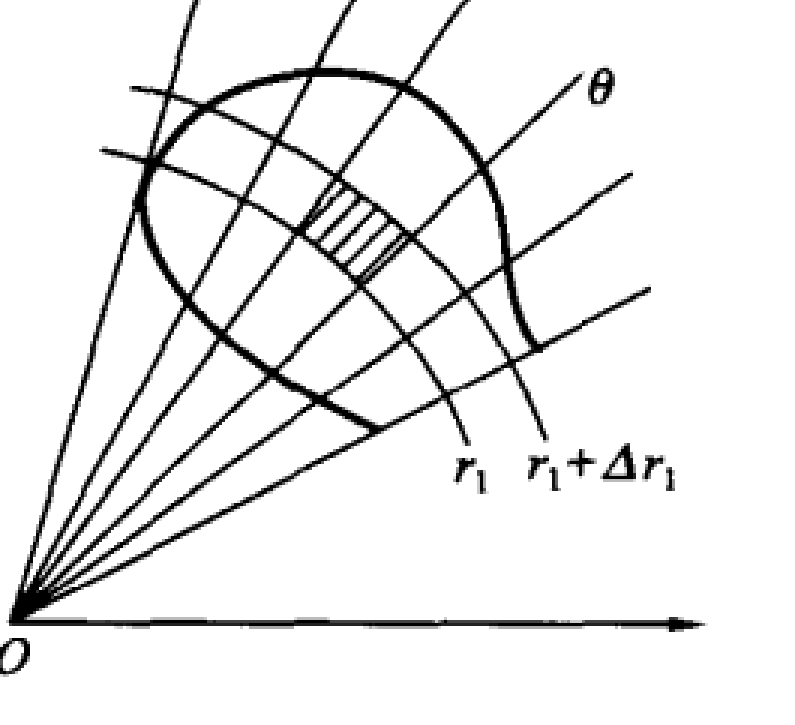
\includegraphics[width=0.30\textwidth]{work/figures/fig20-25}\caption{\relax}\label{fig:20-25}
\end{figure}

\begin{figure}[htbp]
\centering
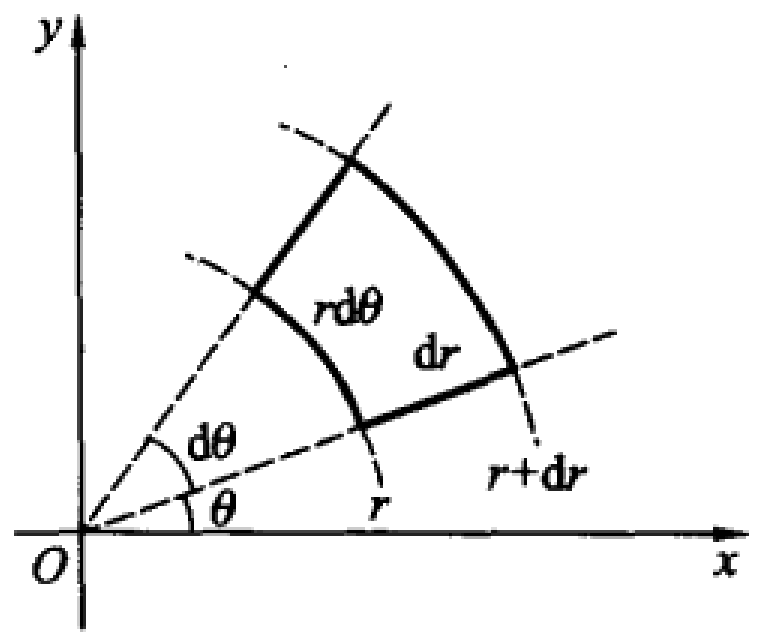
\includegraphics[width=0.30\textwidth]{work/figures/fig20-26}\caption{\relax}\label{fig:20-26}
\end{figure}
\[
\mathrm{d}S=r\,\mathrm{d}r\mathrm{d}\theta,
\]
因此，$D$ 上的函数 $f(x,y)$ 的积分自然应该等于微元
\[
f(r\cos\theta,r\sin\theta)\,r\,\mathrm{d}r\mathrm{d}\theta
\]
之和，这就是公式\eqref{eq:20-3-6}．

\begin{example}\label{ex:20-3-3}
利用二重积分变量代换计算概率积分
\[
\int_{0}^{+\infty}\mathrm{e}^{-x^{2}}\,\mathrm{d}x.
\]
\end{example}

\begin{proof}[解]
已知
\[
\int_{0}^{+\infty}\mathrm{e}^{-x^{2}}\,\mathrm{d}x=\lim_{a\to+\infty}\int_{0}^{a}\mathrm{e}^{-x^{2}}\,\mathrm{d}x.
\]
而
\[
\left(\int_{0}^{a}\mathrm{e}^{-x^{2}}\,\mathrm{d}x\right)^{2}=\int_{0}^{a}\mathrm{e}^{-x^{2}}\,\mathrm{d}x\int_{0}^{a}\mathrm{e}^{-y^{2}}\,\mathrm{d}y=\iint\limits_{D_{a}}\mathrm{e}^{-x^{2}-y^{2}}\,\mathrm{d}x\mathrm{d}y,
\]
其中 $D_{a}=[0,a]\times[0,a]$，右边的积分仍无法计算，引入
\[
\overline{D}_{a}=\left\{(x,y)\mid x^{2}+y^{2}\leqslant a^{2},x\geqslant 0,y\geqslant 0\right\},
\]
\[
\overline{\overline{D}}_{a}=\left\{(x,y)\mid x^{2}+y^{2}\leqslant 2a^{2},x\geqslant 0,y\geqslant 0\right\},
\]
则 $\overline{D}_{a}\subset D_{a}\subset\overline{\overline{D}}_{a}$．因为 $\mathrm{e}^{-x^{2}-y^{2}}\geqslant 0$，
\begin{equation}\label{eq:20-3-7}
\iint\limits_{\overline{D}_{a}}\mathrm{e}^{-x^{2}-y^{2}}\,\mathrm{d}x\mathrm{d}y\leqslant\iint\limits_{D_{a}}\mathrm{e}^{-x^{2}-y^{2}}\,\mathrm{d}x\mathrm{d}y\leqslant\iint\limits_{\overline{\overline{D}}_{a}}\mathrm{e}^{-x^{2}-y^{2}}\,\mathrm{d}x\mathrm{d}y.
\tag{7}
\end{equation}

\begin{figure}[htbp]
\centering
\begin{tikzpicture}[scale=1.05,baseline=(current bounding box.center)]
  \draw[{-Latex}] (-0.25,0) -- (2.6,0) node[below left] {$x$};
  \draw[{-Latex}] (0,-0.25) -- (0,2.6) node[below left] {$y$};
  \draw (0,2.2) -- (2.2,2.2) -- (2.2,0);
  \draw (1.556,0) arc (0:90:1.556);
  \draw (2.2,0) arc (0:90:2.2);
  \node[right] at (0.1,2.1) {\small $\overline{\overline{D}}_{a}$};
  \node at (1.35,1.35) {\small $D_{a}$};
  \node at (0.75,0.75) {\small $\overline{D}_{a}$};
  \node[below] at (1.556,0) {$a$};
  \node[below] at (2.2,0) {$\sqrt{2}\,a$};
\end{tikzpicture}\caption{\relax}\label{fig:20-27}
\end{figure}

而对不等式前后的两个积分，可以用极坐标变换计算
\[
\iint\limits_{\overline{D}_{a}}\mathrm{e}^{-x^{2}-y^{2}}\,\mathrm{d}x\mathrm{d}y=\int_{0}^{\frac{\pi}{2}}\mathrm{d}\theta\int_{0}^{a}r\mathrm{e}^{-r^{2}}\,\mathrm{d}r=\frac{\pi}{4}(1-\mathrm{e}^{-a^{2}}),
\]
\[
\iint\limits_{\overline{\overline{D}}_{a}}\mathrm{e}^{-x^{2}-y^{2}}\,\mathrm{d}x\mathrm{d}y=\frac{\pi}{4}(1-\mathrm{e}^{-2a^{2}}).
\]
代入\eqref{eq:20-3-7}中再令 $a\to+\infty$，用极限的夹逼定理，得
\[
\lim_{a\to+\infty}\iint_{D_{a}}\mathrm{e}^{-x^{2}-y^{2}}\,\mathrm{d}x\mathrm{d}y=\frac{\pi}{4},
\]
因此
\[
\int_{0}^{+\infty}\mathrm{e}^{-x^{2}}\,\mathrm{d}x=\frac{\sqrt{\pi}}{2}.
\]
\end{proof}

在第十九章 §2 中我们用无穷积分交换顺序计算过这个积分．显然，这里的计算要简便得多．

在上面计算积分
\[
\iint\limits_{\overline{D}_{a}}\mathrm{e}^{-x^{2}-y^{2}}\,\mathrm{d}x\mathrm{d}y
\]
的过程中，用了极坐标变换
\[
\begin{cases}
x=r\cos\theta,\\
y=r\sin\theta,
\end{cases}
\quad 0\leqslant\theta\leqslant\frac{\pi}{2},\ 0\leqslant r\leqslant a.
\]
这时函数行列式
\[
J(r,\theta)=r.
\]
在 $r=0$ 时为 $0$，不满足定理~\ref{thm:20-3} 的条件．而事实上，我们的计算仍然是正确的，它可以解释如下：用小扇形把原点挖去，引入区域
\[
D_{a\varepsilon}=\left\{(x,y)\mid\varepsilon^{2}\leqslant x^{2}+y^{2}\leqslant a^{2},x\geqslant 0,y\geqslant 0\right\},
\]

\begin{figure}[htbp]
\centering
\begin{tikzpicture}[scale=1.1,baseline=(current bounding box.center)]
  \draw[{-Latex}] (-0.25,0) -- (2.5,0) node[below left] {$x$};
  \draw[{-Latex}] (0,-0.25) -- (0,2.3) node[below left] {$y$};
  \draw (2,0) arc (0:90:2);
  \draw (0.35,0) arc (0:90:0.35);
  \fill[gray!12] (2,0) arc (0:90:2) -- (0,2) -- (0,0.35) arc (90:0:0.35) -- (0.35,0) -- cycle;
  \node at (1.1,1.1) {$D_{a\varepsilon}$};
  \node[below] at (0.35,0) {$\varepsilon$};
  \node[below] at (2,0) {$a$};
\end{tikzpicture}\caption{\relax}\label{fig:20-28}
\end{figure}

则 $J(r,\theta)$ 在 $D_{a\varepsilon}$ 不为 $0$，这时
\[
\begin{aligned}
\iint\limits_{\overline{D}_{a}}\mathrm{e}^{-x^{2}-y^{2}}\,\mathrm{d}x\mathrm{d}y&=\lim_{\varepsilon\to 0}\iint\limits_{D_{a\varepsilon}}\mathrm{e}^{-x^{2}-y^{2}}\,\mathrm{d}x\mathrm{d}y\\
&=\lim_{\varepsilon\to 0}\int_{0}^{\frac{\pi}{2}}\mathrm{d}\theta\int_{\varepsilon}^{a}r\mathrm{e}^{-r^{2}}\,\mathrm{d}r=\lim_{\varepsilon\to 0}\frac{\pi}{4}\left(\mathrm{e}^{-\varepsilon^{2}}-\mathrm{e}^{-a^{2}}\right)\\
&=\frac{\pi}{4}(1-\mathrm{e}^{-a^{2}}).
\end{aligned}
\]
至于在第一个等式中，左边等于右边的极限，是因为二者之差
\[
\iint_{\overline{D}_{a}\setminus D_{a\varepsilon}}\mathrm{e}^{-x^{2}-y^{2}}\,\mathrm{d}x\mathrm{d}y\leqslant\iint_{\overline{D}_{a}\setminus D_{a\varepsilon}}\mathrm{d}x\mathrm{d}y\leqslant\frac{\pi}{4}\varepsilon^{2}\to 0\quad(\varepsilon\to 0).
\]

从上述的证明看出，定理~\ref{thm:20-3} 中 $J(u,v)$ 在 $D$ 恒正或恒负的条件可减弱为 $J(u,v)\geqslant 0$，但只允许在 $\Delta$ 的有限个点上取 $0$ 值．事实上，这时可用有限个小圆把这些点挖去，再令这些圆的半径趋向于 $0$ 取极限．

\begin{example}\label{ex:20-3-4}
计算在旋转抛物面 $z=x^{2}+y^{2}$ 之下，$Oxy$ 平面 $z=0$ 之上，由圆柱面
\[
(x-a)^{2}+y^{2}=a^{2}
\]
截出的空间立体的体积．
\end{example}

\begin{proof}[解]
记平面区域
\[
D=\left\{(x,y)\mid(x-a)^{2}+y^{2}\leqslant a^{2}\right\},
\]
我们要计算的体积等于二重积分
\[
V=\iint\limits_{D}(x^{2}+y^{2})\,\mathrm{d}x\mathrm{d}y.
\]

\begin{figure}[htbp]
\centering
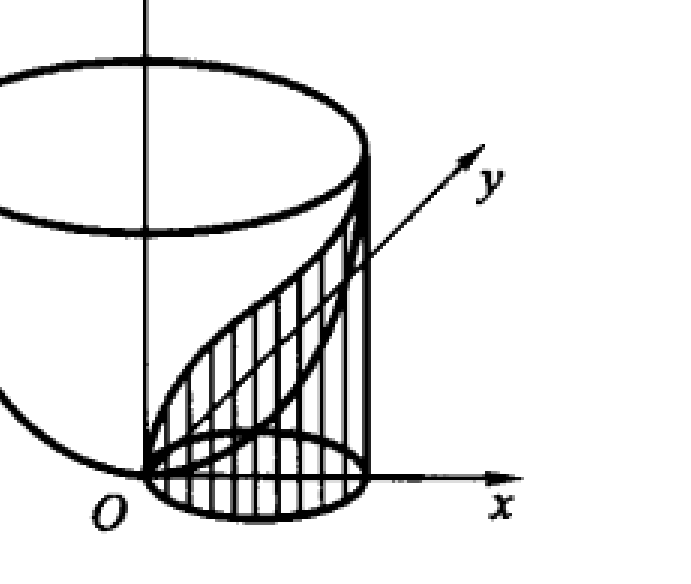
\includegraphics[width=0.30\textwidth]{work/figures/fig20-29}\caption{\relax}\label{fig:20-29}
\end{figure}

作极坐标变换
\[
\begin{cases}
x=r\cos\theta,\\
y=r\sin\theta.
\end{cases}
\]
这时对应于 $D$ 的极坐标（见图~\ref{fig:20-30}）为
\[
-\frac{\pi}{2}\leqslant\theta\leqslant\frac{\pi}{2},\quad 0\leqslant r\leqslant 2a\cos\theta.
\]

\begin{figure}[htbp]
\centering
\begin{tikzpicture}[scale=1.1,baseline=(current bounding box.center)]
  \draw[{-Latex}] (-1.1,0) -- (2.6,0) node[below left] {$x$};
  \draw[{-Latex}] (0,-1.1) -- (0,1.9) node[below left] {$y$};
  \draw (1,0) circle (1);
  \draw[thick] (0,0) -- (60:2) node[above right] {\small $\theta$};
  \node[below] at (2,0) {$2a$};
  \node[above] at (0.5,0.85) {$D$};
\end{tikzpicture}\caption{\relax}\label{fig:20-30}
\end{figure}

因此
\[
\begin{aligned}
\iint_{D}(x^{2}+y^{2})\,\mathrm{d}x\mathrm{d}y&=\int_{-\frac{\pi}{2}}^{\frac{\pi}{2}}\mathrm{d}\theta\int_{0}^{2a\cos\theta}r^{3}\,\mathrm{d}r\\
&=\int_{-\frac{\pi}{2}}^{\frac{\pi}{2}}\frac{1}{4}(2a\cos\theta)^{4}\,\mathrm{d}\theta\\
&=8a^{4}\int_{0}^{\frac{\pi}{2}}\cos^{4}\theta\,\mathrm{d}\theta=8a^{4}\cdot\frac{3\cdot 1}{4\cdot 2}\cdot\frac{\pi}{2}\\
&=\frac{3}{2}\pi a^{4}.
\end{aligned}
\]
\end{proof}

\begin{example}\label{ex:20-3-5}
求椭球体的体积 $V$．
\end{example}

\begin{proof}[解]
设椭球体为
\[
\frac{x^{2}}{a^{2}}+\frac{y^{2}}{b^{2}}+\frac{z^{2}}{c^{2}}\leqslant 1.
\]
则由对称性知

\begin{figure}[htbp]
\centering
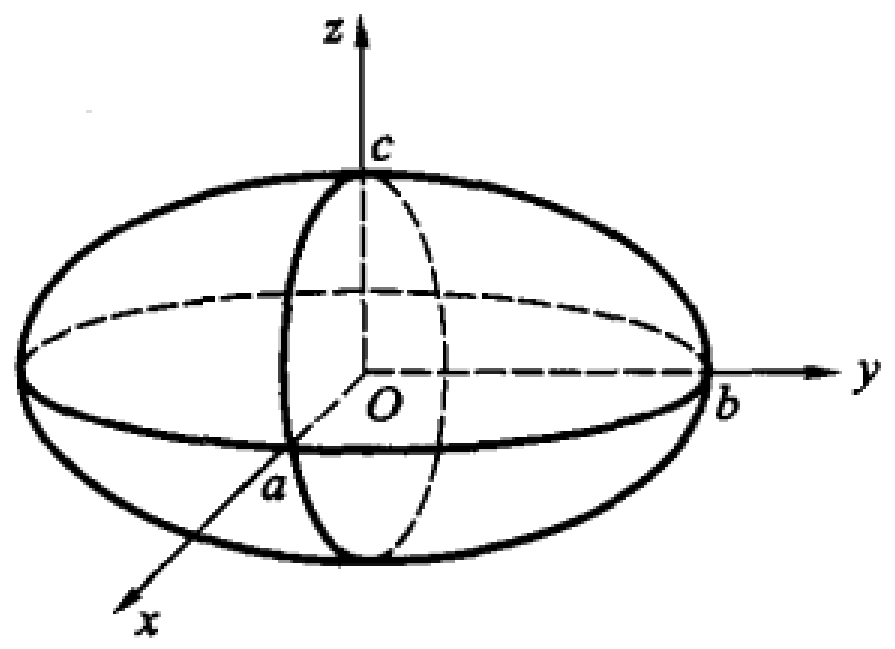
\includegraphics[width=0.34\textwidth]{work/figures/fig20-31}\caption{\relax}\label{fig:20-31}
\end{figure}
\[
V=2\iint_{D}c\sqrt{1-\frac{x^{2}}{a^{2}}-\frac{y^{2}}{b^{2}}}\,\mathrm{d}x\mathrm{d}y,
\]
其中
\[
D=\left\{(x,y)\mid\frac{x^{2}}{a^{2}}+\frac{y^{2}}{b^{2}}\leqslant 1\right\}.
\]
作广义极坐标变换
\[
x=ar\cos\theta,\quad y=br\sin\theta,
\]
则 $D$ 对应于 $0\leqslant r\leqslant 1$，$0\leqslant\theta\leqslant 2\pi$．而
\[
\frac{\partial(x,y)}{\partial(r,\theta)}=\begin{vmatrix}
a\cos\theta & -a\sin\theta\\
b\sin\theta & br\cos\theta
\end{vmatrix}=abr,
\]
因此
\[
\begin{aligned}
V&=2\int_{0}^{2\pi}\mathrm{d}\theta\int_{0}^{1}c\sqrt{1-r^{2}}\,abr\,\mathrm{d}r\\
&=4\pi abc\int_{0}^{1}\sqrt{1-r^{2}}\,r\,\mathrm{d}r=4\pi abc\cdot\frac{1}{2}\cdot\frac{2}{3}\left(1-r^{2}\right)^{\frac{3}{2}}\bigg|_{1}^{0}\\
&=\frac{4}{3}\pi abc.
\end{aligned}
\]
这比在直角坐标系下化累次积分计算要简单得多．
\end{proof}

\subsection{三重积分的变量代换}

三重积分的变量代换公式与二重积分变量代换公式完全类似．我们不再详细推导，在此仅给出公式的叙述．

设函数 $f(x,y,z)$ 在由逐片光滑曲面围成的闭区域 $V$ 上连续，变换 $T$
\[
\begin{cases}
x=x(u,v,w),\\
y=y(u,v,w),\\
z=z(u,v,w)
\end{cases}
\]
将 $Ouvw$ 坐标系下的区域 $\Omega$ 一一映射为 $V$．函数 $x(u,v,w)$，$y(u,v,w)$，$z(u,v,w)$ 在 $\Omega$ 有连续的二阶偏导数，且雅可比行列式
\[
J(u,v,w)=\frac{\partial(x,y,z)}{\partial(u,v,w)}\neq 0,
\]
则
\begin{equation}\label{eq:20-3-8}
\begin{aligned}
&\iiint\limits_{V}f(x,y,z)\,\mathrm{d}x\mathrm{d}y\mathrm{d}z\\
=&\iiint\limits_{\Omega}f\left(x(u,v,w),y(u,v,w),z(u,v,w)\right)\left|\frac{\partial(x,y,z)}{\partial(u,v,w)}\right|\mathrm{d}u\mathrm{d}v\mathrm{d}w.
\end{aligned}
\tag{8}
\end{equation}

公式的证明完全类似于二重积分的情形．即首先证明，函数行列式的大小 $\left|J(u_{0},v_{0},w_{0})\right|$ 实际上就是变换 $T$ 在 $(u_{0},v_{0},w_{0})$ 的体积变化率
\[
\left|J(u_{0},v_{0},w_{0})\right|=\lim\frac{\left|\Delta V\right|}{\Delta\Omega},
\]
其中 $\Delta\Omega$ 是包含 $(u_{0},v_{0},w_{0})$ 的小块体积，$\Delta V$ 是 $\Delta\Omega$ 在变换 $T$ 下的像，而极限过程是 $\Delta\Omega$ 收缩到点 $(u_{0},v_{0},w_{0})$．其次，是用 $u=$ 常数，$v=$ 常数与 $w=$ 常数的三组平行于坐标平面的平面作 $\Omega$ 的分法，这对应于用三束坐标曲面作 $V$ 的分法．这时
\[
\left|J(u,v,w)\right|\mathrm{d}u\mathrm{d}v\mathrm{d}w
\]
就是曲面坐标下的体积元，从而得到公式\eqref{eq:20-3-8}．

一般地，类似于二重积分，如果在有限个点，或有限条光滑曲线，或有限块光滑曲面上 $\dfrac{\partial(x,y,z)}{\partial(u,v,w)}=0$，而在 $V$ 的其余地方 $J(u,v,w)$ 不变号，则变量代换公式仍然成立．

三重积分最常用的变量代换有\emph{柱坐标变换}和\emph{球坐标变换}．分别介绍如下．

（1）柱坐标变换
\[
\begin{cases}
x=r\cos\theta, & 0\leqslant r<+\infty,\\
y=r\sin\theta, & 0\leqslant\theta<2\pi,\\
z=z, & -\infty<z<+\infty,
\end{cases}
\]
这时
\[
J(r,\theta,z)=\frac{\partial(x,y,z)}{\partial(r,\theta,z)}=\begin{vmatrix}
\cos\theta & -r\sin\theta & 0\\
\sin\theta & r\cos\theta & 0\\
0 & 0 & 1
\end{vmatrix}=r.
\]
因此变量代换公式为
\[
\iiint\limits_{V}f(x,y,z)\,\mathrm{d}x\mathrm{d}y\mathrm{d}z=\iiint\limits_{\Omega}f(r\cos\theta,r\sin\theta,z)\,r\,\mathrm{d}r\mathrm{d}\theta\mathrm{d}z.
\]

下面从微元的观点来看看这个公式．在 $Oxyz$ 空间中，柱坐标中的 $r$ 表示 $(x,y,z)$ 在 $Oxy$ 平面上的投影点 $P$ 与原点的距离，而 $\theta$ 则表原点和投影点 $P$ 连线 $OP$ 与 $x$ 轴正向的夹角．坐标曲面 $r=$ 常数是以 $z$ 轴为中心的圆柱面；$\theta=$ 常数是过 $z$ 轴的半平面；$z=$ 常数是垂直于 $z$ 轴的平面（图~\ref{fig:20-32}）．显然如果 $(x,y,z)$ 的柱坐标是 $(r,\theta,z)$，则 $(r,\theta)$ 就是 $(x,y)$ 的极坐标．

\begin{figure}[htbp]
\centering
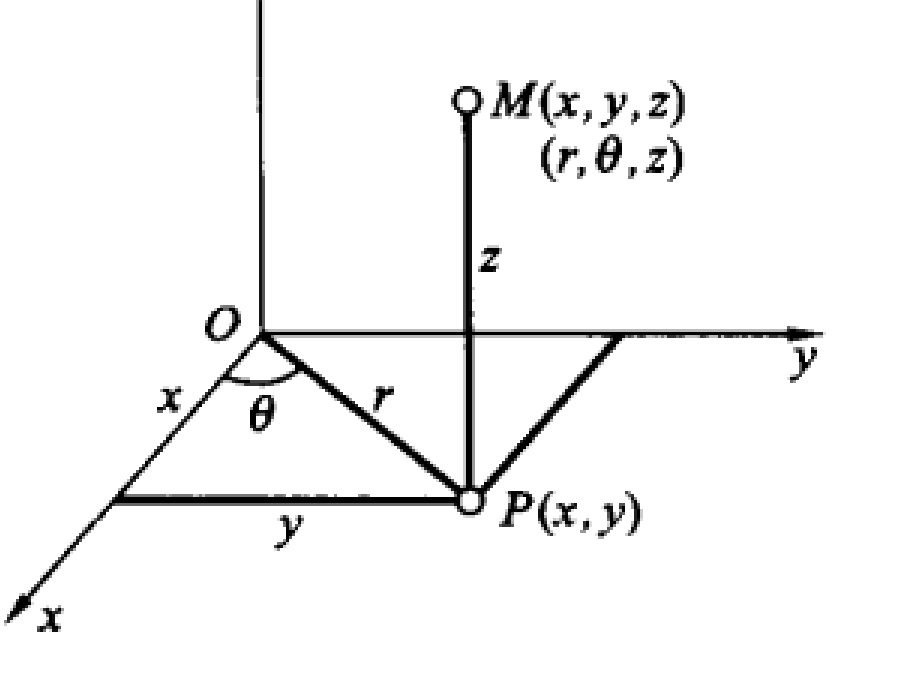
\includegraphics[width=0.32\textwidth]{work/figures/fig20-32}\caption{\relax}\label{fig:20-32}
\end{figure}

用柱坐标曲面网对 $V$ 作分法后，体积元的底面积近似于极坐标网下的面积元 $r\,\mathrm{d}r\,\mathrm{d}\theta$，而高为 $\mathrm{d}z$，因此在柱坐标下，体积元为 $r\,\mathrm{d}r\,\mathrm{d}\theta\,\mathrm{d}z$．这从图~\ref{fig:20-33} 看是显然的．

\begin{figure}[htbp]
\centering
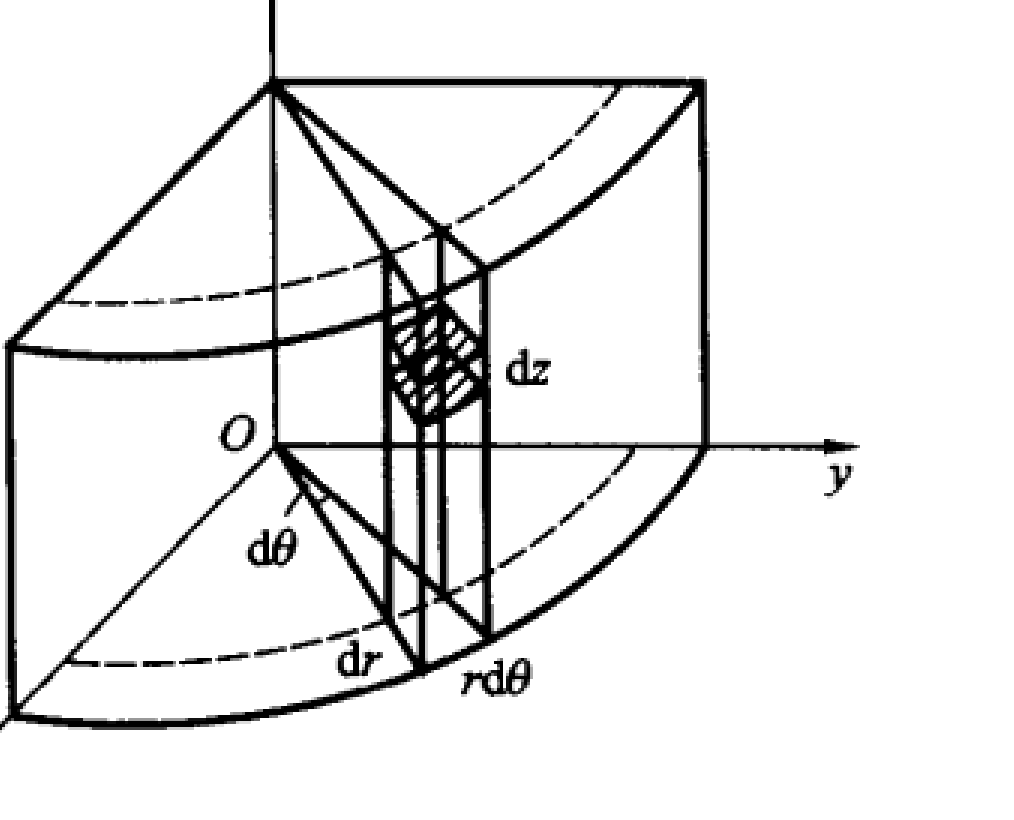
\includegraphics[width=0.36\textwidth]{work/figures/fig20-33}\caption{\relax}\label{fig:20-33}
\end{figure}

变量代换公式右边的积分通常化为累次积分来计算．将 $V$ 投影到 $Oxy$ 平面上，记该投影区域为 $D$，它的极坐标表示为 $\Delta$，则 $V$ 的柱坐标表示为
\[
\Omega=\left\{(r,\theta,z)\mid z_{1}(r,\theta)\leqslant z\leqslant z_{2}(r,\theta),(r,\theta)\in\Delta\right\}.
\]
因此
\[
\iiint_{V}f(x,y,z)\,\mathrm{d}x\mathrm{d}y\mathrm{d}z=\iint_{\Delta}r\,\mathrm{d}r\mathrm{d}\theta\int_{z_{1}(r,\theta)}^{z_{2}(r,\theta)}f(r\cos\theta,r\sin\theta,z)\,\mathrm{d}z.
\]

\begin{example}\label{ex:20-3-6}
求积分 $\displaystyle\iiint_{V}\frac{z}{\left(x^{2}+y^{2}+z^{2}\right)^{\frac{3}{2}}}\,\mathrm{d}x\mathrm{d}y\mathrm{d}z$．其中 $V$ 是柱面 $x^{2}+y^{2}=1$ 和锥面 $x^{2}+y^{2}=z^{2}$ $(z>0)$ 以及平面 $z=h$ $(h>1)$ 所围成的立体（见图~\ref{fig:20-34}）．
\end{example}

\begin{proof}[解]
作柱坐标变换
\[
x=r\cos\theta,\quad y=r\sin\theta,\quad z=z.
\]
则在柱坐标下，三曲面方程分别为 $r=1$，$r=z$，$z=h$，故 $V$ 在柱坐标下为
\[
\left\{(r,\theta,z)\mid r\leqslant z\leqslant h,0\leqslant r\leqslant 1,0\leqslant\theta\leqslant 2\pi\right\}.
\]

\begin{figure}[htbp]
\centering
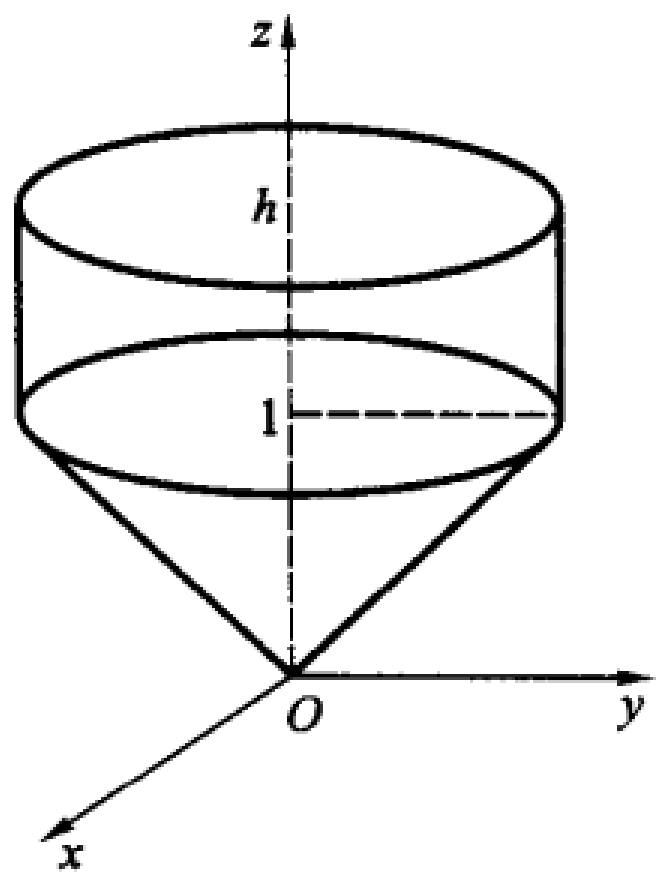
\includegraphics[width=0.28\textwidth]{work/figures/fig20-34}\caption{\relax}\label{fig:20-34}
\end{figure}

从而
\[
\begin{aligned}
&\iiint_{V}\frac{z}{\left(x^{2}+y^{2}+z^{2}\right)^{\frac{3}{2}}}\,\mathrm{d}x\mathrm{d}y\mathrm{d}z\\
=&\int_{0}^{2\pi}\mathrm{d}\theta\int_{0}^{1}r\,\mathrm{d}r\int_{r}^{h}\frac{z\,\mathrm{d}z}{\left(r^{2}+z^{2}\right)^{\frac{3}{2}}}\\
=&2\pi\int_{0}^{1}-r\left(r^{2}+z^{2}\right)^{-\frac{1}{2}}\bigg|_{r}^{h}\,\mathrm{d}r\\
=&2\pi\int_{0}^{1}r\left(\frac{1}{\sqrt{2}\,r}-\frac{1}{\sqrt{r^{2}+h^{2}}}\right)\mathrm{d}r\\
=&2\pi\left(\frac{r}{\sqrt{2}}-\sqrt{r^{2}+h^{2}}\right)\bigg|_{0}^{1}\\
=&2\pi\left(\frac{1}{\sqrt{2}}+h-\sqrt{1+h^{2}}\right).
\end{aligned}
\]
\end{proof}

（2）球坐标变换
\[
\begin{cases}
x=r\cos\theta\sin\varphi, & 0\leqslant r<+\infty,\\
y=r\sin\theta\sin\varphi, & 0\leqslant\theta<2\pi,\\
z=r\cos\varphi, & 0\leqslant\varphi\leqslant\pi.
\end{cases}
\]
这时
\[
\begin{aligned}
&J(r,\theta,\varphi)=\frac{\partial(x,y,z)}{\partial(r,\theta,\varphi)}\\
={}&\begin{vmatrix}
\cos\theta\sin\varphi & -r\sin\theta\sin\varphi & r\cos\theta\cos\varphi\\
\sin\theta\sin\varphi & r\cos\theta\sin\varphi & r\sin\theta\cos\varphi\\
\cos\varphi & 0 & -r\sin\varphi
\end{vmatrix}=-r^{2}\sin\varphi,
\end{aligned}
\]
因此变量代换公式为
\[
\begin{aligned}
&\iiint\limits_{V}f(x,y,z)\,\mathrm{d}x\mathrm{d}y\mathrm{d}z\\
=&\iiint\limits_{\Omega}f(r\cos\theta\sin\varphi,r\sin\theta\sin\varphi,r\cos\varphi)\,r^{2}\sin\varphi\,\mathrm{d}r\mathrm{d}\theta\mathrm{d}\varphi.
\end{aligned}
\]

下面从微元的观点来看看这个公式．在 $Oxyz$ 空间中，球坐标中的 $r$ 是点 $M(x,y,z)$ 到原点的距离，$\varphi$ 是矢径 $\overrightarrow{OM}$ 与 $z$ 轴正向的夹角，$\theta$ 则是矢径 $\overrightarrow{OM}$ 在 $Oxy$ 平面上的投影与 $x$ 轴正向的夹角（见图~\ref{fig:20-35}）．因此球坐标的三束坐标面组成的曲面网分别为：$r=$ 常数，它是以原点为球心的球面；$\theta=$ 常数，它是过 $z$ 轴的半平面；$\varphi=$ 常数则是以原点为顶点，以 $z$ 轴为中心轴的圆锥面．

\begin{figure}[htbp]
\centering
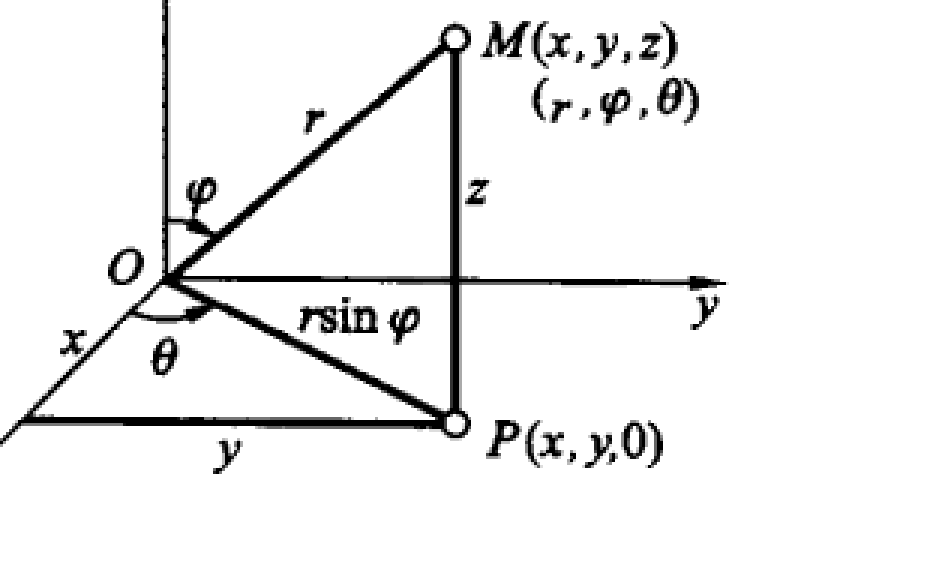
\includegraphics[width=0.34\textwidth]{work/figures/fig20-35}\caption{\relax}\label{fig:20-35}
\end{figure}

这时，体积元由半径为 $r$ 和 $r+\mathrm{d}r$ 的两块半球面，与 $Oxz$ 夹角为 $\theta$ 和 $\theta+\mathrm{d}\theta$ 的两块半平面以及与 $z$ 轴夹角为 $\varphi$ 和 $\varphi+\mathrm{d}\varphi$ 的两块锥面包围而成，其体积为（图~\ref{fig:20-36}）
\[
\mathrm{d}r\cdot r\mathrm{d}\varphi\cdot r\sin\varphi\mathrm{d}\theta=r^{2}\sin\varphi\,\mathrm{d}r\mathrm{d}\theta\mathrm{d}\varphi.
\]

\begin{figure}[htbp]
\centering
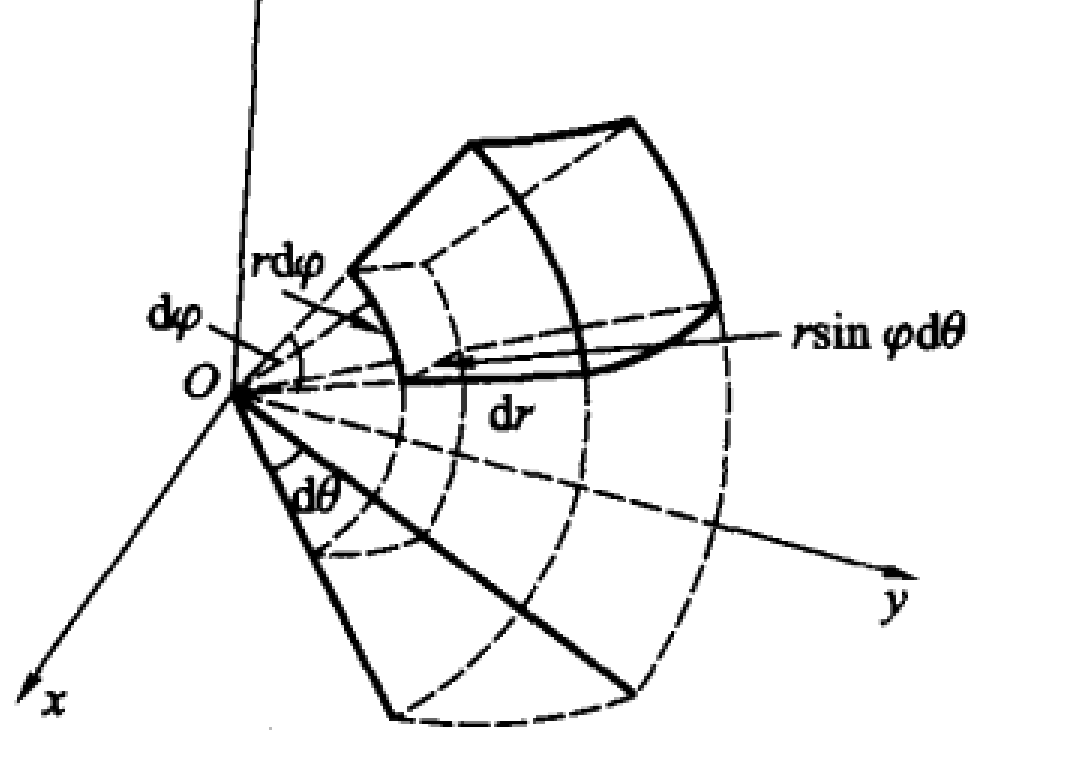
\includegraphics[width=0.38\textwidth]{work/figures/fig20-36}\caption{\relax}\label{fig:20-36}
\end{figure}

\begin{example}\label{ex:20-3-7}
求 $(x^{2}+y^{2}+z^{2})^{2}=az$ $(a>0)$ 所围区域（图~\ref{fig:20-37}）的体积．
\end{example}

\begin{proof}[解]
作球坐标变换
\[
x=r\cos\theta\sin\varphi,\quad y=r\sin\theta\sin\varphi,\quad z=r\cos\varphi.
\]
在球坐标下，曲面方程为 $r^{3}=a\cos\varphi$，区域 $V$ 可表为
\[
\left\{(r,\theta,\varphi)\mid 0\leqslant r\leqslant(a\cos\varphi)^{1/3},0\leqslant\varphi\leqslant\frac{\pi}{2},0\leqslant\theta\leqslant 2\pi\right\}.
\]

\begin{figure}[htbp]
\centering
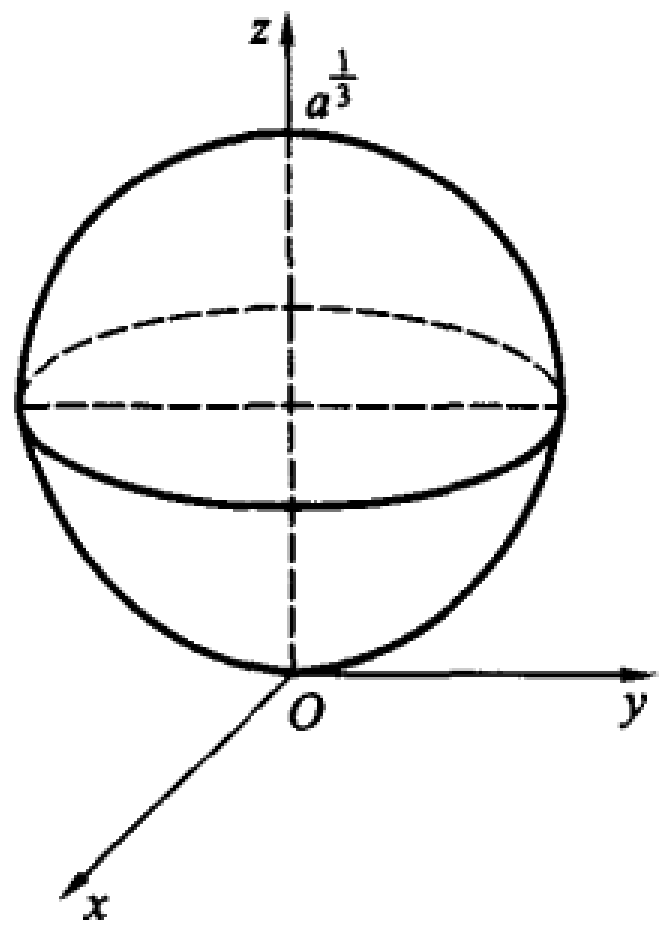
\includegraphics[width=0.28\textwidth]{work/figures/fig20-37}\caption{\relax}\label{fig:20-37}
\end{figure}

因此
\[
\begin{aligned}
V=&\iiint_{V}\mathrm{d}x\mathrm{d}y\mathrm{d}z=\int_{0}^{2\pi}\mathrm{d}\theta\int_{0}^{\frac{\pi}{2}}\mathrm{d}\varphi\int_{0}^{(a\cos\varphi)^{\frac{1}{3}}}r^{2}\sin\varphi\,\mathrm{d}r\\
=&2\pi\int_{0}^{\frac{\pi}{2}}\sin\varphi\cdot\frac{1}{3}r^{3}\bigg|_{0}^{(a\cos\varphi)^{\frac{1}{3}}}\,\mathrm{d}\varphi\\
=&\frac{2\pi a}{3}\int_{0}^{\frac{\pi}{2}}\sin\varphi\cos\varphi\,\mathrm{d}\varphi=\frac{1}{3}\pi a.
\end{aligned}
\]
\end{proof}

\begin{example}\label{ex:20-3-8}
求曲面
\[
\left(\frac{x^{2}}{a^{2}}+\frac{y^{2}}{b^{2}}+\frac{z^{2}}{c^{2}}\right)^{2}=ax\quad(a,b,c>0)
\]
所围区域的体积．
\end{example}

\begin{proof}[解]
作广义球坐标变换
\[
\begin{cases}
y=br\cos\theta\sin\varphi,\\
z=cr\sin\theta\sin\varphi,\\
x=ar\cos\varphi.
\end{cases}
\]
在变换下，曲面方程化为 $r^{3}=a^{2}\cos\varphi$．因此所围区域可表为
\[
\left\{(r,\theta,\varphi)\mid 0\leqslant\theta\leqslant 2\pi,0\leqslant\varphi\leqslant\frac{\pi}{2},0\leqslant r\leqslant(a^{2}\cos\varphi)^{\frac{1}{3}}\right\}.
\]
因为
\[
\frac{\partial(y,z,x)}{\partial(r,\theta,\varphi)}=-abcr^{2}\sin\varphi,
\]
所以
\[
V=\iiint_{V}\mathrm{d}x\mathrm{d}y\mathrm{d}z=\int_{0}^{2\pi}\mathrm{d}\theta\int_{0}^{\frac{\pi}{2}}\mathrm{d}\varphi\int_{0}^{(a^{2}\cos\varphi)^{\frac{1}{3}}}abcr^{2}\sin\varphi\,\mathrm{d}r,
\]
由上例结果便得
\[
V=\frac{1}{3}\pi a^{3}bc.
\]
\end{proof}

\begin{xiti}
\item 用极坐标变换将 $\displaystyle\iint_{D}f(x,y)\,\mathrm{d}x\,\mathrm{d}y$ 化为累次积分：
\begin{ziti}
\item $D$：半圆 $x^{2}+y^{2}\leqslant a^{2}$，$y\geqslant 0$；
\item $D$：半环 $a^{2}\leqslant x^{2}+y^{2}\leqslant b^{2}$，$x\geqslant 0$；
\item $D$：圆 $x^{2}+y^{2}\leqslant ay$ $(a>0)$；
\item $D$：正方形 $0\leqslant x\leqslant a$，$0\leqslant y\leqslant a$．
\end{ziti}
\item 用极坐标变换计算下列二重积分：
\begin{ziti}
\item $\displaystyle\iint_{D}\sin\sqrt{x^{2}+y^{2}}\,\mathrm{d}x\,\mathrm{d}y$，$D$：$\pi^{2}\leqslant x^{2}+y^{2}\leqslant 4\pi^{2}$；
\item $\displaystyle\iint_{D}(x+y)\,\mathrm{d}x\,\mathrm{d}y$，$D$ 是圆 $x^{2}+y^{2}\leqslant x+y$ 的内部；
\item $\displaystyle\iint_{D}(x^{2}+y^{2})\,\mathrm{d}x\mathrm{d}y$，$D$ 由双纽线 $(x^{2}+y^{2})^{2}=a^{2}(x^{2}-y^{2})$ $(x\geqslant 0)$ 围成；
\item $\displaystyle\iint_{D}x\,\mathrm{d}x\,\mathrm{d}y$，$D$ 由阿基米德螺线 $r=\theta$ 在 $\theta\in[0,\pi]$ 的一段和半射线 $\theta=\pi$ 围成；
\item $\displaystyle\iint_{D}xy\,\mathrm{d}x\,\mathrm{d}y$，$D$ 由对数螺线 $r=\mathrm{e}^{\theta}$ 在 $\theta\in\left[0,\dfrac{\pi}{2}\right]$ 的一段和半射线 $\theta=0$，$\theta=\dfrac{\pi}{2}$ 围成．
\end{ziti}
\item 在下列积分中引入新变量 $u$，$v$，将它们化为累次积分：
\begin{ziti}
\item $\displaystyle\int_{0}^{2}\mathrm{d}x\int_{1-x}^{2-x}f(x,y)\,\mathrm{d}y$，若 $u=x+y$，$v=x-y$；
\item $\displaystyle\int_{a}^{b}\mathrm{d}x\int_{\alpha x}^{\beta x}f(x,y)\,\mathrm{d}y$ $\left(0<a<b,0<\alpha<\beta\right)$，若 $u=x$，$v=\dfrac{y}{x}$；
\item $\displaystyle\iint_{D}f(x,y)\,\mathrm{d}x\mathrm{d}y$，其中 $D=\left\{(x,y)\mid\sqrt{x}+\sqrt{y}\leqslant\sqrt{a},x\geqslant 0,y\geqslant 0\right\}$，若 $x=u\cos^{4}v$，$y=u\sin^{4}v$；
\item $\displaystyle\iint_{D}f(x,y)\,\mathrm{d}x\mathrm{d}y$，其中 $D=\left\{(x,y)\mid x+y\leqslant a,x\geqslant 0,y\geqslant 0\right\}$ $(a>0)$，若 $x+y=u$，$y=uv$．
\end{ziti}
\item 作适当的变量代换，求下列积分：
\begin{ziti}
\item $\displaystyle\iint_{D}(x^{2}+y^{2})\,\mathrm{d}x\mathrm{d}y$，$D$ 是由 $x^{4}+y^{4}=1$ 围成的区域；
\item $\displaystyle\iint_{D}(x+y)\,\mathrm{d}x\,\mathrm{d}y$，$D$ 由 $y=4x^{2}$，$y=9x^{2}$，$x=4y^{2}$，$x=9y^{2}$ 围成；
\item $\displaystyle\iint_{D}xy\,\mathrm{d}x\,\mathrm{d}y$，$D$ 由 $xy=2$，$xy=4$，$y=x$，$y=2x$ 围成．
\end{ziti}
\item 利用二重积分求由下列曲面围成的立体的体积：
\begin{ziti}
\item $z=xy$，$x^{2}+y^{2}=a^{2}$，$z=0$；
\item $z=\dfrac{h}{R}\sqrt{x^{2}+y^{2}}$，$z=0$，$x^{2}+y^{2}=R^{2}$；
\item 球面 $x^{2}+y^{2}+z^{2}=a^{2}$ 与圆柱面 $x^{2}+y^{2}=ax$ $(a>0)$ 的公共部分；
\item $\dfrac{x^{2}}{a^{2}}+\dfrac{y^{2}}{b^{2}}+\dfrac{z^{2}}{c^{2}}=1$，$\dfrac{x^{2}}{a^{2}}+\dfrac{y^{2}}{b^{2}}=\dfrac{z^{2}}{c^{2}}$ $(z>0)$；
\item $z^{2}=\dfrac{x^{2}}{4}+\dfrac{y^{2}}{9}$，$2z=\dfrac{x^{2}}{4}+\dfrac{y^{2}}{9}$；
\item $z=x^{2}+y^{2}$，$z=x+y$．
\end{ziti}
\item 求曲线 $\left(\dfrac{x^{2}}{a^{2}}+\dfrac{y^{2}}{b^{2}}\right)^{2}=\dfrac{xy}{c^{2}}$ 所围的面积．
\item 用柱坐标变换计算下列三重积分：
\begin{ziti}
\item $\displaystyle\iiint_{V}(x^{2}+y^{2})^{2}\,\mathrm{d}x\mathrm{d}y\mathrm{d}z$，$V$ 由曲面 $z=x^{2}+y^{2}$，$z=4$，$z=16$ 围成；
\item $\displaystyle\iiint\limits_{V}\left(\sqrt{x^{2}+y^{2}}\right)^{3}\,\mathrm{d}x\mathrm{d}y\mathrm{d}z$，$V$ 由曲面 $x^{2}+y^{2}=9$，$x^{2}+y^{2}=16$，$z^{2}=x^{2}+y^{2}$，$z\geqslant 0$ 围成．
\end{ziti}
\item 用球坐标变换计算下列三重积分：
\begin{ziti}
\item $\displaystyle\iiint_{V}(x+y+z)\,\mathrm{d}x\,\mathrm{d}y\,\mathrm{d}z$，$V$：$x^{2}+y^{2}+z^{2}\leqslant R^{2}$；
\item $\displaystyle\iiint_{V}\left(\sqrt{x^{2}+y^{2}+z^{2}}\right)^{5}\,\mathrm{d}x\mathrm{d}y\mathrm{d}z$，$V$ 由 $x^{2}+y^{2}+z^{2}=2z$ 围成；
\item $\displaystyle\iiint_{V}x^{2}\,\mathrm{d}x\,\mathrm{d}y\,\mathrm{d}z$，$V$ 是 $x^{2}+y^{2}\leqslant z^{2}$，$x^{2}+y^{2}+z^{2}\leqslant 8$ 的公共部分．
\end{ziti}
\item 作适当的变量代换，求下列三重积分：
\begin{ziti}
\item $\displaystyle\iiint_{V}x^{2}y^{2}z\,\mathrm{d}x\,\mathrm{d}y\,\mathrm{d}z$，$V$ 由 $z=\dfrac{x^{2}+y^{2}}{a}$，$z=\dfrac{x^{2}+y^{2}}{b}$，$xy=c$，$xy=d$，$y=\alpha x$，$y=\beta x$ 围成的立体，其中 $0<a<b$，$0<c<d$，$0<\alpha<\beta$；
\item $\displaystyle\iiint_{V}x^{2}yz\,\mathrm{d}x\mathrm{d}y\mathrm{d}z$，$V$ 同（1）；
\item $\displaystyle\iiint_{V}y^{4}\,\mathrm{d}x\,\mathrm{d}y\,\mathrm{d}z$，$V$ 由 $x=az^{2}$，$x=bz^{2}$ $(z>0,0<a<b)$，$x=\alpha y$，$x=\beta y$ $(0<\alpha<\beta)$ 以及 $x=h$ $(>0)$ 围成；
\item $\displaystyle\iiint_{V}\mathrm{e}^{\sqrt{\frac{x^{2}}{a^{2}}+\frac{y^{2}}{b^{2}}+\frac{z^{2}}{c^{2}}}}\,\mathrm{d}x\mathrm{d}y\mathrm{d}z$，$V$ 由 $\dfrac{x^{2}}{a^{2}}+\dfrac{y^{2}}{b^{2}}+\dfrac{z^{2}}{c^{2}}=1$ 围成；
\item $\displaystyle\int_{0}^{1}\mathrm{d}x\int_{0}^{\sqrt{1-x^{2}}}\mathrm{d}y\int_{\sqrt{x^{2}+y^{2}}}^{\sqrt{2-x^{2}-y^{2}}}z^{2}\,\mathrm{d}z$．
\end{ziti}
\item 求下列各曲面所围立体之体积：
\begin{ziti}
\item $z=x^{2}+y^{2}$，$z=2(x^{2}+y^{2})$，$y=x$，$y=x^{2}$；
\item $\left(\dfrac{x}{a}+\dfrac{y}{b}\right)^{2}+\left(\dfrac{z}{c}\right)^{2}=1$ $\quad(x\geqslant 0,y\geqslant 0,z\geqslant 0,a>0,b>0,c>0)$．
\end{ziti}
\end{xiti}

\section{曲面面积}\label{sec:20-4}

作为二重积分的应用，本节讲述一般空间曲面面积的求法．首先碰到的问题是，什么叫空间曲面的面积？

回忆曲线的情形，在第八章 §2 中，我们曾把平面曲线的长度定义为内接折线长的极限，并把它用定积分表示出来．定义曲面面积的一种自然想法，就是模仿这个思路进行．

对于平面曲线，可以用内接折线来近似弧长，那么对空间曲面，能否用内接多面形来近似曲面面积呢？如果在曲面上任取四点，它们未必在同一平面上，因此一般不存在用平面四边形作成内接多面形．如果在曲面上任取三点，虽然三点可确定一平面，即可有平面三角形作成内接多面形，但当三角形的最大边长趋于零时，内接多面形的面积之和未必有确定的极限，即使有极限也未必与我们直观了解的面积相同．施瓦茨就曾证明：对圆柱面来说，这种内接三角形面积和的极限，依赖于三角形的高与底的比例，因而极限是不存在的（图~\ref{fig:20-38}）．因此，如果这样来定义曲面面积，则圆柱面也没有面积，这显然与常识不符．究其原因，就在于曲面的法向量与它的内接三角形的法向量可以任意地接近于垂直，即使三角形的最大边长任意小．因此这样的多面体的面积不可能作为曲面面积的近似值．

\begin{figure}[htbp]
\centering
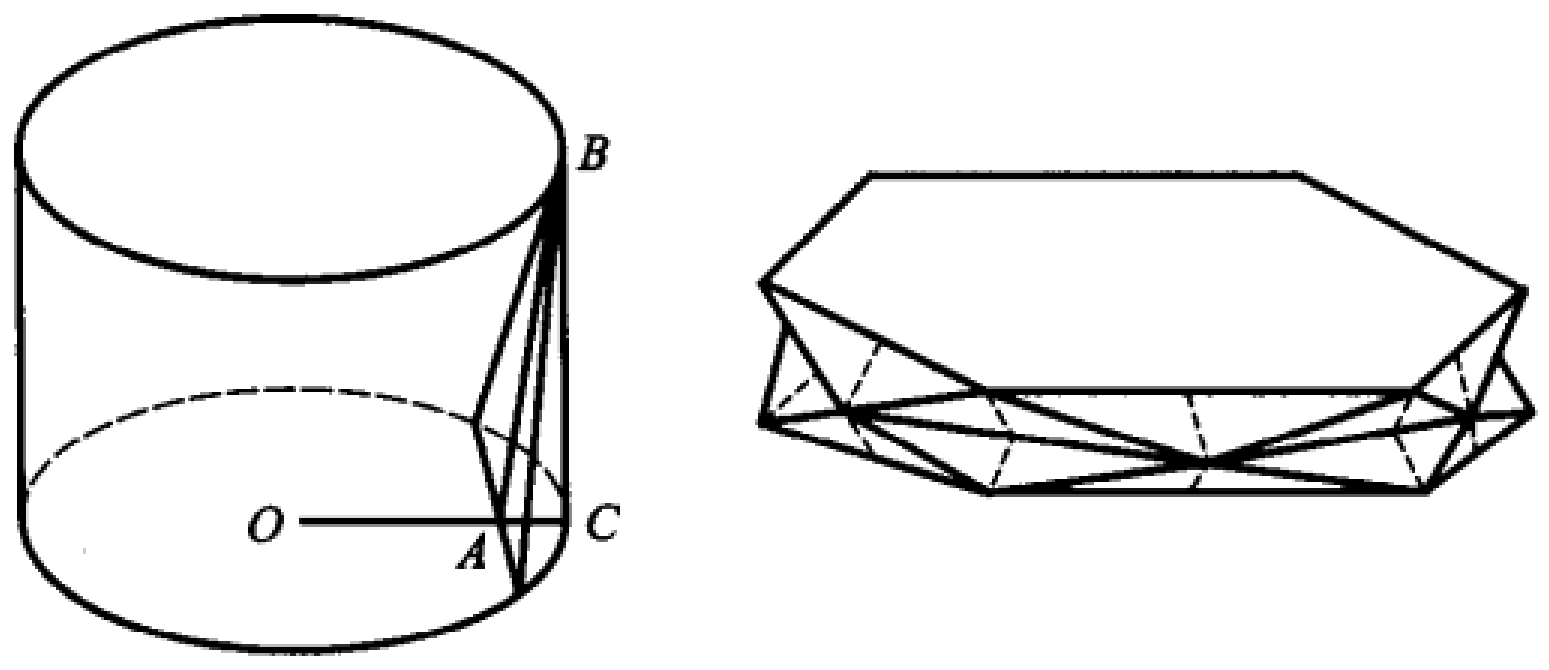
\includegraphics[width=0.55\textwidth]{work/figures/fig20-38}\caption{\relax}\label{fig:20-38}
\end{figure}

这个原因也启发我们考虑用切平面的小块面积近似小块曲面的面积，这时可以保证曲面与近似它的平面的方向保持一致．其实，在局部，曲线的弧长也是可以用切线近似的，这可以从微分三角形看出（图~\ref{fig:20-39}）：
\[
\mathrm{d}s^{2}=\mathrm{d}x^{2}+\mathrm{d}y^{2}.
\]

\begin{figure}[htbp]
\centering
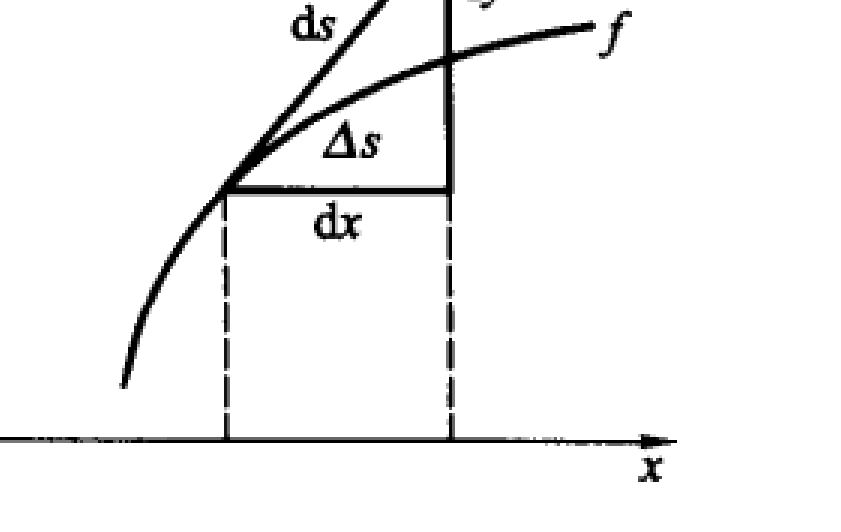
\includegraphics[width=0.32\textwidth]{work/figures/fig20-39}\caption{\relax}\label{fig:20-39}
\end{figure}

下面我们用这个办法来定义曲面的面积．先考虑曲面 $S$ 由函数
\[
z=f(x,y),\quad(x,y)\in D
\]
给出，其中 $D$ 是由逐段光滑的曲线围成．若 $f$ 具有对 $x$，$y$ 的连续偏导数，则称这曲面是\emph{光滑}的．这时曲面上任一点都存在切平面．

任意给 $D$ 一个分法 $\Delta D_{i}$ $(i=1,2,\cdots,n)$．对应于这个分法，曲面被分为 $n$ 小块 $\Delta S_{i}$，使得 $\Delta S_{i}$ 在 $Oxy$ 平面上的投影恰为 $\Delta D_{i}$．任取 $(\xi_{i},\eta_{i})\in\Delta D_{i}$，记 $\zeta_{i}=f(\xi_{i},\eta_{i})$，在曲面上的点 $(\xi_{i},\eta_{i},\zeta_{i})$ 处作切平面，并记切平面上与 $\Delta S_{i}$ 有公共投影 $\Delta D_{i}$ 的一小块为 $\Delta\sigma_{i}$，它的面积应是小块曲面 $\Delta S_{i}$ 面积（如果存在的话）的近似．记 $\lambda=\max\limits_{1\leqslant i\leqslant n}\left\{d(\Delta D_{i})\right\}$，其中 $d(\Delta D_{i})$ 是 $\Delta D_{i}$ 的直径．如果当 $\lambda\to 0$ 时，$\sum\limits_{i=1}^{n}\Delta\sigma_{i}$ 的极限存在，则称曲面 $S$ 是有面积的，且这极限便是曲面的面积：
\[
S=\lim_{\lambda\to 0}\sum_{i=1}^{n}\Delta\sigma_{i}.
\]

下面我们来计算 $\Delta\sigma_{i}$．若 $\Delta\sigma_{i}$ 的法向量 $\bm{n}_{i}$ 的方向余弦为
\[
\left(\cos\alpha_{i},\cos\beta_{i},\cos\gamma_{i}\right),
\]
则显然
\[
\Delta\sigma_{i}=\frac{\Delta D_{i}}{\left|\cos\gamma_{i}\right|}.
\]
回忆光滑曲面 $z=f(x,y)$ 在 $(\xi_{i},\eta_{i},\zeta_{i})$ 点的法向量的求法，知
\[
\bm{n}_{i}=\pm\left(f_{x}(\xi_{i},\eta_{i}),f_{y}(\xi_{i},\eta_{i}),-1\right),
\]
它与 $z$ 轴的夹角余弦为
\[
\cos\gamma_{i}=\frac{\pm 1}{\sqrt{1+f_{x}^{2}(\xi_{i},\eta_{i})+f_{y}^{2}(\xi_{i},\eta_{i})}},
\]
因此
\[
\sum_{i=1}^{n}\Delta\sigma_{i}=\sum_{i=1}^{n}\frac{\Delta D_{i}}{\left|\cos\gamma_{i}\right|}=\sum_{i=1}^{n}\sqrt{1+f_{x}^{2}(\xi_{i},\eta_{i})+f_{y}^{2}(\xi_{i},\eta_{i})}\,\Delta D_{i},
\]
上式右端恰是函数 $F(x,y)=\sqrt{1+f_{x}^{2}(x,y)+f_{y}^{2}(x,y)}$ 的黎曼和．而 $f_{x}$ 和 $f_{y}$ 在 $D$ 上连续，故 $F(x,y)$ 在 $D$ 连续．从而可积．即存在极限
\[
\begin{aligned}
S&=\lim_{\lambda\to 0}\sum_{i=1}^{n}\sqrt{1+f_{x}^{2}(\xi_{i},\eta_{i})+f_{y}^{2}(\xi_{i},\eta_{i})}\,\Delta D_{i}\\
&=\iint_{D}\sqrt{1+f_{x}^{2}(x,y)+f_{y}^{2}(x,y)}\,\mathrm{d}x\mathrm{d}y.
\end{aligned}
\]
这就是曲面 $S$ 的面积计算公式，它是 $D$ 上的一个二重积分．记
\[
\mathrm{d}S=\sqrt{1+f_{x}^{2}(x,y)+f_{y}^{2}(x,y)}\,\mathrm{d}x\mathrm{d}y=\frac{\mathrm{d}x\mathrm{d}y}{\left|\cos\gamma\right|},
\]
并称之为曲面的\emph{面积元}，它的几何意义是：曲面的面积元 $\mathrm{d}S$ 在 $Oxy$ 平面上的投影就是 $Oxy$ 平面上的面积元 $\mathrm{d}x\,\mathrm{d}y$．

\begin{example}\label{ex:20-4-1}
计算 $x^{2}+y^{2}+z^{2}=R^{2}$ 被 $x^{2}+y^{2}\leqslant Rx$ 所截出的曲面的面积．
\end{example}

\begin{proof}[解]
曲面的图形如图~\ref{fig:20-40}．由对称性，只要求出位于上半球面的那一部分，再乘 $2$ 即可．球面方程 $x^{2}+y^{2}+z^{2}=R^{2}$ 对 $x$ 求导得

\begin{figure}[htbp]
\centering
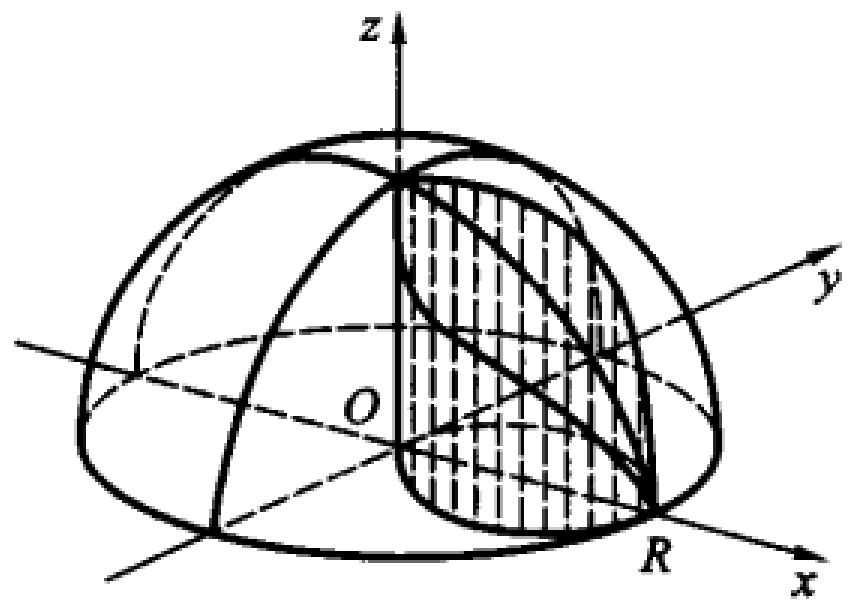
\includegraphics[width=0.34\textwidth]{work/figures/fig20-40}\caption{\relax}\label{fig:20-40}
\end{figure}
\[
2x+2z\frac{\partial z}{\partial x}=0,
\]
因此 $\dfrac{\partial z}{\partial x}=-\dfrac{x}{z}$．同理可得 $\dfrac{\partial z}{\partial y}=-\dfrac{y}{z}$．故在球面上有
\[
\begin{aligned}
&\sqrt{1+\left(\frac{\partial z}{\partial x}\right)^{2}+\left(\frac{\partial z}{\partial y}\right)^{2}}\\
=&\sqrt{1+\left(\frac{x}{z}\right)^{2}+\left(\frac{y}{z}\right)^{2}}=\frac{\sqrt{x^{2}+y^{2}+z^{2}}}{z}=\frac{R}{\sqrt{R^{2}-x^{2}-y^{2}}}.
\end{aligned}
\]
于是所求面积为
\[
S=2\iint_{D}\frac{R}{\sqrt{R^{2}-x^{2}-y^{2}}}\,\mathrm{d}x\mathrm{d}y,
\]
其中 $D$ 为 $x^{2}+y^{2}\leqslant Rx$．作极坐标变换
\[
x=r\cos\theta,\quad y=r\sin\theta,
\]
得
\[
\begin{aligned}
S&=2\iint_{D}\frac{R}{\sqrt{R^{2}-x^{2}-y^{2}}}\,\mathrm{d}x\mathrm{d}y\\
&=2R\int_{-\frac{\pi}{2}}^{\frac{\pi}{2}}\mathrm{d}\theta\int_{0}^{R\cos\theta}\frac{r\,\mathrm{d}r}{\sqrt{R^{2}-r^{2}}}\\
&=2R\int_{-\frac{\pi}{2}}^{\frac{\pi}{2}}\sqrt{R^{2}-r^{2}}\Bigg|_{R\cos\theta}^{0}\,\mathrm{d}\theta\\
&=2R\int_{-\frac{\pi}{2}}^{\frac{\pi}{2}}\left[R-R\left|\sin\theta\right|\right]\mathrm{d}\theta\\
&=4R^{2}\int_{0}^{\frac{\pi}{2}}(1-\sin\theta)\,\mathrm{d}\theta=4R^{2}\left(\frac{\pi}{2}-1\right).
\end{aligned}
\]
\end{proof}

\begin{figure}[htbp]
\centering
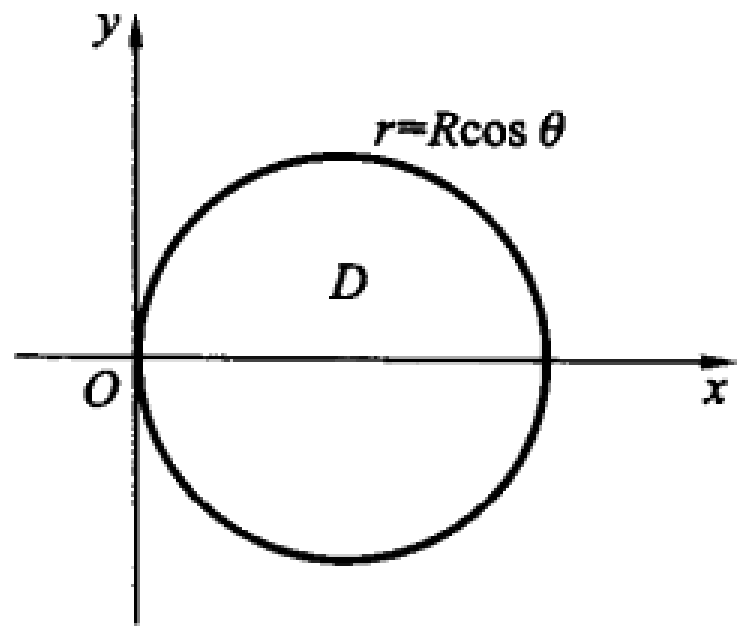
\includegraphics[width=0.34\textwidth]{work/figures/fig20-41}\caption{\relax}\label{fig:20-41}
\end{figure}

如果曲面由参数方程
\[
x=x(u,v),\quad y=y(u,v),\quad z=z(u,v),\quad(u,v)\in D
\]
给出，设函数 $x(u,v)$，$y(u,v)$，$z(u,v)$ 在 $D$ 上具有连续的一阶偏导数，且
\[
\begin{pmatrix}
\dfrac{\partial x}{\partial u} & \dfrac{\partial y}{\partial u} & \dfrac{\partial z}{\partial u}\\[6pt]
\dfrac{\partial x}{\partial v} & \dfrac{\partial y}{\partial v} & \dfrac{\partial z}{\partial v}
\end{pmatrix}
\]
在 $D$ 每一点的秩均为 $2$，则曲面是光滑曲面．曲面上每一点的法向量为
\[
\begin{aligned}
\bm{n}&=\pm\left(\frac{\partial(y,z)}{\partial(u,v)},\frac{\partial(z,x)}{\partial(u,v)},\frac{\partial(x,y)}{\partial(u,v)}\right)\\
&=\pm\begin{vmatrix}
\bm{i} & \bm{j} & \bm{k}\\
\dfrac{\partial x}{\partial u} & \dfrac{\partial y}{\partial u} & \dfrac{\partial z}{\partial u}\\[6pt]
\dfrac{\partial x}{\partial v} & \dfrac{\partial y}{\partial v} & \dfrac{\partial z}{\partial v}
\end{vmatrix}=\pm\left(\bm{r}_{u}\times\bm{r}_{v}\right),
\end{aligned}
\]
其中 $\bm{r}_{u}=\left(\dfrac{\partial x}{\partial u},\dfrac{\partial y}{\partial u},\dfrac{\partial z}{\partial u}\right)$，$\bm{r}_{v}=\left(\dfrac{\partial x}{\partial v},\dfrac{\partial y}{\partial v},\dfrac{\partial z}{\partial v}\right)$，并且 $\bm{n}$ 的三个分量中至少有一个分量不为零，为方便，记
\[
A=\frac{\partial(y,z)}{\partial(u,v)},\quad B=\frac{\partial(z,x)}{\partial(u,v)},\quad C=\frac{\partial(x,y)}{\partial(u,v)}.
\]
这样，$\bm{n}=\pm(A,B,C)$．不妨设 $C\neq 0$，这时
\[
\cos(\bm{n},z)=\frac{\pm C}{\sqrt{A^{2}+B^{2}+C^{2}}},
\]
由二重积分的变量代换公式，有
\[
\begin{aligned}
S&=\iint_{D'}\frac{\mathrm{d}x\mathrm{d}y}{\left|\cos(\bm{n},z)\right|}=\iint_{D}\frac{\left|C\right|}{\left|\cos(\bm{n},z)\right|}\,\mathrm{d}u\mathrm{d}v\\
&=\iint_{D}\sqrt{A^{2}+B^{2}+C^{2}}\,\mathrm{d}u\mathrm{d}v.
\end{aligned}
\]
由于在参数形式下，$x$，$y$，$z$ 处于同等地位，不论 $\bm{n}$ 的哪个分量不为零都可以得到同样的积分表达式
\[
S=\iint\limits_{D}\sqrt{A^{2}+B^{2}+C^{2}}\,\mathrm{d}u\mathrm{d}v,
\]
这就是在参数形式下曲面的面积公式．为便于计算，可以将积分表达式进一步变形．注意到
\[
\begin{aligned}
A^{2}+B^{2}+C^{2}&=\bm{n}\cdot\bm{n}=\left|\bm{n}\right|^{2}=\left|\bm{r}_{u}\times\bm{r}_{v}\right|^{2}\\
&=\left|\bm{r}_{u}\right|^{2}\left|\bm{r}_{v}\right|^{2}\sin^{2}(\bm{r}_{u},\bm{r}_{v})\\
&=\left|\bm{r}_{u}\right|^{2}\left|\bm{r}_{v}\right|^{2}\left(1-\cos^{2}(\bm{r}_{u},\bm{r}_{v})\right)\\
&=\left|\bm{r}_{u}\right|^{2}\left|\bm{r}_{v}\right|^{2}\left[1-\left(\frac{\bm{r}_{u}\cdot\bm{r}_{v}}{\left|\bm{r}_{u}\right|\cdot\left|\bm{r}_{v}\right|}\right)^{2}\right]\\
&=\left|\bm{r}_{u}\right|^{2}\left|\bm{r}_{v}\right|^{2}-\left(\bm{r}_{u}\cdot\bm{r}_{v}\right)^{2}.
\end{aligned}
\]
记
\[
\begin{aligned}
E&=\left|\bm{r}_{u}\right|^{2}=\left(\frac{\partial x}{\partial u}\right)^{2}+\left(\frac{\partial y}{\partial u}\right)^{2}+\left(\frac{\partial z}{\partial u}\right)^{2},\\
G&=\left|\bm{r}_{v}\right|^{2}=\left(\frac{\partial x}{\partial v}\right)^{2}+\left(\frac{\partial y}{\partial v}\right)^{2}+\left(\frac{\partial z}{\partial v}\right)^{2},\\
F&=\left(\bm{r}_{u}\cdot\bm{r}_{v}\right)=\frac{\partial x}{\partial u}\frac{\partial x}{\partial v}+\frac{\partial y}{\partial u}\frac{\partial y}{\partial v}+\frac{\partial z}{\partial u}\frac{\partial z}{\partial v}.
\end{aligned}
\]
则曲面的面积又可表为
\[
S=\iint_{D}\sqrt{EG-F^{2}}\,\mathrm{d}u\mathrm{d}v,
\]
这种形式既便于记忆，又便于计算．

\begin{example}\label{ex:20-4-2}
用参数形式求解例~\ref{ex:20-4-1}．
\end{example}

\begin{proof}[解]
球面 $x^{2}+y^{2}+z^{2}=R^{2}$ 的参数表示为
\[
\begin{aligned}
&x=R\cos\theta\sin\varphi,\quad y=R\sin\theta\sin\varphi,\quad z=R\cos\varphi,\\
&0\leqslant\theta\leqslant 2\pi,\ 0\leqslant\varphi\leqslant\pi.
\end{aligned}
\]
代入 $x^{2}+y^{2}\leqslant Rx$ 得
\[
\sin\varphi\leqslant\cos\theta,\quad-\frac{\pi}{2}\leqslant\theta\leqslant\frac{\pi}{2}.
\]
考虑第一卦限，则问题化为求球面位于
\[
D\colon 0\leqslant\varphi\leqslant\arcsin\cos\theta,\ 0\leqslant\theta\leqslant\frac{\pi}{2}
\]
部分的面积，然后再取 $4$ 倍即可．写出
\[
\begin{pmatrix}
\dfrac{\partial x}{\partial\theta} & \dfrac{\partial y}{\partial\theta} & \dfrac{\partial z}{\partial\theta}\\[6pt]
\dfrac{\partial x}{\partial\varphi} & \dfrac{\partial y}{\partial\varphi} & \dfrac{\partial z}{\partial\varphi}
\end{pmatrix}=\begin{pmatrix}
-R\sin\theta\sin\varphi & R\cos\theta\sin\varphi & 0\\
R\cos\theta\cos\varphi & R\sin\theta\cos\varphi & -R\sin\varphi
\end{pmatrix},
\]
\[
\begin{aligned}
E&=\left(R\sin\theta\sin\varphi\right)^{2}+\left(R\cos\theta\sin\varphi\right)^{2}=R^{2}\sin^{2}\varphi,\\
G&=\left(R\cos\theta\cos\varphi\right)^{2}+\left(R\sin\theta\cos\varphi\right)^{2}+\left(R\sin\varphi\right)^{2}=R^{2},\\
F&=0.
\end{aligned}
\]
故面积
\[
\begin{aligned}
S&=4\iint\limits_{D}\sqrt{EG-F^{2}}\,\mathrm{d}\theta\mathrm{d}\varphi\\
&=4\int_{0}^{\frac{\pi}{2}}\mathrm{d}\theta\int_{0}^{\arcsin\cos\theta}R^{2}\sin\varphi\,\mathrm{d}\varphi\\
&=4R^{2}\int_{0}^{\frac{\pi}{2}}(1-\sin\theta)\,\mathrm{d}\theta=4R^{2}\left(\frac{\pi}{2}-1\right),
\end{aligned}
\]
和前面计算的结果一样．
\end{proof}

\begin{xiti}
\item 求下列曲面的面积：
\begin{ziti}
\item $z=axy$ 包含在圆柱 $x^{2}+y^{2}=a^{2}$ 内的部分；
\item 锥面 $x^{2}+y^{2}=\dfrac{1}{3}z^{2}$ 与平面 $x+y+z=2a$ $(a>0)$ 所界部分的表面；
\item 锥面 $z=\sqrt{x^{2}+y^{2}}$ 被柱面 $z^{2}=2x$ 所截部分；
\item 曲面 $z=\sqrt{2xy}$ 被平面 $x+y=1$，$x=1$ 及 $y=1$ 所截下的部分．
\end{ziti}
\item 求螺旋面 $x=r\cos\varphi$，$y=r\sin\varphi$，$z=h\varphi$ $(0<r<a,\ 0<\varphi<2\pi)$ 的面积．
\item 求环面 $x=(b+a\cos\psi)\cos\varphi$，$y=(b+a\cos\psi)\sin\varphi$，$z=a\sin\psi$ $(0<a\leqslant b)$ 被两条经线 $\varphi=\varphi_{1}$，$\varphi=\varphi_{2}$ 和两条纬线 $\psi=\psi_{1}$，$\psi=\psi_{2}$ 所围成部分的面积，并求出整个环面的面积．
\end{xiti}

\section{重积分的物理应用}\label{sec:20-5}

\subsection{质心}

设 $\Omega$ 是空间的一块物体，$\rho(P)$ 是 $\Omega$ 的密度函数，它在 $\Omega$ 上连续．将 $\Omega$ 分为 $n$ 小块 $\Delta\Omega_{i}$ $(i=1,2,\cdots,n)$．由 $\rho(P)$ 的连续性，当 $\lambda=\max\limits_{1\leqslant i\leqslant n}\left\{\Delta\Omega_{i}\ \text{的直径}\right\}$ 充分小时，$\Delta\Omega_{i}$ 的质量 $\Delta m_{i}$ 有近似式
\[
\Delta m_{i}\approx\rho(P_{i})\Delta\Omega_{i},
\]
其中 $P_{i}$ 是 $\Delta\Omega_{i}$ 上的任一点．这时 $\Omega$ 可近似地视为 $n$ 个质量为 $\Delta m_{i}$ 的质点构成的质点系，质点分别位于点 $P_{i}(x_{i},y_{i},z_{i})$．因此质点系的质心坐标为
\[
\begin{aligned}
\bar{x}_{n}&=\frac{\displaystyle\sum_{i=1}^{n}x_{i}\rho(P_{i})\Delta\Omega_{i}}{\displaystyle\sum_{i=1}^{n}\rho(P_{i})\Delta\Omega_{i}},\\
\bar{y}_{n}&=\frac{\displaystyle\sum_{i=1}^{n}y_{i}\rho(P_{i})\Delta\Omega_{i}}{\displaystyle\sum_{i=1}^{n}\rho(P_{i})\Delta\Omega_{i}},\\
\bar{z}_{n}&=\frac{\displaystyle\sum_{i=1}^{n}z_{i}\rho(P_{i})\Delta\Omega_{i}}{\displaystyle\sum_{i=1}^{n}\rho(P_{i})\Delta\Omega_{i}},
\end{aligned}
\]
令 $\lambda\to 0$，由连续函数的可积性即得
\[
\begin{aligned}
\bar{x}&=\frac{\displaystyle\int_{\Omega}x\,\rho(P)\,\mathrm{d}\Omega}{\displaystyle\int_{\Omega}\rho(P)\,\mathrm{d}\Omega}=\frac{\displaystyle\int_{\Omega}x\,\mathrm{d}m}{\displaystyle\int_{\Omega}\mathrm{d}m},\\
\bar{y}&=\frac{\displaystyle\int_{\Omega}y\,\rho(P)\,\mathrm{d}\Omega}{\displaystyle\int_{\Omega}\rho(P)\,\mathrm{d}\Omega}=\frac{\displaystyle\int_{\Omega}y\,\mathrm{d}m}{\displaystyle\int_{\Omega}\mathrm{d}m},\\
\bar{z}&=\frac{\displaystyle\int_{\Omega}z\,\rho(P)\,\mathrm{d}\Omega}{\displaystyle\int_{\Omega}\rho(P)\,\mathrm{d}\Omega}=\frac{\displaystyle\int_{\Omega}z\,\mathrm{d}m}{\displaystyle\int_{\Omega}\mathrm{d}m}.
\end{aligned}
\]
这就是 $\Omega$ 的质心坐标公式，其中 $\mathrm{d}m=\rho(P)\mathrm{d}\Omega$ 是质量微元，$\displaystyle\int_{\Omega}\mathrm{d}m$ 就是 $\Omega$ 的质量．

若 $\Omega$ 是平面薄板 $D$，则 $D$ 的质心坐标为
\[
\bar{x}=\frac{\displaystyle\iint_{D}x\rho(x,y)\,\mathrm{d}x\mathrm{d}y}{\displaystyle\iint_{D}\rho(x,y)\,\mathrm{d}x\mathrm{d}y},\quad
\bar{y}=\frac{\displaystyle\iint_{D}y\rho(x,y)\,\mathrm{d}x\mathrm{d}y}{\displaystyle\iint_{D}\rho(x,y)\,\mathrm{d}x\mathrm{d}y}.
\]
若 $\Omega$ 是空间立体 $V$，则 $V$ 的质心坐标为
\[
\begin{aligned}
\bar{x}&=\frac{\displaystyle\iiint_{V}x\rho(x,y,z)\,\mathrm{d}x\mathrm{d}y\mathrm{d}z}{\displaystyle\iiint_{V}\rho(x,y,z)\,\mathrm{d}x\mathrm{d}y\mathrm{d}z},\\
\bar{y}&=\frac{\displaystyle\iiint_{V}y\rho(x,y,z)\,\mathrm{d}x\mathrm{d}y\mathrm{d}z}{\displaystyle\iiint_{V}\rho(x,y,z)\,\mathrm{d}x\mathrm{d}y\mathrm{d}z},\\
\bar{z}&=\frac{\displaystyle\iiint_{V}z\rho(x,y,z)\,\mathrm{d}x\mathrm{d}y\mathrm{d}z}{\displaystyle\iiint_{V}\rho(x,y,z)\,\mathrm{d}x\mathrm{d}y\mathrm{d}z}.
\end{aligned}
\]

\begin{example}\label{ex:20-5-1}
求球面 $x^{2}+y^{2}+z^{2}=2$ 和抛物面 $z=x^{2}+y^{2}$ 在 $z\geqslant 0$ 半空间所围立体（图~\ref{fig:20-42}）的质心，设密度 $\rho$ 为常数．
\end{example}

\begin{proof}[解]
由对称性知质心在 $z$ 轴上，即 $\bar{x}=\bar{y}=0$，而
\[
\bar{z}=\frac{\displaystyle\iiint_{V}z\,\mathrm{d}x\mathrm{d}y\mathrm{d}z}{\displaystyle\iiint_{V}\mathrm{d}x\mathrm{d}y\mathrm{d}z}.
\]

\begin{figure}[htbp]
\centering
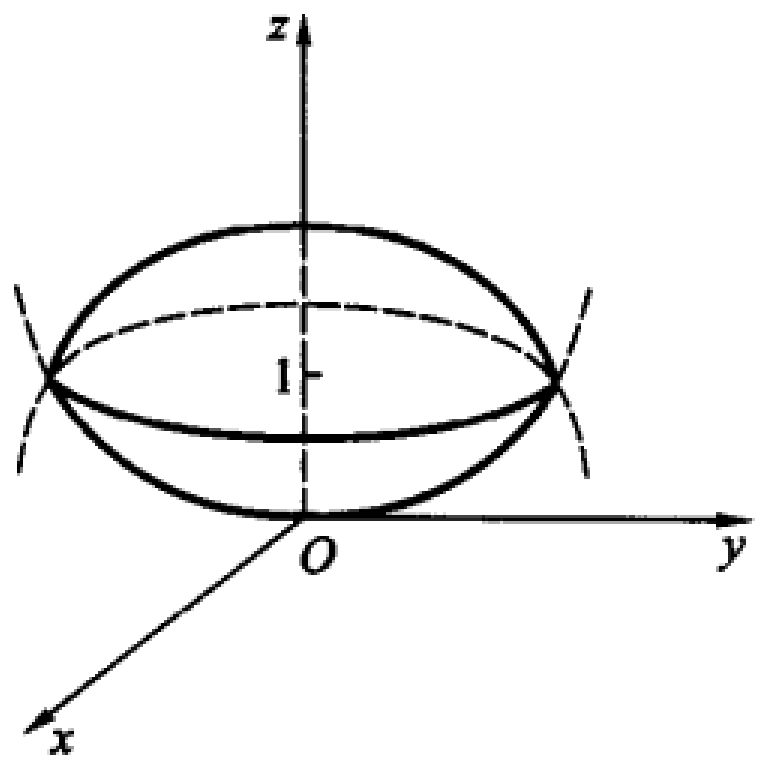
\includegraphics[width=0.28\textwidth]{work/figures/fig20-42}\caption{\relax}\label{fig:20-42}
\end{figure}

两曲面在平面 $z=1$ 上相交，因此
\[
\begin{aligned}
\iiint_{V}z\,\mathrm{d}x\mathrm{d}y\mathrm{d}z&=\int_{0}^{1}z\,\mathrm{d}z\iint_{x^{2}+y^{2}\leqslant z}\mathrm{d}x\mathrm{d}y+\int_{1}^{\sqrt{2}}z\,\mathrm{d}z\iint_{x^{2}+y^{2}\leqslant 2-z^{2}}\mathrm{d}x\mathrm{d}y\\
&=\int_{0}^{1}\pi z^{2}\,\mathrm{d}z+\int_{1}^{\sqrt{2}}\pi z(2-z^{2})\,\mathrm{d}z=\frac{7}{12}\pi.
\end{aligned}
\]
而
\[
\begin{aligned}
\iiint_{V}\mathrm{d}x\mathrm{d}y\mathrm{d}z&=\int_{0}^{1}\mathrm{d}z\iint_{x^{2}+y^{2}\leqslant z}\mathrm{d}x\mathrm{d}y+\int_{1}^{\sqrt{2}}\mathrm{d}z\iint_{x^{2}+y^{2}\leqslant 2-z^{2}}\mathrm{d}x\mathrm{d}y\\
&=\int_{0}^{1}\pi z\,\mathrm{d}z+\int_{1}^{\sqrt{2}}\pi(2-z^{2})\,\mathrm{d}z\\
&=\left(\frac{4}{3}\sqrt{2}-\frac{7}{6}\right)\pi.
\end{aligned}
\]
故
\[
\bar{z}=\frac{\dfrac{7}{12}\pi}{\left(\dfrac{4}{3}\sqrt{2}-\dfrac{7}{6}\right)\pi}=\frac{7}{2(8\sqrt{2}-7)}.
\]
\end{proof}

\subsection{转动惯量}

在第八章中我们曾经利用定积分求过某些特殊类型的平面或空间物体的转动惯量．对于一般的平面或空间物体的转动惯量，则要借助于重积分．

设 $V$ 是空间的一块物体，其密度函数 $\rho(x,y,z)$ 在 $V$ 上连续．我们来求 $V$ 对三坐标轴的转动惯量．对于 $V$ 上的任一体积元素 $\mathrm{d}V$，其质量微元为 $\mathrm{d}m=\rho(x,y,z)\mathrm{d}V$，这时 $\mathrm{d}V$ 对 $x$ 轴，$y$ 轴，$z$ 轴的转动惯量分别为
\[
\begin{aligned}
\mathrm{d}I_{x}&=\left(y^{2}+z^{2}\right)\rho(x,y,z)\mathrm{d}V=\left(y^{2}+z^{2}\right)\mathrm{d}m,\\
\mathrm{d}I_{y}&=\left(x^{2}+z^{2}\right)\rho(x,y,z)\mathrm{d}V=\left(y^{2}+z^{2}\right)\mathrm{d}m,\\
\mathrm{d}I_{z}&=\left(x^{2}+y^{2}\right)\rho(x,y,z)\mathrm{d}V=\left(x^{2}+y^{2}\right)\mathrm{d}m.
\end{aligned}
\]
由于 $V$ 对坐标轴的转动惯量就是所有质量微元对坐标轴的转动惯量的总和，这是三维连续量作用的总和，因此就是对 $\mathrm{d}I_{x}$，$\mathrm{d}I_{y}$，$\mathrm{d}I_{z}$ 求三重积分，故 $V$ 对三坐标轴的转动惯量为
\[
\begin{aligned}
I_{x}&=\iiint_{V}\left(y^{2}+z^{2}\right)\rho(x,y,z)\,\mathrm{d}x\mathrm{d}y\mathrm{d}z,\\
I_{y}&=\iiint_{V}\left(x^{2}+z^{2}\right)\rho(x,y,z)\,\mathrm{d}x\mathrm{d}y\mathrm{d}z,\\
I_{z}&=\iiint\limits_{V}\left(x^{2}+y^{2}\right)\rho(x,y,z)\,\mathrm{d}x\mathrm{d}y\mathrm{d}z.
\end{aligned}
\]
同理可得 $V$ 对坐标面的转动惯量为
\[
\begin{aligned}
I_{xy}&=\iiint_{V}z^{2}\rho(x,y,z)\,\mathrm{d}x\mathrm{d}y\mathrm{d}z,\\
I_{yz}&=\iiint_{V}x^{2}\rho(x,y,z)\,\mathrm{d}x\mathrm{d}y\mathrm{d}z,\\
I_{zx}&=\iiint_{V}y^{2}\rho(x,y,z)\,\mathrm{d}x\mathrm{d}y\mathrm{d}z.
\end{aligned}
\]

平面薄板对轴的转动惯量可类似地讨论．这里仅举例说明．

\begin{example}\label{ex:20-5-2}
求均匀圆盘 $D$：$x^{2}+y^{2}\leqslant R^{2}$ 对于其切线的转动惯量，设密度 $\rho$ 为常数．
\end{example}

\begin{proof}[解]
取切线为 $y=R$．任给面积微元 $\mathrm{d}\sigma$，它对切线 $y=R$ 的转动惯量为 $\mathrm{d}I=(R-y)^{2}\rho\,\mathrm{d}\sigma$．因此 $D$ 对 $y=R$ 的转动惯量为

\begin{figure}[htbp]
\centering
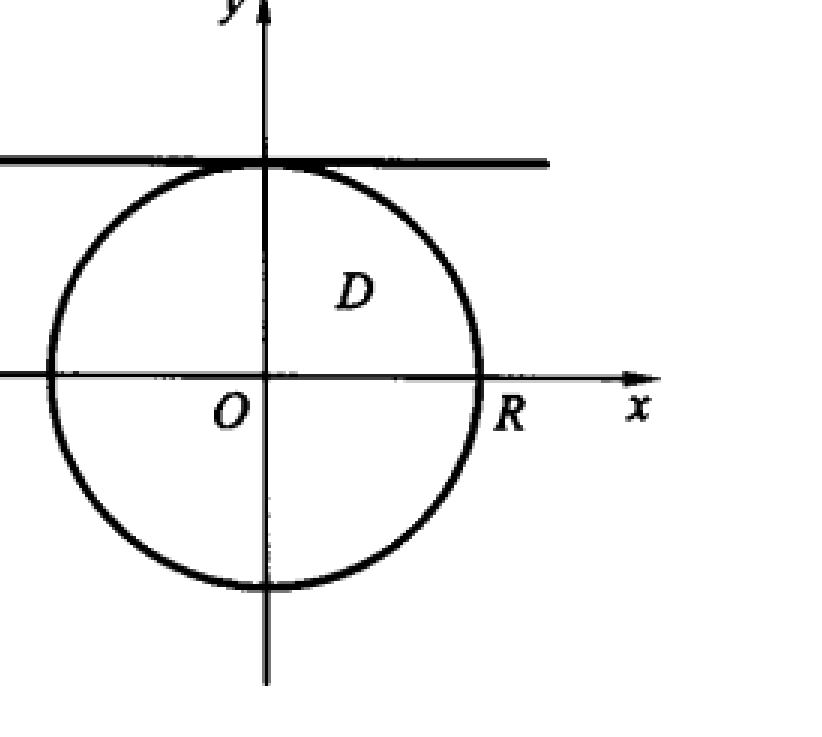
\includegraphics[width=0.28\textwidth]{work/figures/fig20-43}\caption{\relax}\label{fig:20-43}
\end{figure}
\[
\begin{aligned}
I&=\iint\limits_{D}(R-y)^{2}\rho\,\mathrm{d}\sigma\\
&=\rho\int_{0}^{2\pi}\mathrm{d}\theta\int_{0}^{R}(R-r\sin\theta)^{2}r\,\mathrm{d}r\\
&=\rho\int_{0}^{2\pi}\mathrm{d}\theta\int_{0}^{R}\left(R^{2}-2Rr\sin\theta+r^{2}\sin^{2}\theta\right)r\,\mathrm{d}r\\
&=\rho\left(2\pi R^{2}\int_{0}^{R}r\,\mathrm{d}r+\int_{0}^{2\pi}\sin^{2}\theta\,\mathrm{d}\theta\int_{0}^{R}r^{3}\,\mathrm{d}r\right)\\
&=\rho\left(\pi R^{4}+\frac{1}{4}\pi R^{4}\right)=\frac{5}{4}\rho\pi R^{4}.
\end{aligned}
\]
\end{proof}

\begin{example}\label{ex:20-5-3}
设球体的密度与球心的距离成正比，求它对于切平面的转动惯量．
\end{example}

\begin{proof}[解]
设球体的方程为 $x^{2}+y^{2}+z^{2}\leqslant R^{2}$，则密度函数为 $\rho(x,y,z)=k\sqrt{x^{2}+y^{2}+z^{2}}$，其中 $k$ 是比例常数．取切平面方程为 $z=R$，则球体对平面 $z=R$ 的转动惯量为
\[
\begin{aligned}
I&=k\iiint\limits_{V}(R-z)^{2}\sqrt{x^{2}+y^{2}+z^{2}}\,\mathrm{d}x\mathrm{d}y\mathrm{d}z\\
&=k\int_{0}^{2\pi}\mathrm{d}\theta\int_{0}^{R}\mathrm{d}r\int_{0}^{\pi}(R-r\cos\varphi)^{2}r^{3}\sin\varphi\,\mathrm{d}\varphi\\
&=2\pi k\int_{0}^{R}r^{2}\left.\frac{1}{3}(R-r\cos\varphi)^{3}\right|_{0}^{\pi}\,\mathrm{d}r\\
&=\frac{2}{3}\pi k\int_{0}^{R}r^{2}\left[(R+r)^{3}-(R-r)^{3}\right]\mathrm{d}r\\
&=\frac{4}{3}\pi k\int_{0}^{R}r^{2}\left(3R^{2}r+r^{3}\right)\mathrm{d}r=\frac{11}{9}\pi kR^{6}.
\end{aligned}
\]
\end{proof}

\begin{figure}[htbp]
\centering
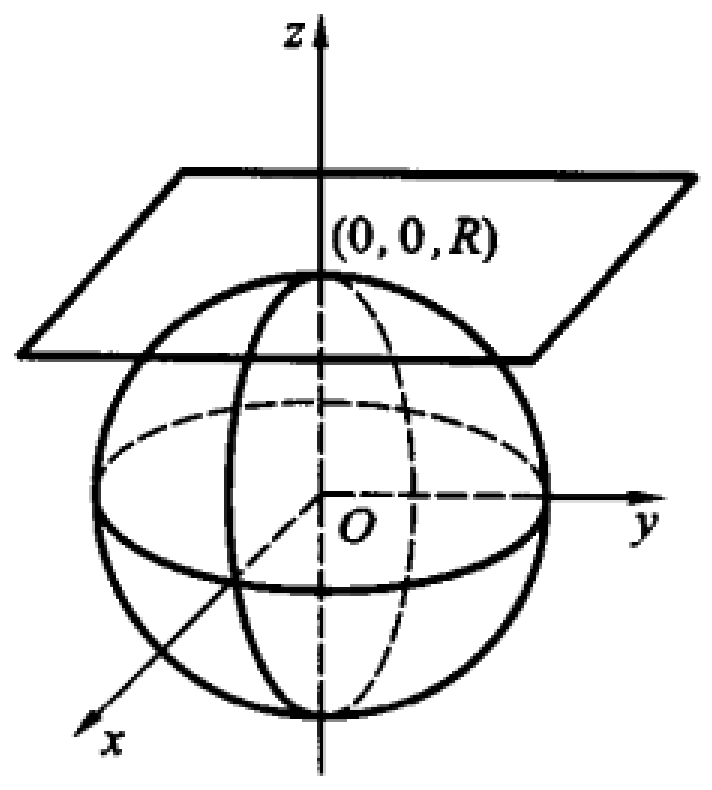
\includegraphics[width=0.26\textwidth]{work/figures/fig20-44}\caption{\relax}\label{fig:20-44}
\end{figure}

\subsection{引力}

设 $V$ 是空间的一块物体，密度函数 $\rho(x,y,z)$ 在 $V$ 上连续．求 $V$ 对 $V$ 外一点 $(x_{0},y_{0},z_{0})$ 处质量为 $1$ 的质点 $A$ 的引力 $\bm{F}$．任取 $V$ 上的质量微元 $\mathrm{d}m=\rho(x,y,z)\mathrm{d}V$．$A$ 到 $\mathrm{d}m$ 的向量为 $\bm{r}=(x-x_{0},y-y_{0},z-z_{0})$．这时 $\mathrm{d}m$ 对 $A$ 的引力为
\[
\mathrm{d}\bm{F}=\frac{k\rho(x,y,z)}{r^{3}}(x-x_{0},y-y_{0},z-z_{0})\,\mathrm{d}V,
\]
其中 $k$ 是引力常数，$r=\sqrt{(x-x_{0})^{2}+(y-y_{0})^{2}+(z-z_{0})^{2}}$．对 $V$ 求和，便得 $\bm{F}$ 在三坐标轴上的投影分别为
\[
\begin{aligned}
F_{x}&=\iiint\limits_{V}k\frac{x-x_{0}}{r^{3}}\rho(x,y,z)\,\mathrm{d}x\mathrm{d}y\mathrm{d}z,\\
F_{y}&=\iiint\limits_{V}k\frac{y-y_{0}}{r^{3}}\rho(x,y,z)\,\mathrm{d}x\mathrm{d}y\mathrm{d}z,\\
F_{z}&=\iiint\limits_{V}k\frac{z-z_{0}}{r^{3}}\rho(x,y,z)\,\mathrm{d}x\mathrm{d}y\mathrm{d}z.
\end{aligned}
\]
而 $\bm{F}=F_{x}\,\bm{i}+F_{y}\,\bm{j}+F_{z}\,\bm{k}$．

\begin{figure}[htbp]
\centering
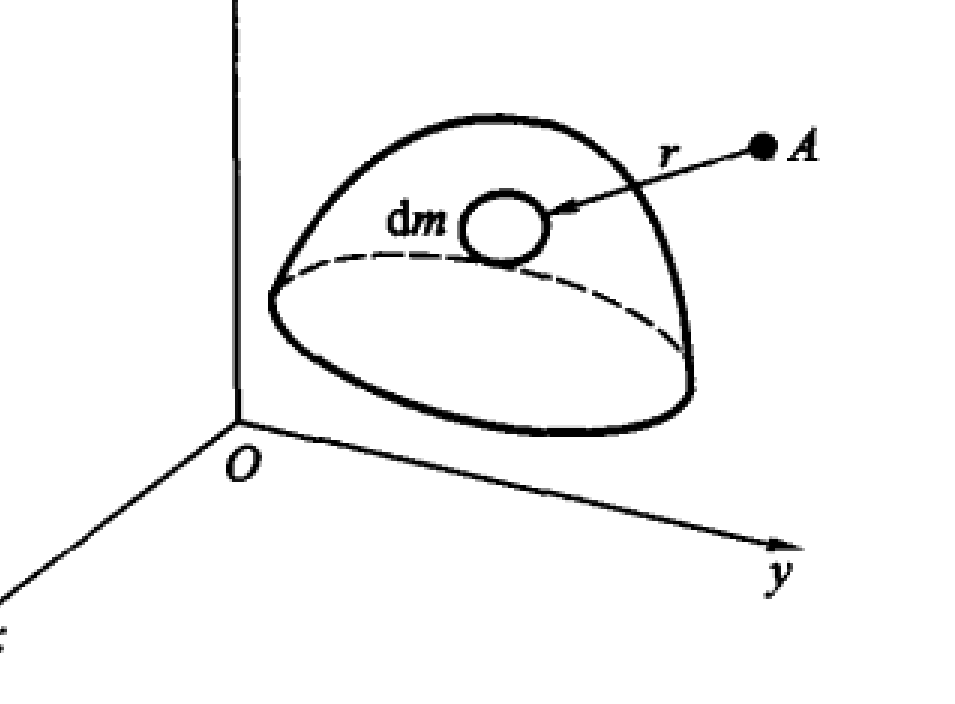
\includegraphics[width=0.32\textwidth]{work/figures/fig20-45}\caption{\relax}\label{fig:20-45}
\end{figure}

\begin{example}\label{ex:20-5-4}
求均匀球体 $x^{2}+y^{2}+z^{2}\leqslant R^{2}$ 对球外一点质量为 $1$ 的质点 $A$ 的引力．
\end{example}

\begin{proof}[解]
设球体的密度为常数 $\rho$，不妨设质点 $A$ 位于 $z$ 轴 $(0,0,h)$ 处 $(h>R)$．由对称性知 $F_{x}=F_{y}=0$．
\[
F_{z}=k\rho\iiint_{V}\frac{z-h}{\left[x^{2}+y^{2}+(z-h)^{2}\right]^{\frac{3}{2}}}\,\mathrm{d}x\mathrm{d}y\mathrm{d}z.
\]
作柱坐标变换，得
\[
\begin{aligned}
F_{z}&=k\rho\int_{0}^{2\pi}\mathrm{d}\theta\int_{-R}^{R}(z-h)\,\mathrm{d}z\int_{0}^{\sqrt{R^{2}-z^{2}}}\frac{r\,\mathrm{d}r}{\left[r^{2}+(z-h)^{2}\right]^{\frac{3}{2}}}\\
&=2\pi k\rho\int_{-R}^{R}\left(-1-\frac{z-h}{\sqrt{R^{2}+h^{2}-2hz}}\right)\mathrm{d}z\\
&=-\frac{4}{3h^{2}}\pi k\rho R^{3}.
\end{aligned}
\]
这个结果表明球体对质点 $A$ 的引力等于将球体的全部质量 $\dfrac{4}{3}\pi R^{3}\rho$ 集中于球心时对质点 $A$ 的引力．
\end{proof}

\begin{xiti}
\item 求下列均匀密度的平面薄板的质心：
\begin{ziti}
\item 半椭圆 $\dfrac{x^{2}}{a^{2}}+\dfrac{y^{2}}{b^{2}}\leqslant 1$，$\quad y\geqslant 0$；
\item 高为 $h$，底分别为 $a$ 和 $b$ 的等腰梯形；
\item $r=a(1+\cos\varphi)$ $(0\leqslant\varphi\leqslant\pi)$ 所界的薄板；
\item $ay=x^{2}$，$x+y=2a$ $(a>0)$ 所界的薄板．
\end{ziti}
\item 求下列密度均匀的物体的质心：
\begin{ziti}
\item $z\leqslant 1-x^{2}-y^{2}$，$z\geqslant 0$；
\item 由坐标面及平面 $x+2y-z=1$ 所围的四面体；
\item $z=x^{2}+y^{2}$，$x+y=a$，$x=0$，$y=0$，$z=0$ 围成的立体；
\item $z^{2}=x^{2}+y^{2}$ $(z\geqslant 0)$ 和平面 $z=h$ 围成的立体；
\item 半球壳 $a^{2}\leqslant x^{2}+y^{2}+z^{2}\leqslant b^{2}$，$\quad z\geqslant 0$．
\end{ziti}
\item 求下列密度均匀的平面薄板的转动惯量：
\begin{ziti}
\item 边长为 $a$ 和 $b$，且夹角为 $\varphi$ 的平行四边形，关于底边 $b$ 的转动惯量；
\item $y=x^{2}$，$y=1$ 所围平面图形关于直线 $y=-1$ 的转动惯量．
\end{ziti}
\item 求由下列曲面所界均匀体的转动惯量：
\begin{ziti}
\item $z=x^{2}+y^{2}$，$x+y=\pm 1$，$x-y=\pm 1$，$z=0$ 关于 $z$ 轴的转动惯量；
\item 长方体关于它的一棱的转动惯量；
\item 圆筒 $a^{2}\leqslant x^{2}+y^{2}\leqslant b^{2}$，$-h\leqslant z\leqslant h$ 关于 $x$ 轴和 $z$ 轴的转动惯量．
\end{ziti}
\item 设球体 $x^{2}+y^{2}+z^{2}\leqslant 2x$ 上各点的密度等于该点到坐标原点的距离，求这球的质量．
\item 求均匀薄片 $x^{2}+y^{2}\leqslant R^{2}$，$z=0$ 对 $z$ 轴上一点 $(0,0,c)$ $(c>0)$ 处单位质点的引力．
\item 求均匀柱体 $x^{2}+y^{2}\leqslant a^{2}$，$0\leqslant z\leqslant h$ 对于 $(0,0,c)$ $(c>h)$ 处单位质点的引力．
\end{xiti}


